\documentclass[
    ngerman,
    color=3b,
    % dark_mode, 
    load_common, % Loads a list of commonly used Packages
    summary,
    boxarc,
    % manual_term,
    % solution=true,
]{tuda_summary}
 
\externaldocument{../Kapitel_1/Kapitel_1}
\externaldocument{../Kapitel_2/Kapitel_2}
\externaldocument{../Kapitel_3/Kapitel_3}
\externaldocument{../Kapitel_4/Kapitel_4}
\externaldocument{../Kapitel_5/Kapitel_5}
\externaldocument{../Kapitel_6/Kapitel_6}
\externaldocument{../Kapitel_7/Kapitel_7}
\externaldocument{../Kapitel_8/Kapitel_8}
 
\title[AuD]{Algorithmen\\und Datenstrukturen}
\subtitle{Zusammenfassung}
% \subsubtitle{test}
\semester{SoSe 2020}
\fachbereich{Informatik}
\author{Ruben Deisenroth}
\contributor{J. Milkovits}
\date{\today}
\version{2.0.1 (SNAPSHOT)}
\termOrder{printAuthor,printSemester,printContributor,%
printVersion,,,printDate,printFachbereich}

\ConfigureHeadline{
	headline={summary-centered}
}

%\def\isMain{true}
\begin{document}

%--Titelseite--
\maketitle{}
\tableofcontents %Inhaltsverzeichnis
\clearpage
%---Beginn Der Zusammenfassung---%

%Kapitel Laden
% Dieser Ansatz lässt keine preview von LaTeX-Workshop zu
%\foreach \kapitelnr in {1,...,8}{
%    \input{Kapitel/Kapitel_\kapitelnr/Kapitel_\kapitelnr}
%}
%Dieser schon
\documentclass[
    ngerman,
    color=3b,
    % dark_mode,
    load_common, % Loads a list of commonly used Packages
    summary,
    boxarc,
    % manual_term,
    % solution=true,
]{rubos-tuda-template} 
% Import all Packages from Main Preamble with relative Path
% \subimport*{../../}{preamble}
% Get Labels from Main Document using the xr-hyper Package
\externaldocument{../../AuD-Zusammenfassung-2020}
% Set Graphics Path, so pictures load correctly
\graphicspath{{../../}}

\begin{document}
\section{Einführung}\label{1}\label{Einfuehrung}
\subsection{Probleme in der Informatik}\label{1.1}
Ein \fatsf{Problem}\index{Problem} im Sinne der Informatik:
\begin{itemize}
    \item Enthält Beschreibung der Eingabe
    \item Enthält Beschreibung der Ausgabe
    \item Gibt selbst \fatsf{keinen} Übergang von Ein und Ausgabe an
\end{itemize}
\begin{figure}[ht]
    \centering
    \includestandalone[width=.5\textwidth]{pictures/problem_informatik_modell/problem_informatik_modell}% 
    \caption{Modell Problem Informatik}
    \label{fig:modell-problem-informatik}
\end{figure}
z.B. Finde den kürzesten Weg zwischen 2 Orten\\
Eine \fatsf{Probleminstanz}\index{Probleminstanz} ist eine konkrete Eingabebelegung für die entsprechende Ausgabe gewünscht.\\
Für das obige Problem wäre das z.B. "`Was ist der kürzeste Weg vom Audimax in die Mensa?"'
\subsection{Definitionen für Algorithmen}\label{1.2}\label{Definitionen fuer Algorithmen}\index{Algorithmen}
\begin{definition}[Algorithmus]
    \enquote{Ein Algorithmus ist eine \fatsf{endliche Folge} von Rechenschritten, die eine \fatsf{Eingabe} in eine \fatsf{Ausgabe} umwandelt.}\footnote{Quelle: Cormen et al., 4. Auflage}
\end{definition}
\paragraph{Anforderungen an Algorithmen:}
\begin{description}[leftmargin=7cm, itemsep=1em]
    \item[Spezifizierung der Ein- und Ausgabe] \begin{itemize}
        \item Anzahl und Typen aller Elemente ist/sind definiert
    \end{itemize}
    \item[Eindeutigkeit]\index{Eindeutigkeit}\begin{itemize}
        \item Jeder Einzelschritt ist klar definiert und ausführbar
        \item Die Reihenfolge der Einzelschritte ist festgelegt.
    \end{itemize}
    \item[Endlichkeit]\index{Endlichkeit}\begin{itemize}
        \item Notation hat endliche Länge
    \end{itemize}
\end{description}
\paragraph{Eigenschaften von Algorithmen:}
\begin{description}[leftmargin=3.5cm]
    \item[Determiniertheit]\index{Determiniertheit} Für gleiche Eingabe folgt stets die gleiche Ausgabe (andere Zwischenzustände sind möglich)
    \item[Determinismus]\index{Determinismus} Für die gleiche Eingabe ist die Ausführung und Ausgabe stets identisch.
    \item[Terminierung]\index{Terminierung} Der Algorithmus läuft für jede endliche Eingabe nur endlich lange
    \item[Korrektheit]\index{Korrektheit} Der Algorithmus berechnet stets die spezifizierte Ausgabe (falls dieser terminiert).
    \item[Effizienz]\index{Effizienz} Sparsamkeit im Ressourcenverbrauch (Zeit, Speicher, Energie, ...)
\end{description}
\subsection{Definitionen für Datenstrukturen}\label{1.3}\label{Definitionen fuer Datenstrukturen}\index{Datenstrukturen}
\begin{definition}[Datenstruktur]
    \enquote{Eine Datenstruktur ist eine Methode,
    Daten \fatsf{abzuspeichern} und zu \fatsf{organisieren} sowie
    den \fatsf{Zugriff} auf die Daten und die \fatsf{Modifikation}
    der Daten zu erleichtern.}\footnote{Quelle: Cormen et al., 4. Auflage}\\
\end{definition}
\begin{wrapfigure}[5]{r}{.6\textwidth}
    \centering
    \includestandalone[width=.5\textwidth]{pictures/baum_beispiel/baum_beispiel}% 
    \caption{Beispiel Datenstruktur (Rot-Schwarz-Baum)}
    \label{fig:baum_beispiel}
\end{wrapfigure}
Datenstrukturen:\begin{itemize}
    \item Sind Organisationsformen für Daten
    \item Beinhalten Strukturbestandteile und Nutzerdaten (Payload)
\end{itemize}
z.B. \hyperref[2.2]{Arrays}, Listen, \ldots
\vspace*{2cm}
\subsection{Pseudocode-Konventionen}\index{Pseudocode}
\begin{grayInfoBox}
    \begin{itemize}
        \item Blöcke werden durch Einrückungen hervorgehoben
        \item Blockkonstrukte sind "`\texttt{for x to y}"', "`\texttt{while}"', "`\texttt{repeat-until}"' und "`\texttt{if-else}"'
        \item Kommentare erhalten das Prädikat "`\texttt{//}"'
        \item "`\texttt{i = j = e}"' bedeutet, \texttt{i} und \texttt{j} erhalten den Wert von \texttt{e}
        \item Variablen sind immer lokal
        \item $A[i]$ bezeichnet das i-te Element im Array A
        \item $A[i..j]$ Array A im Bereich von $i-j$
        \item Attribute werden über einen "`\texttt{.}"' abgerufen
    \end{itemize}
\end{grayInfoBox}

\subsection{Weitere wichtige Definitionen}
\begin{definition}[short circuit evaluation (Kurzschlussauswertung)]\index{short circuit evaluation}
    Strategie, bei der die Auswertung, nachdem die \linebreak Gesamtlösung durch einen Teilausdruck eindeutig bestimmt wurde, abgebrochen wird.\\ 
    z.B.: \texttt{1+1==2 || 1/0==0}$\longrightarrow \texttt{true}$
\end{definition}
\begin{definition}[call-by-reference (Referenzparameter)]\index{call-by-reference}
    Übergeben von Referenz auf ein Objekt. Dadurch sind Änderungen an diesem innerhalb der Routine möglich.
\end{definition}
\begin{definition}[call-by-value (Wertparameter)]index{call-by-value}
    Übergeben einer Kopie des Objekts. Das ursprüngliche Objekt kann so nicht mehr verändert werden, jedoch die Kopie. Die referenzen bleiben beim Kopieren gleich\linebreak (z.B. bein Linked List)
\end{definition}
\clearpage
\end{document}
\documentclass[
    12pt,
    a4paper,
    ngerman,
    color=3b,% Farbe für Hervorhebungen auf Basis der Deklarationen in den
    %type=intern,
    %titlepage=true,
    marginpar=false,
    colorback=false,
    %logo=head,
    leqno,
]{tudaexercise}
\usepackage{import}
% Import all Packages from Main Preamble with relative Path
\subimport*{../../}{preamble}
% Get Labels from Main Document using the xr-hyper Package
\externaldocument{../../AuD-Zusammenfassung-2020}
% Set Graphics Path, so pictures load correctly
\graphicspath{{../../}}

\begin{document}

\section{Sortieren}\label{2}\label{Sortieren}\index{Sortieren}
\subsection{Einführung}\label{2.1}\label{Einfuehrung Sortieren}
Das Sortierproblem\index{Sortierproblem}\\
\begin{itemize}
    \item Ausgangspunkt: Folge von Datensätzen $D_1,D_2,\cdots,D_n$
          \begin{figure}[h]
              \centering
              \includestandalone[width=.2\textwidth]{pictures/folge_von_Datensätzen/folge_von_Datensätzen}% 
              %\caption{Beispiel Datenstruktur (Rot-Schwarz-Baum)}
              \label{fig:folge_von_Datensätzen}
          \end{figure}
          \vspace*{-1em}
    \item zu sortierende Elemente heißen auch Schlüssel(werte)
    \item Ziel:  Datensätze so anzuordnen, dass die Schlüsselwerte sukzessive
          ansteigen (oder absteigen)
    \item Bedingung: Schlüssel(werte) müssen vergleichbar sein
\end{itemize}
Durchführung:\begin{itemize}
    \item Eingabe: Sequenz von Schlüsselwerten $\left\{a_1,a_2,\ldots,a_n\right\}$
    \item Eingabe ist eine \fatsf{Instanz} des Sortierproblems
    \item Ausgabe: Permutation $\left\{a_1',a_2',\ldots,a_n'\right\}$ derselben Folge mit Eigenschaft $a_1'\leq\ldots\leq a_n'$
    \item Algorithmus \fatsf{korrekt}, wenn dieser das Problem für alle Instanzen löst
\end{itemize}
\clearpage
\subsection{Arrays}\label{2.2}\label{Arrays}\index{Array}
Reihung (Feld) fester Länge von Daten des gleichen Typs
\begin{figure}[h]
    \centering
    \includestandalone[]{pictures/array_beispiel/array_beispiel}% 
    \caption{beispielhafte Darstellung eines Arrays}
    \label{fig:folge_von_Datensätzen}
\end{figure}
\begin{itemize}
    \item $A$: Bezeichnung des Arrays mit dem Namen "`$A$"'
    \item $A[i]$: Zugiff auf das $(i+1)$-te Element des Arrays
\end{itemize}
Beispiel: $A[2]=17$\\
$\Longrightarrow$ Arrays erlauben effizienten Zugriff auf Elemente: konstanter Aufwand
\subsection{Exkurs: Totale Ordnung}\label{Totale Ordnung}\index{Totale Ordnung}
Sei $M$ eine nicht leere Menge und $\leq \subseteq M\times M $ eine binäre Relation auf $M$.

Das Paar $(M,\leq)$ heißt genau dann eine totale Relation auf der Menge $M$, wenn folgende Eigenschaften erfüllt sind:
\begin{itemize}
    \item Reflexivität: $\forall x \in M: x \leq x$
    \item Transitivität: $\forall x,y,z\in M: x\leq y \land y \leq z \Rightarrow x \leq z$
    \item Antisymmetrie: $\forall x,y\in M: x\leq y \land y \leq x \Rightarrow x = y$
    \item Totalität: $\forall x,y \in M : x\leq y \lor y \leq x$
\end{itemize}
Beispiele:\begin{itemize}
    \item $\leq$ Ordnung auf natürlichen Zahlen
    \item Lexikographische Ordnung $\leq_{lex}$ ist eine totale Ordnung
\end{itemize}
\subsection{Vergleichskriterien von Suchalgorithmen}\label{Vergleichskriterien von Suchalgorithmen}
\begin{itemize}
    \item Berechnungsaufwand: $\mathcal{O}(n)$
    \item Effizienz: Best Case vs. Average Case vs Worst Case
    \item Speicherbedarf:\begin{itemize}
              \item in-Place (in situ): zusätzlicher Speicher von der Eingabegröße unabhängig
              \item out-of-place: Speichermehrbedarf von Eingabegröße abhängig
          \end{itemize}
    \item Stabilität: stabile Verfahren verändern die Reihenfolge von äquivalenten Elementen nicht
    \item Anwendung als Auswahlfaktor:\begin{itemize}
              \item Hauptoperationen beim Sortieren: Vergleichen und Vertauschen
              \item Anwendung spielt eine enorme Rolle:\begin{itemize}
                        \item Verfahren mit vielen Vertauschungen und wenig Vergleichen, wenn Vergleichen teuer
                        \item Verfahren mit wenig Vertauschungen und vielen Vergleichen, wenn Umsortieren teuer
                    \end{itemize}
          \end{itemize}
\end{itemize}
\subsection{Analyse von Algorithmen \textmd{(I)}}\label{Analyse von Algorithmen 1}
\begin{itemize}

    \item \fatsf{Schleifeninvariante \textmd{(SIV)}:}\index{Schleifeninvariante}
          \begin{itemize}
              \item Sonderform der Invariante
              \item Am Anfang/Ende jedes Schleifendurchlaufs und vor/nach jedem Schleifendurchlauf gültig
              \item Wird zur Feststellung der Korrektheit von Algorithmen verwendet
              \item Eigenschaften:
                    \begin{itemize}
                        \item Initialisierung: Invariante ist vor jeder Iteration wahr
                        \item Fortsetzung: Wenn SIV vor der Schleife wahr ist, dann auch bis Beginn der nächsten Iteration
                        \item Terminierung: SIV liefert bei Schleifenabbruch, helfende Eigenschaft für Korrektheit
                    \end{itemize}
              \item Beispiel für Umsetzung: \hyperref[insSortSiv]{\textcolor{red}{Insertion Sort - SIV}}
          \end{itemize}

    \item \fatsf{Laufzeitanalyse:}\index{Laufzeitanalyse}
          \begin{itemize}
              \item Aufstellung der Kosten und Durchführungsanzahl für jede Zeile des Quelltextes
              \item Beachte: Bei Schleifen wird auch der Aufruf gezählt, der den Abbruch einleitet
              \item Beispiel für Umsetzung: \hyperref[insSortLaufzeit]{\textcolor{red}{Insertion Sort - Laufzeit}}
              \item Zusätzliche Überprüfung des \texttt{Best Case, Worst Case} und \texttt{Average Case}
          \end{itemize}

    \item \fatsf{Effizienz von Algorithmen}\index{Effizienz von Algorithmen}:
          \begin{itemize}
              \item Effizienzfaktoren
                    \begin{itemize}
                        \item Rechenzeit (Anzahl der Einzelschritte)
                        \item Kommunikationsaufwand
                        \item Speicherplatzbedarf
                        \item Zugriffe auf Speicher
                    \end{itemize}
              \item Laufzeit hängt von versch. Faktoren ab
                    \begin{itemize}
                        \item Länge der Eingabe
                        \item Implementierung der Basisoperationen
                        \item Takt der CPU
                    \end{itemize}
          \end{itemize}

\end{itemize}
\clearpage
\subsection{Analyse von Algorithmen \textmd{(II)}}\label{Analyse von Algorithmen 2}
\begin{itemize}
    \item \fatsf{Komplexität:}
          \begin{itemize}
              \item Abstrakte Rechenzeit $T(n)$ ist abhängig von den Eingabedaten
              \item Übliche Betrachtungsweise der Rechenzeit ist asymptotische Betrachtung
          \end{itemize}

    \item \fatsf{Asymptotik:}
          \begin{itemize}
              \item Annäherung an einer sich ins Unendliche verlaufende Kurve
              \item z.B.: $f(x) = \frac{1}{x} + x$ | Asymptote: $g(x)=x$ | ($\frac{1}{x}$ läuft gegen Null)
          \end{itemize}

    \item \fatsf{Asymptotische Komplexität:}
          \begin{itemize}
              \item Abschätzung des zeitlichen Aufwands eines Algorithmus in Abhängigkeit einer Eingabe
              \item Beispiel für Umsetzung: \hyperref[insSortLaufzeitTheta]{\textcolor{red}{Insertion Sort - Laufzeit $\Theta$}}
          \end{itemize}

    \item \fatsf{Asymptotische Notation:}
          \begin{itemize}
              \item Betrachtung der Laufzeit $T(n)$ für sehr gro\ss e Eingaben $n \in \mathbb{N}$
              \item Komplexität ist unabhängig von konstanten Faktoren und Summanden
              \item Nicht berücksichtigt: Rechnergeschwindigkeit / Initialisierungsaufwände
              \item Komplexitätsmessung via Funktionsklasse ausreichend
                    \begin{itemize}
                        \item Verhalten des Algorithmus für gro\ss e Problemgrö\ss en
                        \item Veränderung der Laufzeit bei Verdopplung der Problemgrö\ss e
                    \end{itemize}
          \end{itemize}

    \item \textbf{Gründe für die Nutzung der theoretischen Betrachtung statt der Messung der Laufzeit }
          \begin{itemize}
              \item \textit{Vergleichbarkeit}
                    \begin{itemize}
                        \item Laufzeit abhängig von konkreter Implementierung und System
                        \item Theoretische Betrachung ist frei von Abhängigkeiten und Seiteneffekten
                        \item Theoretische Betrachtung lässt direkte Vergleichbarkeit zu
                    \end{itemize}

              \item \textit{Aufwand}
                    \begin{itemize}
                        \item Wieviele Testreihen?
                        \item In welcher Umgebung?
                        \item Messen führt in der Ausführung zu hohem, praktischen Aufwand
                    \end{itemize}

              \item \textit{Komplexitätsfunktion}
                    \begin{itemize}
                        \item Wachstumsverhalten ausreichend
                        \item Praktische Evaluation mit Zeiten nur für Auswahl von Systemen möglich
                        \item Theoretischer Vergleich (Funktionsklassen) hat ähnlichen Erkenntnisgewinn
                    \end{itemize}
          \end{itemize}
\end{itemize}
\clearpage
\subsection{Analyse von Algorithmen \textmd{(III)}}\label{Analyse von Algorithmen 3}
\begin{itemize}
    \item \textbf{$\Theta$-Notation}
          \begin{itemize}
              \item $\Theta$-Notation beschränkt eine Funktion asymptotisch von oben und unten
              \item Funktionen $f,g: \mathbb{N} \rightarrow \mathbb{R}_{>0}$ ($\mathbb{N}$: Eingabelänge, $\mathbb{R}$: Zeit)
              \item[] 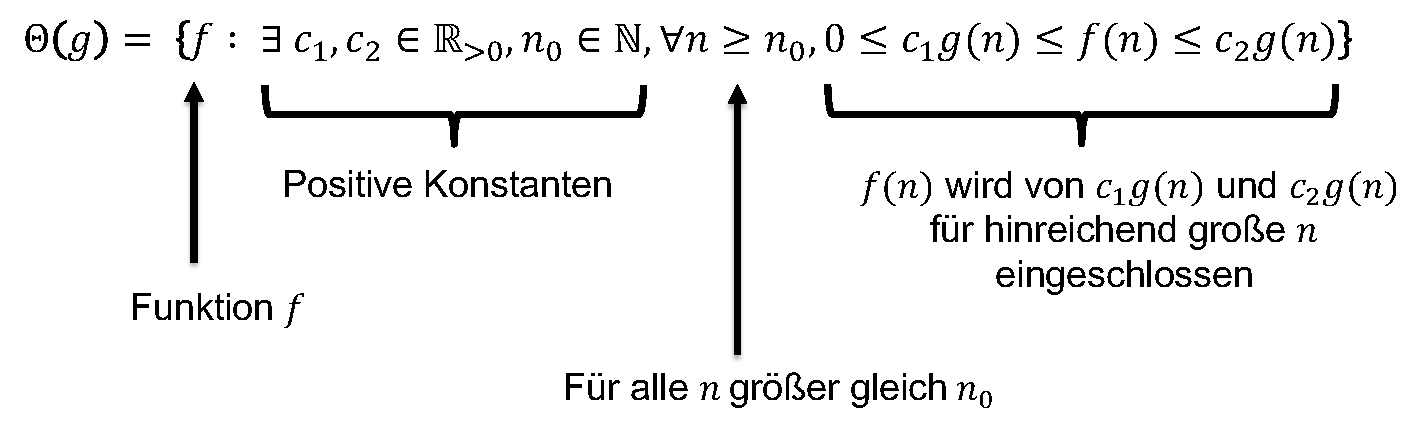
\includegraphics[width=12cm]{pictures/thetaNotation.pdf}
              \item $\Theta(g)$ enthält alle $f$, die genauso schnell wachsen wie $g$
              \item Schreibweise: $f \in \Theta(g)$ (korrekt), manchmal auch $f = \Theta(g)$
              \item $g(n)$ ist eine asymptotisch scharfe Schranke von $f(n)$
              \item $f(n)= \Theta(g(n))$ gilt, wenn $f(n) = O(g(n))$ und $f(n)=\Omega(g(n))$ erfüllt sind
              \item[]
              \item[]
                    \begin{minipage}{0.3\textwidth}
                        \begin{figure}[H]
                            \centering
                            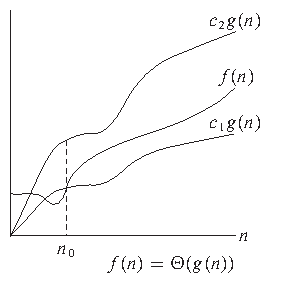
\includegraphics[width=5cm]{pictures/thetaNotationGraph.pdf}
                            \caption{Veranschaulichung}
                            \label{}
                        \end{figure}
                    \end{minipage}
                    \begin{minipage}[t]{0.6\textwidth}
                        \vspace{-3cm}
                        \begin{itemize}
                            \item z.B.: $f(n)= \frac{1}{2} n^2 - 3n$ | $f(n) \in \Theta(n^2)$?
                            \item Aus $\Theta(n^2)$ folgt, dass $g(n)=n^2$
                            \item Vorgehen:
                                  \begin{itemize}
                                      \item Finden eines $n_0$ und $c_1,c_2$, sodass
                                      \item $c_1*g(n) \leq f(n) \leq c_2*g(n)$ erfüllt ist
                                      \item Konkret: $c_1*n^2 \leq \frac{1}{2} n^2 - 3n \leq c_2*n^2$
                                      \item Division durch $n^2$: $c_1 \leq \frac{1}{2}-\frac{3}{n} \leq c2$
                                      \item Ab $n=7$ positives Ergebnis: $0,0714$ | $n_0 = 7$
                                      \item Deswegen setzen wir $c_1=\frac{1}{14}$
                                      \item Für $n \rightarrow \infty: ~ 0,5$ | $c_2 = 0,5$
                                      \item Natürlich auch andere Konstanten möglich
                                  \end{itemize}
                        \end{itemize}
                    \end{minipage}
          \end{itemize}

          \pagebreak

    \item \textbf{$O$-Notation}
          \begin{itemize}
              \item $O$-Notation beschränkt eine Funktion asymptotisch von oben
              \item[] 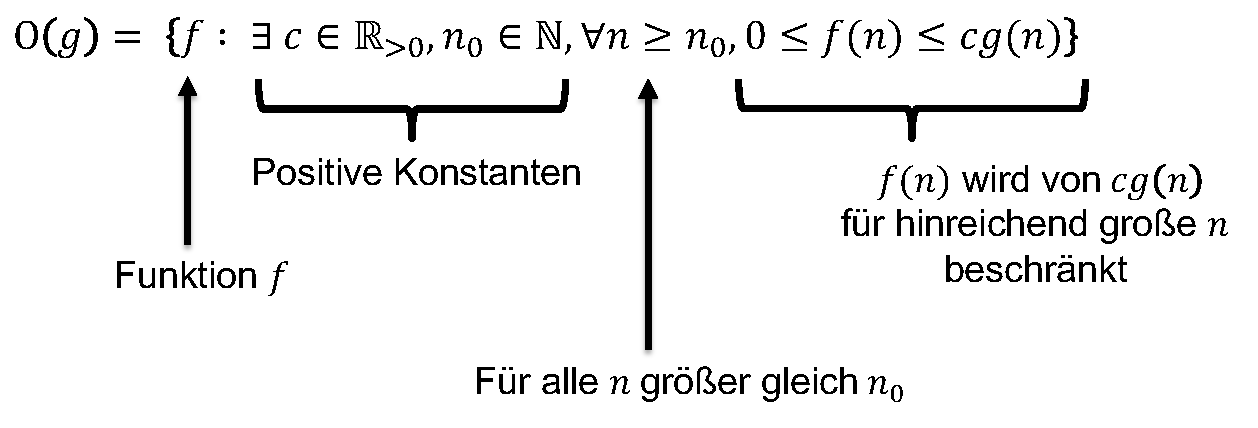
\includegraphics[width=12cm]{pictures/oNotation.pdf}
              \item $O(g)$ enthält alle $f$, die höchstens so schnell wie $g$ wachsen
              \item Schreibweise: $f=O(g)$
              \item $f(n)=\Theta(g) \rightarrow f(n) = O(g)$ | $\Theta(g(n)) \subseteq O(g(n))$
              \item Ist $f$ in der Menge $\Theta(g)$, dann auch in der Menge $O(g)$
              \item[]
              \item[]
                    \begin{minipage}{0.3\textwidth}
                        \begin{figure}[H]
                            \centering
                            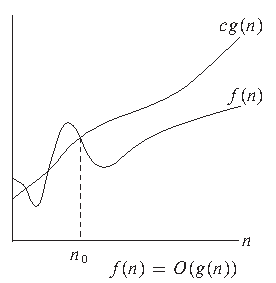
\includegraphics[width=5cm]{pictures/oNotationGraph.pdf}
                            \caption{Veranschaulichung}
                            \label{}
                        \end{figure}
                    \end{minipage}
                    \begin{minipage}[t]{0.6\textwidth}
                        \vspace{-3cm}
                        \begin{itemize}
                            \item z.B.: $f(n) = n + 2$ | $f(n) = O(n)$?
                            \item Ja $f(n)$ ist Teil von $O(n)$ für z.B. $c = 2$ und $n_0 = 2$
                        \end{itemize}
                    \end{minipage}
          \end{itemize}

    \item \textbf{$O$-Notation Rechenregeln}
          \begin{itemize}
              \item Konstanten:
                    \begin{itemize}
                        \item $f(n) = a$ mit $a \in \mathbb{R}$ konstante Funktion $\rightarrow$ $f(n) = O(1)$
                        \item z.B. $3 \in O(1)$
                    \end{itemize}

              \item Skalare Multiplikation:
                    \begin{itemize}
                        \item $f= O(g)$ und $a \in \mathbb{R}$ $\rightarrow$ $a*f = O(g)$
                    \end{itemize}

              \item Addition:
                    \begin{itemize}
                        \item $f_1 = O(g_1)$ und $f_2 = O(g_2)$ $\rightarrow$ $f_1+f_2= O(max\{g_1,g_2\})$
                    \end{itemize}

              \item Multiplikation:
                    \begin{itemize}
                        \item $f_1 = O(g_1)$ und $f_1 = O(g_2)$ $\rightarrow$ $f_1*f_2= O(g_1*g_2)$
                    \end{itemize}
          \end{itemize}

          \pagebreak

    \item \textbf{$\Omega$-Notation}
          \begin{itemize}
              \item $\Omega$-Notation beschränkt eine Funktion asymptotisch von unten
              \item[] 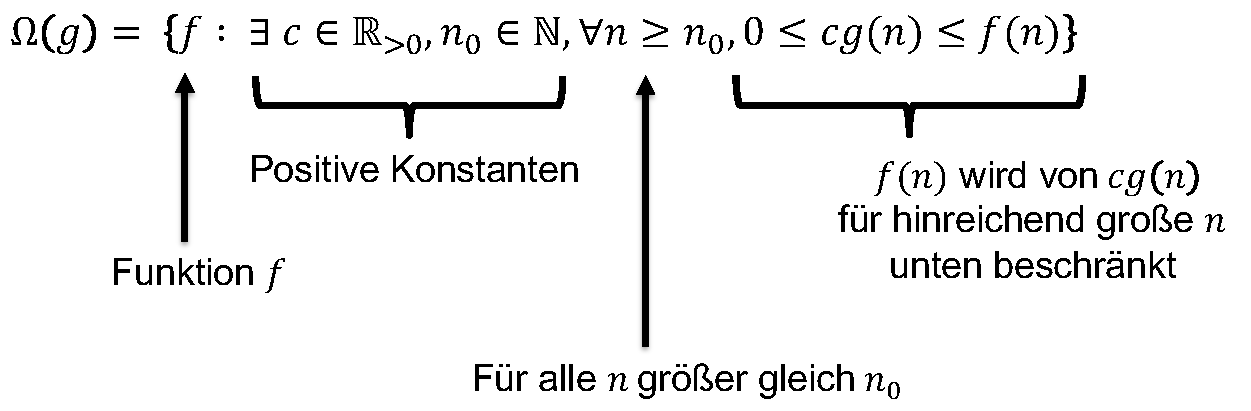
\includegraphics[width=12cm]{pictures/omegaNotation.pdf}
              \item $\Omega$-Notation enthält alle $f$, die mindestens so schnell wie $g$ wachsen
              \item Schreibweise: $f = \Omega(g)$
              \item[]
              \item[]
                    \begin{minipage}{0.3\textwidth}
                        \begin{figure}[H]
                            \centering
                            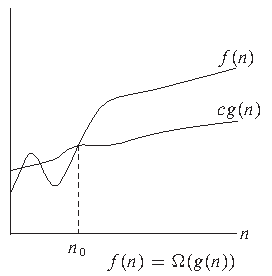
\includegraphics[width=5cm]{pictures/omegaNotationGraph.pdf}
                            \caption{Veranschaulichung}
                            \label{}
                        \end{figure}
                    \end{minipage}
                    \begin{minipage}[t]{0.6\textwidth}
                        \vspace{-3cm}
                    \end{minipage}
          \end{itemize}
          \clearpage
    \item \textbf{Komplexitätsklassen}
          \begin{itemize}
              \item $n$ ist hier die Länge der Eingabe
              \item[] \includegraphics[width=12cm]{pictures/komplexitätsklassen.pdf}
              \item Ausführungsdauer, falls eine Operation $n$ genau $1\mu s$ dauert
              \item[] \includegraphics[width=12cm]{pictures/komplexitätsklassenDauer.pdf}
          \end{itemize}

    \item \textbf{Asymptotische Notationen in Gleichungen}
          \begin{itemize}
              \item $2n^2 + 3n + 1 = 2n^2 + \Theta(n)$
              \item $\Theta(n)$ fungiert hier als Platzhalter für eine beliebige Funktion $f(n)$ aus $\Theta(n)$
              \item z.B.: $f(n) = 3n + 1$
          \end{itemize}

    \item \textbf{$o$-Notation}
          \begin{itemize}
              \item $o$-Notation stellt eine echte obere Schranke dar
              \item Ausschlaggebend ist, dass es für alle $c \in \mathbb{R}_{>0}$ gelten muss
              \item Au\ss erdem $<$ statt $\leq$
              \item z.B.: $2n = o(n^2)$ und $2n^2 \neq o(n^2)$
              \item[] %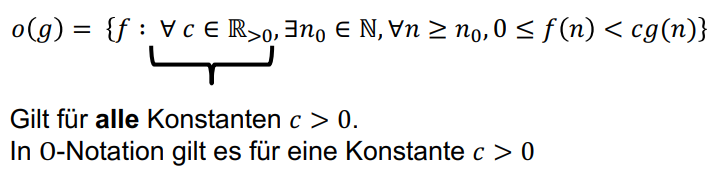
\includegraphics[width=12cm]{pictures/oKleinNotation.PNG}
                    $o(g)=\{f:\underbrace{\forall c \in \mathbb{R}_{>0}}_{
                        \mathclap{
                            \substack{
                                \text{Gilt für \fatsf{alle} Konstanten $c>0$.}\\
                                \text{In $\mathcal{O}$-Notation gilt es für eine Konstante $c>0$}}}
                        }, \exists n_0 \in \mathbb{N}, \forall n \geq n_0, 0\leq f(n)<cg(n)\}$
          \end{itemize}

    \item \textbf{$\omega$-Notation}
          \begin{itemize}
              \item $\omega$-Notation stellt eine echte untere Schranke dar
              \item Ausschlaggebend ist, dass es für alle $c \in \mathbb{R}{>0}$ gelten muss
              \item Au\ss erdem $>$ statt $\geq$
              \item z.B.: $\frac{n^2}{2} = \omega(n)$ und $\frac{n^2}{2} \neq \omega(n^2)$
              \item[] %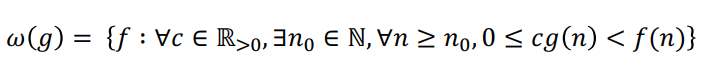
\includegraphics[width=12cm]{pictures/omegaKleinNotation.PNG}
                    $\omega(g)=\{f:\forall c \in \mathbb{R}_{>0},\exists n_0 \in \mathbb{N} \forall n \geq n_0,0\leq cg(n)<f(n)\}$
          \end{itemize}
\end{itemize}
\clearpage
\subsection{Insertion Sort \textmd{(Sortieren durch Einfügen)}}\label{InsertionSort}
\begin{itemize}
    \item \fatsf{Idee}
          \begin{itemize}
              \item Halte die linke Teilfolge sortiert
              \item Füge nächsten Schlüsselwert hinzu, indem es an die korrekte Position eingefügt wird
              \item Wiederhole den Vorgang bis Teilfolge aus der gesamten Liste besteht
          \end{itemize}

    \item \fatsf{Code}
          \begin{itemize}
              \begin{ccode}[autogobble]{title=Insertion-Sort(A)}
                  FOR j = 1 TO A.length - 1
                    key = A[j]
                    // Füge A[j] in die sortierte Sequenz A[0...j-1] ein
                    i = j - 1
                    WHILE i >= 0 and A[i] > key
                        A[i + 1] = A[i]
                        i = i - 1
                    A[i + 1] = key
              \end{ccode}
          \end{itemize}

    \item \fatsf{Schleifeninvariante von \texttt{Insertion Sort}}\label{insSortSiv}
          \begin{itemize}
              \item Zu Beginn jeder Iteration der \texttt{for}-Schleife besteht die Teilfolge \texttt{A[0...j-1]} aus den Elementen \\
                    der ursprünglichen Teilfolge \texttt{A[0...j-1]} enthaltenen Elementen, allerdings in sortierter Reihenfolge.
          \end{itemize}

    \item \fatsf{Korrektheit von \texttt{Insertion Sort}}
          \begin{itemize}
              \item \textit{Initialisierung:}
                    \begin{itemize}
                        \item   Beginn mit \texttt{j=1}, also Teilfeld \texttt{A[0...j-1]} besteht nur aus einem Element \texttt{A[0]}. \\
                              Dies ist auch das ursprüngliche Element und Teilfeld ist sortiert.
                    \end{itemize}

              \item \textit{Fortsetzung:}
                    \begin{itemize}
                        \item   Zu zeigen ist, dass die Invariante bei jeder Iteration erhalten bleibt. Ausführungsblock der \texttt{for}-Schleife
                              sorgt dafür, dass \texttt{A[j-1], A[j-2]},... je um Stelle nach rechts geschoben werden bis \texttt{A[j]} korrekt eingefügt wurde.
                              Teilfeld \texttt{A[0...j]} besteht aus ursprünglichen Elementen und ist sortiert. Inkrementieren von j erhält die Invariante.
                    \end{itemize}

              \item \textit{Terminierung: }
                    \begin{itemize}
                        \item   Abbruchbedingung der \texttt{for}-Schleife, wenn \texttt{j > A.length - 1}. Jede Iteration erhöht j.
                              Dann bei Abbruch ist \texttt{j = n } und einsetzen in Invariante liefert das Teilfeld \texttt{A[0...n-1]}
                              welches aus den ursprünglichen Elementen besteht und sortiert ist. Teilfeld ist gesamtes Feld.
                    \end{itemize}

              \item Algorithmus \texttt{Insertion Sort} arbeitet damit korrekt.

          \end{itemize}
          \clearpage
    \item \textbf{Laufzeitanalyse von \texttt{Insertion Sort}} {\label{insSortLaufzeit}}\\
          \vspace*{-1em}
          \begin{itemize}
              \item[]
                    \begin{minipage}{0.3\textwidth}
                        \centering
                        \renewcommand{\arraystretch}{.8}
                        \resizebox{\textwidth}{!}{%
                            \begin{tabular}{ccc}
                                \toprule
                                \fatsf{Zeile} & \fatsf{Kosten} & \fatsf{Anzahl}                         \\
                                \midrule
                                1             & $c_1$          & $n$                                    \\
                                2             & $c_2$          & $n-1$                                  \\
                                3             & $0$            & $n-1$                                  \\
                                4             & $c_4$          & $n-1$                                  \\
                                5             & $c_5$          & $\displaystyle\sum_{j=1}^{n-1}t_j$     \\
                                6             & $c_6$          & $\displaystyle\sum_{j=1}^{n-1}(t_j-1)$ \\
                                7             & $c_7$          & $\displaystyle\sum_{j=1}^{n-1}(t_j-1)$ \\
                                8             & $c_8$          & $n-1$                                  \\
                                \bottomrule
                            \end{tabular}}
                        %\caption{Laufzeitanalyse von Insertion-Sort}
                        \label{tab:insertion-sort:laufzeit}
                    \end{minipage}
                    \begin{minipage}[t]{0.45\textwidth}
                        \vspace*{-2.5cm}
                        \begin{itemize}
                            \item Festlegung der Laufzeit für jede Zeile
                            \item Jede Zeile besitzt gewissen Kosten \texttt{$c_i$}
                            \item Jede Zeile wird $x$ mal durchgeführt
                            \item $Laufzeit = Anzahl * Kosten$ jeder Zeile
                            \item Schleifen: Abbruchüberprüfung zählt auch
                            \item \texttt{$t_j$}: Anzahl der Abfragen der \texttt{While}-Schleife
                            \item Laufzeit:
                            $T(n)=c_{1} n+c_{2}(n-1)+c_{4}(n-1)+c_{5} \sum_{j=1}^{n-1} t_{j}+c_{6} \sum_{j=1}^{n-1}\left(t_{j}-1\right)$\\$+c_{7} \sum_{j=1}^{n-1}\left(t_{j}-1\right)+c_{8}(n-1)$
                        \end{itemize}
                    \end{minipage}
                    \vspace*{-1.1em}
              \item \textit{Warum $n$ in Zeile 1?}
                    \begin{itemize}
                        \item Die Überprüfung der Fortführungsbedingung beinhaltet auch die letze Überprüfung
                        \item Quasi die Überprüfung, durch die die Schleife abbricht
                    \end{itemize}

              \item \textit{Warum $\sum^{n-1}_{j=1}$ in Zeile 5?}
                    \begin{itemize}
                        \item Aufsummierung aller einzelnen $t_j$ über die Anzahl der Schleifendurchläufe
                        \item Diese ist allerdings $n-1$ und nicht $n$, da die Abbruchüberprüfung dort auch enthalten ist
                    \end{itemize}

              \item \textit{Warum $t_j-1$ in Zeile 6?}
                    \begin{itemize}
                        \item Selbes Argument wie oben, bei $t_j$ ist die Abbruchüberprüfung enthalten
                        \item Deswegen wird die \texttt{while}-Schleife nur $t_j-1$-mal ausgeführt
                    \end{itemize}

              \item \textit{\texttt{Best Case}}
                    \begin{itemize}
                        \item zu sortierendes Feld ist bereits sortiert
                        \item $t_j$ wird dadurch zu 1, da die \texttt{While}-Schleife immer nur einmal prüft (Abbruch)
                        \item Die zwei Zeilen innerhalb der \texttt{While}-Schleife werden nie ausgeführt
                        \item Durch Umformen ergibt sich, dass die Laufzeit eine lineare Funktion in $n$ ist
                    \end{itemize}

              \item \textit{\texttt{Worst Case}}
                    \begin{itemize}
                        \item zu sortierendes Feld ist umgekehrt sortiert
                        \item $t_j$ wird dadurch zu $j+1$, da die \texttt{While}-Schleife immer die gesamte Länge prüft
                        \item Durch Umformen ergibt sich, dass die Laufzeit eine quadratische Funktion in $n$ ist ($n^2$)
                    \end{itemize}

              \item \textit{\texttt{Average Case} }
                    \begin{itemize}
                        \item im Mittel gut gemischt
                        \item $t_j$ wird dadurch zu $j/2$
                        \item Die Laufzeit bleibt aber eine quadratische Funktion in $n$ ($n^2$)
                    \end{itemize}
          \end{itemize}

    \item \textbf{Asymptotische Laufzeitbetrachtung $\Theta$} {\label{insSortLaufzeitTheta}}
          \begin{itemize}
              \item $T(n)$ lässt sich als quadratische Funktion $an^2 + bn + c$ betrachten
              \item Terme niedriger Ordnung sind für gro\ss e $n$ irrelevant
              \item Deswegen Vereinfachung zu $n^2$ und damit $\Theta(n^2)$
          \end{itemize}
\end{itemize}
\clearpage
\subsection{Bubble Sort}\label{BubbleSort}
\begin{itemize}
    \item \fatsf{Idee}
          \begin{itemize}
              \item Vergleiche Paare von benachbarten Schlüsselwerten
              \item Tausche das Paar, falls rechter Schlüsselwert kleiner als linker
          \end{itemize}

    \item \fatsf{Code}
          \begin{itemize}
              \item[]
                    \begin{ccode}[autogobble]{title=BubbleSort(A)}
                        FOR i = 0 TO A.length - 2
                            FOR j = A.length - 1 DOWNTO i + 1
                                IF A[j] < A[j-1]
                                    SWAP(A[j], A[j-1])
                    \end{ccode}
          \end{itemize}

    \item \fatsf{Analyse von \texttt{Bubble Sort}}
          \begin{itemize}
              \item \textit{Anzahl der Vergleiche:}
                    \begin{itemize}
                        \item Es werden stets alle Elemente der Teilfolge miteinander verglichen
                        \item Unabhängig von der Vorsortierung sind \texttt{Worst} und \texttt{Best Case} identisch
                    \end{itemize}

              \item \textit{Anzahl der Vertauschungen:}
                    \begin{itemize}
                        \item \texttt{Best Case}: 0 Vertauschungen
                        \item \texttt{Worst Case}: $\frac{n^2-n}{2}$ Vertauschungen
                    \end{itemize}

              \item \textit{Komplexität:}
                    \begin{itemize}
                        \item \texttt{Best Case}: $\Theta(n)$
                        \item \texttt{Average Case}: $\Theta(n^2)$
                        \item \texttt{Worst Case}: $\Theta(n^2)$
                    \end{itemize}
          \end{itemize}

\end{itemize}
\clearpage
\subsection{Selection Sort}\label{Selection sort}
\begin{itemize}
    \item \fatsf{Idee}
          \begin{itemize}
              \item Sortieren durch direktes Auswählen
              \item \texttt{MinSort}: "wähle kleines Element in Array und tausche es nach vorne"
              \item \texttt{MaxSort}: "wähle größtes Element in Array und tausche es nach vorne"
          \end{itemize}

    \item \fatsf{Code - MinSort}
          \begin{itemize}
              \item[]
                    \begin{ccode}[autogobble]{title=Selection-Sort(A)}
                        FOR i = 0 TO A.length - 2
                            k = i
                            FOR j = i + 1 TO A.length - 1
                                IF A[j] < A[k]
                                    k = j
                            SWAP(A[i], A[k])
                    \end{ccode}
          \end{itemize}
\end{itemize}

%\pagebreak
\subsection{Divide-And-Conquer Prinzip}\label{Divide-And-Conquer}
\begin{itemize}
    \item Anderer Ansatz im Gegensatz zu z.B. \texttt{InsertionSort} (inkrementelle Herangehensweise)
    \item Laufzeit ist im schlechtesten Fall immer noch besser als \texttt{InsertionSort}
    \item Prinzip: Zerlege das Problem und löse es direkt oder zerlege es weiter
    \item \textit{Divide:}
          \begin{itemize}
              \item Teile das Problem in mehrere Teilprobleme auf
              \item Teilprobleme sind Instanzen des gleichen Problems
          \end{itemize}
    \item \textit{Conquer:}
          \begin{itemize}
              \item Beherrsche die Teilprobleme rekursiv
              \item Falls Teilprobleme klein genug, löse sie auf direktem Weg
          \end{itemize}
    \item \textit{Combine:}
          \begin{itemize}
              \item Vereine die Lösungen der Teilprobleme zu Lösung des ursprünglichen Problems
          \end{itemize}
\end{itemize}
\clearpage
\subsection{Merge Sort} \label{Merge Sort}
\begin{itemize}
    \item \fatsf{Idee}
          \begin{itemize}
              \item \textit{Divide:} Teile die Folge aus $n$ Elementen in zwei Teilfolgen von je $\frac{n}{2}$ Elemente auf
              \item \textit{Conquer:} Sortiere die zwei Teilfolgen rekursiv mithilfe von \texttt{MergeSort}
              \item \textit{Combine:} Vereinige die zwei sortierten Teilfolgen, um die sortierte Lösung zu erzeugen
          \end{itemize}
    \item \fatsf{Code}
          \begin{ccode}[autogobble,escapeinside=||]{title={MERGE-SORT(A,p,r)}}
              IF p < r
                q = |$\left \lfloor \texttt{(p+r)/2} \right \rfloor$| // Teilen in 2 Teilfolgen
                MERGE-SORT(A,p,q) // Sortieren der beiden Teilfolgen
                MERGE-SORT(A,q+1,r)
                MERGE(A,p,q,r) // Vereinigung der beiden sortierten Teilfolgen
          \end{ccode}
          \begin{ccode}[autogobble,escapeinside=||]{title={MERGE(A,p,q,r)}}
              |$n_1$| = q - p + 1
              |$n_2$| = r - q
              Let L[0...|$n_1$|] and R[0...|$n_2$|] be new arrays
              FOR i = 0 TO |$n_1$| - 1 // Auffüllen der neu erstellten Arrays
                L[i] = A[p + i]
              FOR j = 0 TO |$n_2$| - 1
                R[j] = A[q + j + 1]
              L[|$n_1$|] = |$\infty$| // Einfügen des Sentinel-Wertes
              R[|$n_2$|] = |$\infty$|
              i = 0
              j = 0
              FOR k = p TO r  // Eintragweiser Vergleich der Elemente
                IF L[i] |$\leq$| R[j]
                    A[k] = L[i] // Sortiertes Zurückschreiben in Original-Array
                    i = i + 1
                ELSE
                    A[k] = R[j]
                    j = j + 1
          \end{ccode}
          (Teilarrays werden nicht parallel bearbeitet)
    \item \fatsf{Korrektheit von MergeSort}
          \begin{itemize}
              \item \textit{Schleifeninvariante}
                    \begin{itemize}
                        \item[]
                              Zu Beginn jeder Iteration der \texttt{for}-Schleife (Letztes \texttt{for} in Methode \texttt{MERGE}) enthält
                              das Teilfeld \texttt{A[p...k-1]} die \texttt{k-p} kleinsten Elemente aus \texttt{L[0...$n_1$]} und \texttt{R[0...$n_2$]}
                              in sortierter Reihenfolge. Weiter sind \texttt{L[i]} und \texttt{R[i]} die kleinsten Elemente ihrer Arrays, die noch nicht
                              zurück kopiert wurden.
                    \end{itemize}
              \item \textit{Initialisierung}
                    \begin{itemize}
                        \item[]
                              Vor der ersten Iteration gilt \texttt{k=p}. Daher ist \texttt{A[p...k-1]} leer und enthält 0 kleinste Elemente von
                              \texttt{L} und \texttt{R}. Wegen \texttt{i=j=0} sind \texttt{L[i]} und \texttt{R[i]} die kleinsten Elemente ihrer
                              Arrays, die noch nicht zurück kopiert wurden.
                    \end{itemize}
                    \clearpage
              \item \textit{Fortsetzung}
                    \begin{itemize}
                        \item[]
                              Müssen zeigen, dass Schleifeninvariante erhalten bleibt. Dafür nehmen wir an, dass \texttt{L[i] $\leq$ R[j]}. Dann ist
                              \texttt{L[i]} kleinstes Element, welches noch nicht zurück kopiert wurde. Da Array \texttt{A[p...k-1]} die \texttt{k-p}
                              kleinsten Elemente enthält, wird der Array \texttt{A[p...k]} die \texttt{k-p+1} kleinsten Elemente enthalten, nachdem
                              der Wert nach der Durchführung von \texttt{A[k]=L[i]} kopiert wurde. Die Erhöhung der Variablen \texttt{k} und \texttt{i}
                              stellt die Schleifeninvariante für die nächste Iteration wieder her. Wenn \texttt{L[i]>R[j]} dann analoges Argument
                              in der \texttt{ELSE}-Anweisung.
                    \end{itemize}
              \item \textit{Terminierung}
                    \begin{itemize}
                        \item[]
                              Beim Abbruch gilt \texttt{k=r+1}. Durch die Schleifeninvariante enthält \texttt{A[p...r]} die kleinste Elemente von
                              \texttt{L[0...$n_1$]} und \texttt{R[0...$n_2$]} in sortierter Reihenfolge. Alle Elemente außer der Sentinels wurden
                              komplett zurück kopiert. \texttt{MergeSort} ist außerdem ein stabiler Algorithmus.
                    \end{itemize}
          \end{itemize}

    \item \fatsf{Analyse von MergeSort}
          \begin{itemize}
              \item Ziel: Bestimme Rekursionsgleichung für Laufzeit $T(n)$ von $n$ Zahlen im schlechtesten Fall
              \item Divide: Berechnung der Mitte des Feldes: Konstante Zeit $\Theta(1)$
              \item Conquer: Rekursives Lösen von zwei Teilproblemen der Größe $\frac{n}{2}$: Laufzeit von $2~T(\frac{n}{2})$
              \item Combine: \texttt{MERGE} auf einem Teilfeld der Länge $n$: Lineare Zeit $\Theta(n)$
              \item[] \[
                        T(n) = \left.
                        \begin{cases}
                            \Theta(1)                    & \text{falls } n = 1 \\
                            2~T(\frac{n}{2}) + \Theta(n) & \text{falls } n > 1 \\
                        \end{cases}
                        \right \}
                    \]
              \item Lösen der Rekursionsgleichung mithilfe eines Rekursionsbaums
                    \begin{itemize}
                        \item[] 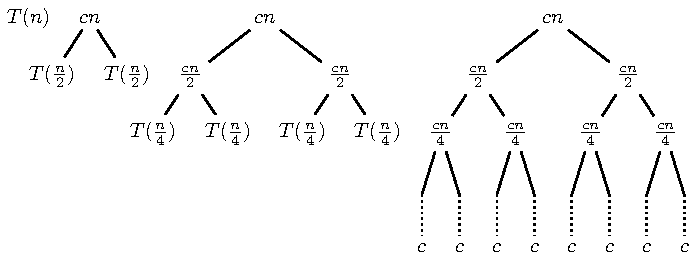
\includegraphics[width=14cm]{pictures/merge_sort_equation/merge_sort_equation}
                        \item Verwenden der Konstante $c$ statt $\Theta(1)$
                        \item $cn$ stellt den Aufwand an der ersten Ebene dar
                        \item Der addierte Aufwand jeder Stufe (aller Knoten) ist auch $cn$
                        \item Die Azahl der Ebenen lässt sich mithilfe von $lg(n) + 1$ bestimmen (2-er Logarithmus)
                        \item Damit ergibt sich für die Laufzeit: $cn \cdot lg(n)+cn$
                        \item Für $\lim_{n \rightarrow \infty}$ wird diese zu $n \cdot lg(n)$
                        \item Laufzeit beträgt damit $\Theta(n \cdot lg(n))$
                        \item Laufzeit von \texttt{MergeSort} ist in jedem Fall gleich
                    \end{itemize}

          \end{itemize}
\end{itemize}
\clearpage
\subsection{Quicksort}\label{Quicksort}
\begin{itemize}
    \item \fatsf{Idee}
          \begin{itemize}
              \item \textit{Pivotelement:}
                    \begin{itemize}
                        \item[]
                              Wahl eines Pivotelement \texttt{x} aus dem Array
                    \end{itemize}

              \item \textit{Divide:}
                    \begin{itemize}
                        \item[]
                              Zerlege den Array \texttt{A[p...r]} in zwei Teilarrays \texttt{A[p...q-1]} und \texttt{A[q+1...r]},
                              sodass jedes Element von \texttt{A[p...q-1]} kleiner oder gleich \texttt{A[q]} ist, welches
                              wiederum kleiner oder gleich jedem Element von \texttt{A[q+1...r]} ist. Berechnen Sie den Index \texttt{q}
                              als Teil vom \texttt{Partition} Algorithmus.
                    \end{itemize}

              \item \textit{Conquer:}
                    \begin{itemize}
                        \item[]
                              Sortieren beider Teilarrays \texttt{A[p...q-1]} und \texttt{A[q+1...r]} durch rekursiven Aufruf von
                              Quicksort.
                    \end{itemize}

              \item \textit{Combine:}
                    \begin{itemize}
                        \item[]
                              Da die Teilarrays bereits sortiert sind, ist keine weitere Arbeit nötig um diese zu vereinigen.
                              \texttt{A[p$\ldots$r]} ist nun sortiert.
                    \end{itemize}
          \end{itemize}

    \item \fatsf{Code}
          \begin{ccode}[autogobble,escapeinside=||]{title={QUICKSORT(A,p,r)}}
              IF p < r    // Überprüfung, ob Teilarray leer ist
                q = PARTITION(A,p,r)
                QUICKSORT(A,p,q-1)
                QUICKSORT(A,q+1,r)
          \end{ccode}
          \begin{ccode}[autogobble,escapeinside=||]{title={PARTITION(A,p,r)}}
              x = A[r]    // Wahl des Pivotelements
              i = p - 1   // Index i setzen
              FOR j = p TO r - 1 // Auffüllen des Teilarrays mit Elementen
                IF A[j] |$\leq$| x
                    i = i + 1
                    SWAP(A[i], A[j])
              SWAP(A[i+1], A[r]) // Tausch des Pivotelements
              RETURN i + 1 // Neuer Index des Pivotelements
          \end{ccode}
          (Teilarrays werden nicht parallel bearbeitet)
          \clearpage
    \item \fatsf{Korrektheit von Quicksort}
          \begin{itemize}
              \item \textit{Schleifeninvariante:}
                    \begin{itemize}
                        \item[]
                              Zu Beginn jeder Iteration der \texttt{for}-Schleife gilt für den Arrayindex $k$ folgendes:
                              \begin{enumerate}
                                  \item Ist $p \leq k \leq i$, so gilt \texttt{A[k]} $\leq x$
                                  \item Ist $i+1 \leq k \leq j -1$, so gilt \texttt{A[k]} $> x$
                                  \item Ist $k = r$, so gilt \texttt{A[k]} $= x$
                              \end{enumerate}
                    \end{itemize}

              \item \textit{Initialisierung:}
                    \begin{itemize}
                        \item[]
                              Vor der ersten Iteration gilt $i = p - 1$ und $j = p$. Da es keine Werte zwischen $p$ und $j$
                              gibt und es auch keine Werte zwischen $i + 1$ und $j - 1$ gibt, sind die ersten beiden Eigenschaften
                              trivial erfüllt. Die Zuweisung in \texttt{x = A[r]} sorgt für die Erfüllung der dritten Eigenschaft.
                    \end{itemize}

              \item \textit{Fortsetzung:}
                    \begin{itemize}
                        \item[]
                              Zwei mögliche Fälle durch \texttt{IF A[j] $\leq$ x}. Wenn \texttt{A[j] > x}, dann inkrementiert die
                              Schleife nur den Index $j$. Dann gilt Bedingung 2 für \texttt{A[j-1]} und alle anderen Einträge
                              bleiben unverändert. Wenn \texttt{A[j] $\leq$ x}, dann wird Index $i$ inkrementiert und die
                              Einträge \texttt{A[i]} und \texttt{A[j]} getauscht und schließlich der Index $j$ erhöht. Wegen
                              des Vertauschens gilt \texttt{A[i] $\leq$ x} und Bedingung 1 ist erfüllt. Analog gilt
                              \texttt{A[j-1] > x}, da das Element welches mit \texttt{A[j-1]} vertauscht wurde wegen der
                              Invariante gerade größer als $x$ ist.
                    \end{itemize}

              \item \textit{Terminierung:}
                    \begin{itemize}
                        \item[]
                              Bei der Terminierung gilt, dass $j = r$. Daher gilt, dass jeder Eintrag des Arrays zu einer der drei
                              durch die Invariante beschriebenen Mengen gehört.
                    \end{itemize}
          \end{itemize}

    \item \textbf{Performanz von Quicksort}
          \begin{itemize}
              \item \textit{Abhängig von der \textbf{Balanciertheit} der Teilarrays}
                    \begin{itemize}
                        \item Definition Balanciert: ungefähr gleiche Anzahl an Elementen
                        \item Teilarrays balanciert: Laufzeit asymptotisch so schnell wie \texttt{MergeSort}
                        \item Teilarrays unbalanciert: Laufzeit kann so langsam wie \texttt{InsertionSort} laufen
                    \end{itemize}

              \item \textit{Zerlegung im \textbf{schlechtesten Fall}}
                    \begin{itemize}
                        \item Partition zerlegt Problem in ein Teilproblem mit $n-1$ Elementen und eins mit $0$ Elementen
                        \item Unbalancierte Zerlegung mit Kosten $\Theta(n)$ zieht sich durch gesamte Rekursion
                        \item Aufruf auf Feld der Größe 0: $T() = \Theta(1)$
                        \item Laufzeit (rekursiv):
                              \begin{itemize}
                                  \item $T(n) = T(n-1) + T(0) + \Theta(n) = T(n-1) + \Theta(n)$
                                  \item Insgesamt folgt: $T(n) = \Theta(n^2)$
                              \end{itemize}
                    \end{itemize}

              \item \textit{Zerlegung im \textbf{besten Fall}}
                    \begin{itemize}
                        \item Problem wird so balanciert wie möglich zerlegt
                        \item Zwei Teilprobleme mit maximaler Größe von $\frac{n}{2}$
                        \item Zerlegung kostet $\Theta(n)$
                        \item Laufzeit (rekursiv):
                              \begin{itemize}
                                  \item $T(n) \leq 2T(\frac{n}{2}) + \Theta(n)$
                                  \item Laufzeit beträgt: $O(n~lg(n))$
                              \end{itemize}
                        \item Solange die Aufteilung konstant bleibt, bleibt die Laufzeit $O(n~lg(n))$
                    \end{itemize}

          \end{itemize}
\end{itemize}
\clearpage

\subsection{Laufzeitanalyse von rekursiven Algorithmen}\label{Laufzeit rekursive Algorithmen}
\begin{itemize}
    \item \fatsf{Analyse von Divide-And-Conquer Algorithmen}
          \begin{itemize}
              \item $T(n)$ ist Laufzeit eines Problems der Größe $n$
              \item Für kleines Problem benötigt die direkte Lösung eine konstante Zeit $\Theta(1)$
              \item Für sonstige $n$ gilt:
                    \begin{itemize}
                        \item Aufteilen eines Problems führt zu $a$ Teilproblemen
                        \item Jedes dieser Teilprobleme hat die Größe $\frac{1}{b}$ der Größe des ursprünglichen Problems
                        \item Lösen eines Teilproblems der Größe $\frac{n}{b}$: $T(\frac{n}{b})$
                        \item Lösen $a$ solcher Probleme: $a~T(\frac{n}{b})$
                        \item $D(n)$: Zeit um das Problem aufzuteilen (Divide)
                        \item $C(n)$: Zeit um Teillösungen zur Gesamtlösung zusammenzufügen (Combine)
                        \item[] \[
                                  T(n) = \left.
                                  \begin{cases}
                                      \Theta(1)                      & \text{falls } n \leq c \\
                                      a~T(\frac{n}{b}) + D(n) + C(n) & \text{sonst}           \\
                                  \end{cases}
                                  \right \}
                              \]
                    \end{itemize}
          \end{itemize}

    \item \fatsf{Subsitutionsmethode}
          \begin{itemize}
              \item Idee: Erraten einer Schranke und Nutzen von Induktion zum Beweis der Korrektheit
              \item Ablauf:
                    \begin{enumerate}
                        \item Rate die Form der Lösung (Scharfes Hinsehen oder kurze Eingaben ausprobieren/einsetzen)
                        \item Anwendung von vollständiger Induktion zum Finden der Konstanten und Beweis der Lösung
                    \end{enumerate}
                    \clearpage
              \item \fatsf{Beispiel}
                    \begin{itemize}
                        \item \textit{Betrachten von \texttt{MergeSort}:}
                              \begin{itemize}
                                  \item $T(1) \leq c$
                                  \item $T(n) \leq T(\left \lfloor \frac{n}{2} \right \rfloor) + T(\left \lceil \frac{n}{2} \right \rceil) + cn$
                              \end{itemize}

                        \item \textit{Ziel:}
                              \begin{itemize}
                                  \item[]
                                        Obere Abschätzung $T(n) \leq g(n)$ mit $g(n)$ ist eine Funktion, die durch eine
                                        geschlossene Formel dargestellt werden kann.
                                  \item[]
                                        Wir \string"raten\string": $T(n) \leq 4cn~lg(n)$ und nehmen dies für alle $n' < n$ an und
                                        zeigen es für $n$.
                              \end{itemize}

                        \item \textit{Induktion:}
                              \begin{itemize}
                                  \item $lg$ steht hier für $\log_2$
                                  \item $n = 1$: $T(1) \leq c$
                                  \item {\makebox[2cm][l]{$n = 2$: $T(2)$}}  $\leq T(1) + T(1) +2c$
                                  \item[] {\makebox[2cm][l]{}} $\leq 4c \leq 8c$
                                  \item[] {\makebox[1cm][l]{}} $T(2) = 4c * 2~lg(2) = 8c$
                              \end{itemize}
                              %\clearpage
                        \item \textit{Hilfsbehauptungen:}
                              \begin{itemize}
                                  \item (1): $\left \lfloor \frac{n}{2} \right \rfloor + \left \lceil \frac{n}{2} \right \rceil = n$
                                  \item (2): $\left \lfloor \frac{n}{2} \right \rfloor \leq \frac{n}{2} \leq \frac{2}{3}n$
                                  \item (3): $\log_c(\frac{a}{b}) = \log_c(a) - \log_c(b)$
                                  \item (4): $\log_c(a*b) = \log_c(a) + \log_c(b)$
                              \end{itemize}
                        \item \textit{Induktionsschritt:}
                              \begin{itemize}
                                  \item Annahme: $n > 2$ und sei Behauptung wahr für alle $n' < n$.
                                  \item[]
                                        ${\makebox[1cm][l]{T(n)}}  \leq T(\left \lfloor \frac{n}{2} \right \rfloor) + T(\left \lceil \frac{n}{2} \right \rceil) + cn \\
                                            {\makebox[1cm][l]{}} \leq 4c \left \lfloor \frac{n}{2} \right \rfloor~ lg(\left \lfloor \frac{n}{2} \right \rfloor )
                                            + 4c \left \lceil \frac{n}{2} \right \rceil~ lg(\left \lceil \frac{n}{2} \right \rceil ) + cn \\
                                            {\makebox[1cm][l]{(HB)}} \leq 4c \cdot lg(\frac{2}{3}n) \cdot (\left \lfloor \frac{n}{2} \right \rfloor + \left \lceil \frac{n}{2} \right \rceil +cn \\
                                            {\makebox[1cm][l]{}} \leq 4c \cdot lg(\frac{2}{3}n) \cdot n + cn \\
                                            {\makebox[1cm][l]{(HB)}} \leq 4cn \cdot (lg(\frac{2}{3}) + lg(n)) + cn \\
                                            {\makebox[1cm][l]{}} = 4cn \cdot lg(n) + 4cn \cdot lg(\frac{2}{3}) \\
                                            {\makebox[1cm][l]{}} = 4cn \cdot lg(n) + cn (1+ 4 \cdot (lg(2) - lg(3))) \\
                                            {\makebox[1cm][l]{}} \leq 4cn \cdot lg(n) \\
                                            {\makebox[1cm][l]{}} \Rightarrow \Theta(n~lg(n))$
                              \end{itemize}
                    \end{itemize}
          \end{itemize}


    \item \fatsf{Rekursionsbaum}
          \begin{itemize}
              \item Idee: Stellen das Ineinander-Einsetzen als Baum dar und Analyse der Kosten
              \item Ablauf:
                    \begin{enumerate}
                        \item Jeder Knoten stellt die Kosten eines Teilproblems dar
                              \begin{itemize}
                                  \item Die Wurzel stellt die zu analysierenden Kosten $T(n)$ dar
                                  \item Die Blätter stellen die Kosten der Basisfälle dar (z.B. $T(0)$)
                              \end{itemize}
                        \item Berechnen der Kosten innerhalb jeder Ebene des Baums
                        \item Die Gesamtkosten sind die Summe über die Kosten aller Ebenen
                    \end{enumerate}
              \item Rekursionsbaum ist nützlich um Lösung für Subsitutionsmethode zu erraten
                    \clearpage
              \item \textbf{Beispiel:} $T(n) = 3T(\left \lfloor \frac{n}{4} \right \rfloor) + \Theta(n^2)$
                    \begin{itemize}
                        \item \textit{Vorüberlegungen:}
                              \begin{itemize}
                                  \item $\Rightarrow T(n) = 3T(\frac{n}{4}) + cn^2$ ($c>0$)
                                  \item Je Abstieg verringert sich die Größe des Problems um den Faktor 4.
                                  \item Erreichen der Randbedingung ist vonnöten, die Frage ist wann dies geschieht.
                                  \item Größe Teilproblem bei Level $i$: $\frac{n}{4^i}$
                                  \item Erreichen Teilproblem der Größe 1, wenn $\frac{n}{4^i}=1$, d.h. wenn $i=log_4(n)$ \\
                                        $\Rightarrow$ Baum hat also $\log_4n + 1$ Ebenen
                              \end{itemize}
                        \item \textit{Kosten pro Ebene:}
                              \begin{itemize}
                                  \item Jede Ebene hat 3-mal soviele Knoten wie darüber liegende
                                  \item Anzahl der Knoten in Tiefe $i$ ist $3^i$
                                  \item Kosten $c(\frac{n}{4^i})^2~,~i=0,\cdots, \log_4n-1$
                                  \item Anzahl $\cdot$ Kosten = $3^i \cdot c(\frac{n}{4^i})^2 = (\frac{3}{16})^i \cdot cn^2$
                              \end{itemize}
                              %\clearpage
                        \item \textit{Unterste Ebene:}
                              \begin{itemize}
                                  \item $3^{\log_4(n)} = n  {\log_4(3)}$ Knoten
                                  \item Jeder Knoten trägt $T(1)$ Kosten bei
                                  \item Kosten unten: $n^{\log_4(3)} \cdot T(1) = \Theta(n^{\log_4(3)})$
                              \end{itemize}
                        \item \textit{Addiere alle Kosten aller Ebenen:}
                              \begin{itemize}
                                  \item {\makebox[0.75cm][l]{$T(n)$}} $= cn^2 + \frac{3}{16}cn^2 + (\frac{3}{16})^2cn^2+...+ (\frac{3}{16})^{\log_4n-1}cn^2 + \Theta(n^{\log_4(3)})$
                                  \item[] {\makebox[0.75cm][l]{}} $= \sum^{\log_4n-1}_{i=0} (\frac{3}{16})^icn^2+ \Theta(n^{\log_4^3})$
                                  \item[] {\makebox[0.75cm][l]{}} $= \frac{(\frac{3}{16}^{\log_4n})-1}{\frac{3}{16}-1} \cdot cn^2 + \Theta(n^{\log_43})$ (Verwendung der geometrischen Reihe)
                                  \item Verwendung einer unendlichen fallenden geometrischen Reihe als obere Schranke:
                                  \item[] {\makebox[0.73cm][l]{$T(n)$}}  $= \sum^{\-1}_{i=0} (\frac{3}{16})^i \cdot cn^2 + \Theta(n^{\log_43})$
                                  \item[] {\makebox[0.73cm][l]{}} $< \sum^{\infty}_{i=0} (\frac{3}{16})^i \cdot cn^2 + \Theta(n^{\log_43})$
                                  \item[] {\makebox[0.75cm][l]{}} $= \frac{1}{1-\frac{3}{16}} \cdot cn^2 + \Theta(n^{\log_43})$
                                  \item[] {\makebox[0.75cm][l]{}} $ = \frac{16}{13} \cdot cn^2 + Theta(n^{\log_43}) = O(n^2)$
                              \end{itemize}
                        \item \textit{Jetzt \textbf{Subsitutionsmethode:}}
                              \begin{itemize}
                                  \item Zu zeigen: $\exists d > 0: T(n) \leq dn^2$
                                  \item Induktionsanfang:
                                  \item[] {\makebox[0.75cm][l]{$T(n)$}} $= 3 \cdot T(\left \lfloor \frac{1}{4} \right \rfloor) + c \cdot 1^2$
                                  \item[] {\makebox[0.75cm][l]{}} $= 3 \cdot T(0) + c = c$
                                  \item Induktionsschritt:
                                  \item[] {\makebox[0.75cm][l]{$T(n)$}} $\leq 3 \cdot T(\left \lfloor \frac{n}{4} \right \rfloor) + cn^2$
                                  \item[] {\makebox[0.75cm][l]{}} $\leq 3 \cdot d(\left \lfloor \frac{n}{4} \right \rfloor)^2+cn^2$
                                  \item[] {\makebox[0.75cm][l]{}} $\leq 3d(\frac{n}{4})^2 + cn^2$
                                  \item[] {\makebox[0.75cm][l]{}} $= \frac{3}{16}dn^2+cn^2$
                                  \item[] {\makebox[0.75cm][l]{}} $\leq dn^2$, falls $d \geq \frac{16}{13}c$
                              \end{itemize}

                    \end{itemize}
          \end{itemize}

    \item \fatsf{Mastertheorem}
          \begin{itemize}
              \item \textit{Idee:}
                    \begin{itemize}
                        \item[]
                              Seien $a \geq 1$ und $b > 1$ Konstanten. Sei $f(n)$ eine positive Funktion und $T(n)$
                              über den nichtnegativen ganzen Zahlen über die Rekursionsgleichung $T(n) = a~T(\frac{n}{b}) + f(n)$
                              defininiert, wobei wir $\frac{n}{b}$ so interpretieren, dass damit entweder $\left \lfloor \frac{n}{b} \right \rfloor$
                              oder $\left \lceil \frac{n}{b} \right \rceil$ gemeint ist. Dann besitzt $T(n)$ die folgenden asymptotischen Schranken
                              ($a$ und $b$ werden aus $f(n)$ gelesen):
                              \begin{enumerate}
                                  \item Gilt $f(n) = O(n^{\log_b (a - \epsilon)})$ für eine Konstante $\epsilon > 0$, dann $T(n) = \Theta(n^{\log_b (a)})$
                                  \item Gilt $f(n) = \Theta(n^{\log_b (a)})$, dann gilt $T(n) = \Theta(n^{\log_b (a)} lg(n))$
                                  \item Gilt $f(n) = \Omega(n^{\log_b (a+\epsilon)})$ für eine Konstante $\epsilon > 0$ und $a~f(\frac{n}{b}) \leq c~f(n)$
                                        für eine \\ Konstante $c < 1$ und hinreichend großen $n$, dann ist $T(n) = \Theta(f(n))$
                              \end{enumerate}
                    \end{itemize}

              \item \textit{Erklärung:}
                    \begin{itemize}
                        \item In jedem der 3 Fälle wird die Funktion $f(n)$ mit $n^{\log_b(a)}$ verglichen
                              \begin{enumerate}
                                  \item Wenn $f(n)$ polynomial kleiner ist als $n^{\log_b(a)}$, dann $T(n) = \Theta(n^{\log_b(a)})$
                                  \item Wenn $f(n)$ und $n^{\log_b(a)}$ die gleiche Größe haben, gilt $T(n) = \Theta(n^{\log_b (a)} lg(n))$
                                  \item Wenn $f(n)$ polynomial größer als $n^{\log_b(a)}$ und $a~f(\frac{n}{b}) \leq c~f(n)$ erfüllt, dann $T(n) = \Theta(f(n))$
                              \end{enumerate}
                        \item (polynomial größer/kleiner: um Faktor $n^\epsilon$ asymptotisch größer/kleiner)
                    \end{itemize}

              \item \textit{Nicht abgedeckte Fälle:}
                    \begin{itemize}
                        \item Wenn einer dieser Fälle eintritt, kann das Mastertheorem nicht angewendet werden
                              \begin{enumerate}
                                  \item Wenn $f(n)$ kleiner ist als $n^{\log_b(a)}$, aber nicht polynomial kleiner
                                  \item Wenn $f(n)$ größer ist als $n^{\log_b(a)}$, aber nicht polynomial größer
                                  \item Regularitätsbedingung $a~f(\frac{n}{b}) \leq c~f(n)$ wird nicht erfüllt
                                  \item $a$ oder $b$ sind nicht konstant (z.B. $a=2^n$)
                              \end{enumerate}
                    \end{itemize}
                    \clearpage
              \item \textit{Beispiel:}
                    \begin{itemize}
                        \item \textit{$T(n) = 9T(\frac{n}{3}) + n$}
                              \begin{itemize}
                                  \item $a=9, b=3, f(n)=n$
                                  \item $\log_b(a) = \log_3(9) = 2$
                                  \item {\makebox[1.5cm][l]{$f(n) = n$}} $= O(n^{\log_b(a-\epsilon)})$
                                  \item[] {\makebox[1.5cm][l]{}} $= O(n^{2-\epsilon})$
                                  \item Ist diese Gleichung für ein $\epsilon > 0$ erfüllt? $\Rightarrow$ $\epsilon = 1$
                                  \item \fatsf{1. Fall} $\Rightarrow$ $T(n) = \Theta(n^2)$
                              \end{itemize}

                        \item \textit{$T(n) = T(\frac{2n}{3}) + 1$}
                              \begin{itemize}
                                  \item $a=1, b= \frac{3}{2}, f(n) = 1$
                                  \item $\log_{\frac{3}{2}} 1 = 0$
                                  \item {\makebox[1.5cm][l]{$f(n) = 1$}} $= O(n^{\log_b(a)})$
                                  \item[] {\makebox[1.5cm][l]{}} $= O(n^0)$
                                  \item[] {\makebox[1.5cm][l]{}} $= O(1)$
                                  \item \fatsf{2.Fall} $\Rightarrow$ $T(n) = \Theta(1 * lg(n)) = \Theta(lg(n))$
                              \end{itemize}

                        \item \textit{$T(n) = 3(T\frac{n}{4}) + n~lg(n)$}
                              \begin{itemize}
                                  \item $a=3,b=4,f(n)= n~lg(n)$
                                  \item $n^{\log_b(a)} = n^{\log_4(3)} \leq n^{0.793}$
                                  \item $\epsilon = 0.1$ im Folgenden
                                  \item $f(n) = n~lg(n) \geq n \geq n^{0.793 + 0.1} \geq n^{0.793}$
                                  \item \fatsf{3.Fall} $\Rightarrow$ $f(n) = \Omega(n^{\log_b(a+0.1)})$
                                  \item $a f(\frac{n}{b}) = 3f(\frac{n}{4}) = 3(\frac{n}{4})~lg(\frac{n}{4}) \leq \frac{3}{4} n~lg(n)$
                                  \item Damit ist auch die Randbedingung erfüllt und $T(n) = \Theta(n~lg(n))$

                              \end{itemize}
                    \end{itemize}
          \end{itemize}

\end{itemize}
%Horizontal Seperator
\hbox to \hsize{\cleaders\hbox to 1em{-}\hfill\hfil}
\vspace{3cm}
\begin{table}[ht]
    \centering
    \begin{tabular}{c|c|c}
        \fatsf{Grundlegende Datenstrukturen}            & \fatsf{Fortgeschrittene Datenstrukturen}         & \fatsf{Randomisierte Datenstrukturen} \\
        \toprule
        \hyperref[Stacks]{Stacks}                       & \hyperref[Rot-Schwarz-Baeume]{Rot-Schwarz-Bäume} & \hyperref[Skip Lists]{Skip Lists}     \\
        \hyperref[Verkettete Listen]{Verkettete Listen} & \hyperref[AVL-Baeume]{AVL-Bäume}                 & \hyperref[Hashtables]{Hash Tables}    \\
        \hyperref[Queues]{Queues}                       & \hyperref[Splay-Baeume]{Splay-Bäume}             & \hyperref[Bloom-Filter]{Bloom-Filter} \\
        \hyperref[Binaere Baeume]{Bäume}                & \hyperref[Binaere Max-Heaps]{Heaps}              &                                       \\
        \hyperref[Binaere Suchbaeume]{Binäre Suchbäume} & \hyperref[B-Baeume]{B-Bäume}                     &                                       \\
    \end{tabular}
    \caption{Übersicht Datenstrukturen}
    \label{tab:overview_dataStructures}
\end{table}
\clearpage
\end{document}
\documentclass[
    12pt,
    a4paper,
    ngerman,
    color=3b,% Farbe für Hervorhebungen auf Basis der Deklarationen in den
    %type=intern,
    %titlepage=true,
    marginpar=false,
    colorback=false,
    %logo=head,
    leqno,
]{tudaexercise}
\usepackage{import}
% Import all Packages from Main Preamble with relative Path
\subimport*{../../}{preamble}
% Get Labels from Main Document using the xr-hyper Package
\externaldocument{../../AuD-Zusammenfassung-2020}
% Set Graphics Path, so pictures load correctly
\graphicspath{{../../}}


\begin{document}
\section{Grundlegende Datenstrukturen}
\subsection{Stacks}\label{Stacks}
\begin{itemize}
    \item \fatsf{Abstrakter Datentyp Stack}
          \begin{itemize}
              \item \texttt{new S()}
                    \begin{itemize}
                        \item Erzeugt neuen (leeren) Stack
                    \end{itemize}
              \item \texttt{s.isEmpty()}
                    \begin{itemize}
                        \item Gibt an, ob Stack \texttt{s} leer ist
                    \end{itemize}
              \item \texttt{s.pop()}
                    \begin{itemize}
                        \item Gibt oberstes Element vom Stack \texttt{s} zurück und löscht es vom Stack
                        \item Gibt Fehlermeldung aus, falls der Stack leer ist
                    \end{itemize}
              \item \texttt{s.push(k)}
                    \begin{itemize}
                        \item Schreibt \texttt{k} als neues oberstes Element auf Stack \texttt{s}
                    \end{itemize}
              \item Abstrakter Aufbau:
                    \begin{itemize}
                        \item \fatsf{LIFO}-Prinzip - Last in, First out
                        \item[] 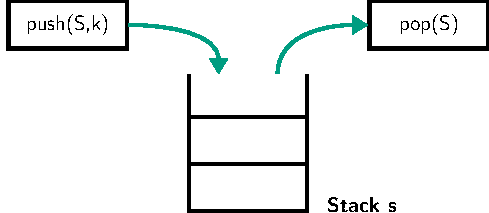
\includegraphics[width=6cm]{pictures/LIFO/lifo}
                    \end{itemize}
          \end{itemize}

    \item \fatsf{}{Beispiel Bitcoin}
    \item[] 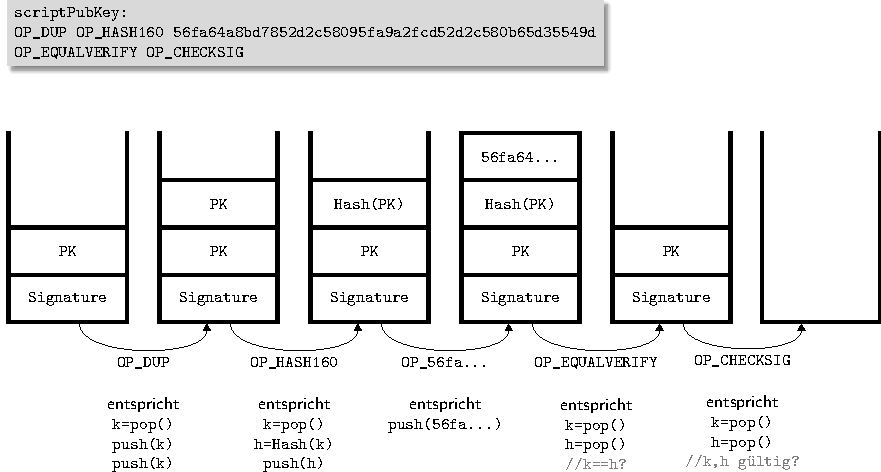
\includegraphics[width=15cm]{pictures/bitcoin_stack_example/bitcoin_stack_example}
          \clearpage
    \item \fatsf{Stacks als Array}
          \begin{itemize}
              \item[] 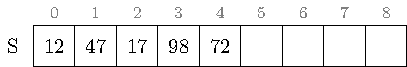
\includegraphics[]{pictures/staack_als_array/stack_als_array}
              \item \texttt{s.top} zeigt immer auf oberstes Element
              \item \texttt{pop()} führt dazu, dass \texttt{s.Top} sich eins nach links bewegt
              \item \texttt{push(k)} führt dazu, dass \texttt{s.Top} sich eins nach rechts bewegt
          \end{itemize}

    \item \fatsf{Stacks als Array - Methoden, falls maximale Größe bekannt}\\
          \begin{minipage}[t]{.4\textwidth}
              \begin{ccode}[autogobble]{title=new(S)}
                  S.A[]=ALLOCATE(MAX);
                  S.TOP=-1;
              \end{ccode}
          \end{minipage}
          \begin{minipage}[t]{.4\textwidth}
              \begin{ccode}[autogobble]{title=isEmpty(S)}
                  IF S.top<0 THEN
                    return true;
                  ELSE
                    return false;
              \end{ccode}
          \end{minipage}
          \\
          \begin{minipage}[t]{.4\textwidth}
              \begin{ccode}[autogobble]{title=pop(S)}
                  IF isEmpty(S) THEN
                    error "underflow";
                  ELSE
                    s.top=s.top-1;
                    return S.A[S.top+1];
              \end{ccode}
          \end{minipage}
          \begin{minipage}[t]{.4\textwidth}
              \begin{ccode}[autogobble]{title=push(S)}
                  IF S.top==MAX-1 THEN
                    error "overflow";
                  ELSE
                    S.top=S.top+1;
                    S.A[S.top]=k;
              \end{ccode}
          \end{minipage}
          %\item[] 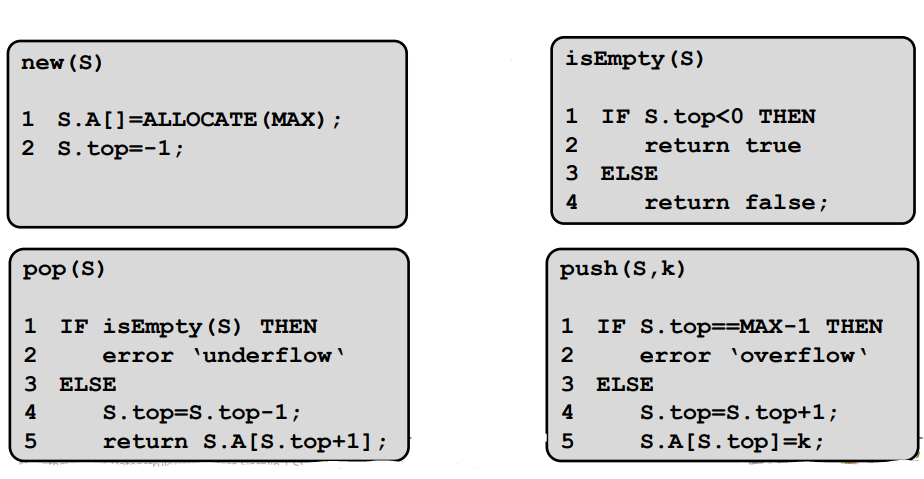
\includegraphics[width=12cm]{pictures/arrayMethods1}

    \item \fatsf{Stacks mit variabler Größe - Einfach}
          \begin{itemize}
              \item Falls \texttt{push(k)} bei vollem Array $\Rightarrow$ Vergößerung des Arrays
              \item Erzeugen eines neuen Arrays mit Länge + 1 und Umkopieren aller Elemente
              \item Durchschnittlich $\Omega(n)$ Kopierschritte pro \texttt{push}-Befehl
          \end{itemize}
          \clearpage
    \item \fatsf{Stacks mit variabler Größe - Verbesserung}
          \begin{itemize}
              \item Idee:
                    \begin{itemize}
                        \item Wenn Grenze erreicht, Verdopplung des Speichers und Kopieren der Elemente
                        \item Falls weniger als ein Viertel belegt, schrumpfe das Array wieder
                    \end{itemize}
              \item Methoden:
              \item[] \texttt{RESIZE(A,m)} reserviert neuen Speicher der Grö\ss e \texttt{m} und kopiert \texttt{A} um\\
                    \begin{minipage}[t]{.5\textwidth}
                        \begin{ccode}[autogobble]{title=new(S)}
                            S.A[]=ALLOCATE(1);
                            S.TOP=-1;
                            S.memsize=1;
                        \end{ccode}
                    \end{minipage}
                    \begin{minipage}[t]{.4\textwidth}
                        \begin{ccode}[autogobble]{title=isEmpty(S)}
                            IF S.top<0 THEN
                                return true;
                            ELSE
                                return false;
                        \end{ccode}
                    \end{minipage}
                    \\
                    \begin{minipage}[t]{.5\textwidth}
                        \begin{ccode}[autogobble]{title=pop(S)}
                            IF isEmpty(S) THEN
                                error "underflow";
                            ELSE
                                S.top=S.top-1;
                                IF 4*(S.top+1)==S.memsize THEN
                                    S.mensize=s.memsize/2;
                                    RESIZE(S.A,S.memsize);
                                return S.A[S.top+1];
                        \end{ccode}
                    \end{minipage}
                    \begin{minipage}[t]{.4\textwidth}
                        \begin{ccode}[autogobble]{title=push(S)}
                            S.top=S.top+1;
                            S.A[S.top]=k;
                            IF S.top+1>=S.memsize THEN
                                S.memsize=2*S.memsize;
                                RESIZE(S.A,S.memsize);
                        \end{ccode}
                    \end{minipage}
                    %\item[] 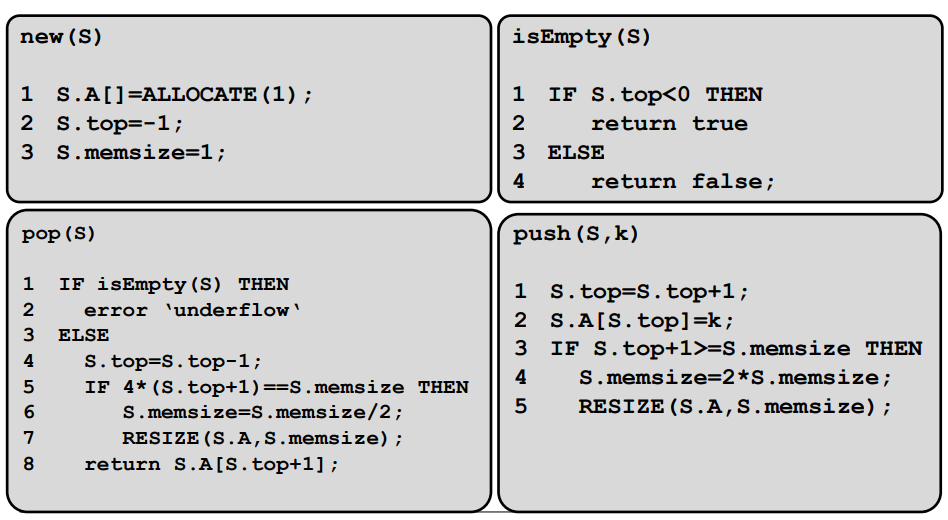
\includegraphics[width=12cm]{pictures/stacksArray2.PNG}

              \item Im Durchschnitt für jeder der mindestens \texttt{n} Befehle $\Theta(1)$ Umkopierschritte

          \end{itemize}
\end{itemize}

\pagebreak
\subsection{Verkettete Listen}\label{Verkettete Listen}
\begin{itemize}
    \item \fatsf{Aufbau}
          \begin{itemize}
              \item[] 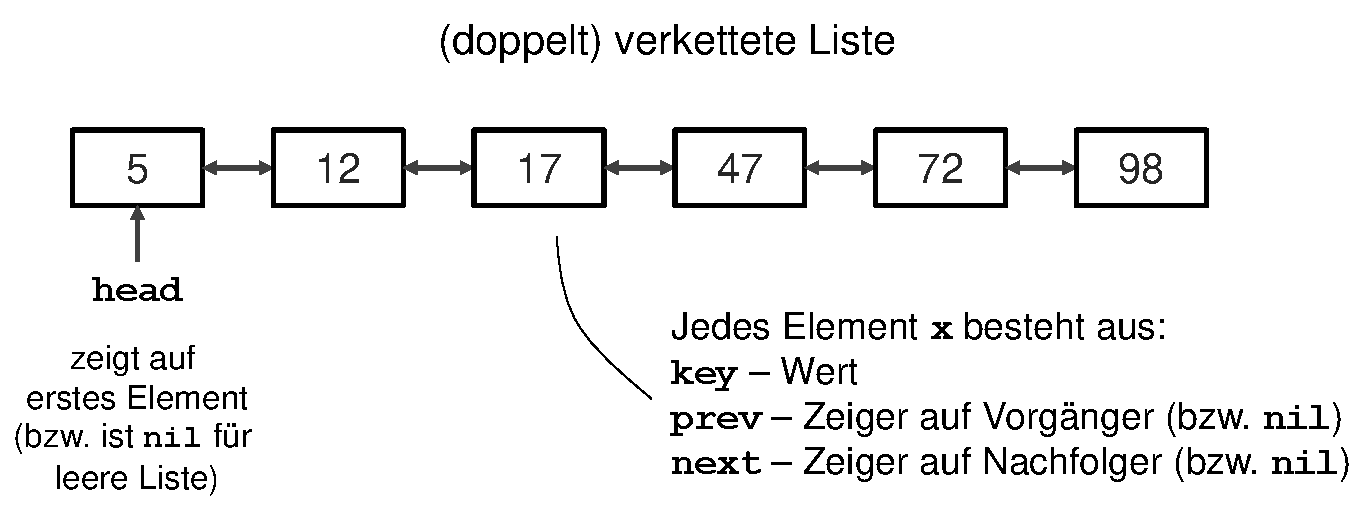
\includegraphics[width=12cm]{pictures/linkedList1.pdf}
          \end{itemize}

    \item \fatsf{Verkettete Listen durch Arrays}
          \begin{itemize}
              \item[] Entspricht doppelter Verkettung zwischen 45 und 12
              \item[] 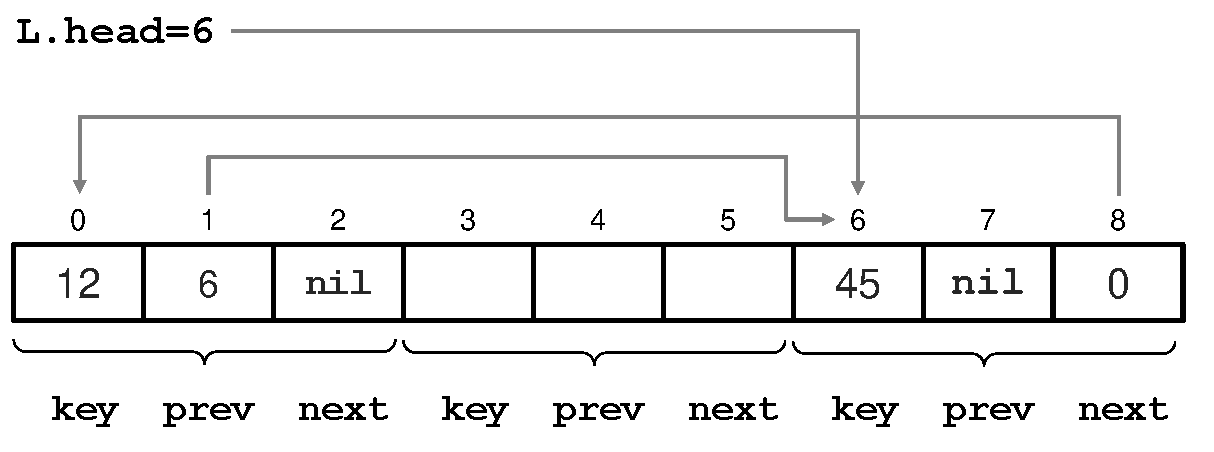
\includegraphics[width=12cm]{pictures/linkedList2.pdf}
          \end{itemize}

    \item \fatsf{Elementare Operationen auf Listen}
          \begin{itemize}
              \item \textit{Suche nach Element}
                    \begin{itemize}
                        \item Laufzeit beträgt im Worst Case $\Theta(n)$
                        \item[] $\Rightarrow$ Keine Überprüfung, ob Wert bereits in Liste, sonst $\Theta(n)$
                        \item Code:
                        \item[]
                              \begin{ccode}[autogobble]{title={search(L,k) // Returns pointer to k in L (or nil)}}
                                  current = L.head;
                                  WHILE current != nil AND current.key != k DO
                                    current = current.next;
                                  return current;
                              \end{ccode}
                        \item[] 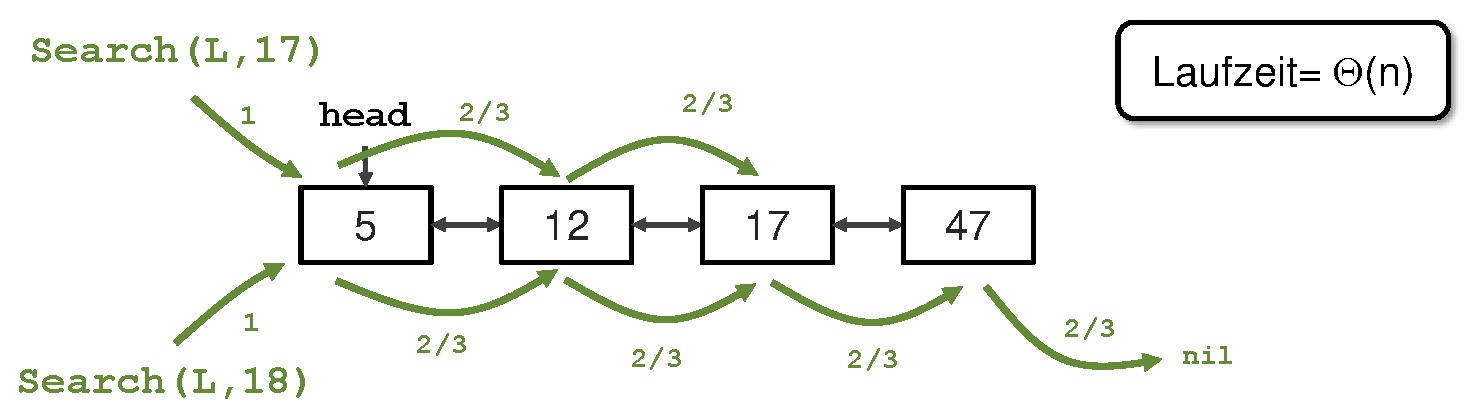
\includegraphics[width=12cm]{pictures/verketteteListenSuche.pdf}
                    \end{itemize}

                    \clearpage
              \item \textit{Einfügen eines Elements am Kopf der Liste}
                    \begin{itemize}
                        \item Laufzeit beträgt $\Theta(1)$, da Einfügen am Kopf
                        \item Code:
                        \item[]
                              \begin{ccode}[autogobble]{title={insert(L,x)}}
                                  insert(L,x)
                                  x.next = l.head;
                                  x.prev = nil;
                                  IF L.head != nil THEN
                                    L.head.prev = x;
                                  L.head = x;
                              \end{ccode}
                    \end{itemize}

              \item \textit{Löschen eines Elements aus Liste}
                    \begin{itemize}
                        \item Laufzeit beträgt $\Theta(1)$, da hier Pointer auf Objekt gegeben
                        \item[] Löschen eines Wertes $k$ mithilfe von Suche beträgt $\Omega(n)$
                        \item Code:
                        \item[]
                              \begin{ccode}[autogobble]{title={delete (L,x)}}
                                  IF x.prev != nil THEN
                                    x.prev.next = x.next
                                  ELSE
                                    L.head = x.next;
                                  IF x.next != nil THEN
                                    x.next.prev = x.prev;
                              \end{ccode}
                    \end{itemize}
          \end{itemize}

    \item \fatsf{Vereinfachung per Wächter/Sentinels}
          \begin{itemize}
              \item Ziel ist die Eliminierung der Spezialfälle für Listenanfang/-ende
              \item[] 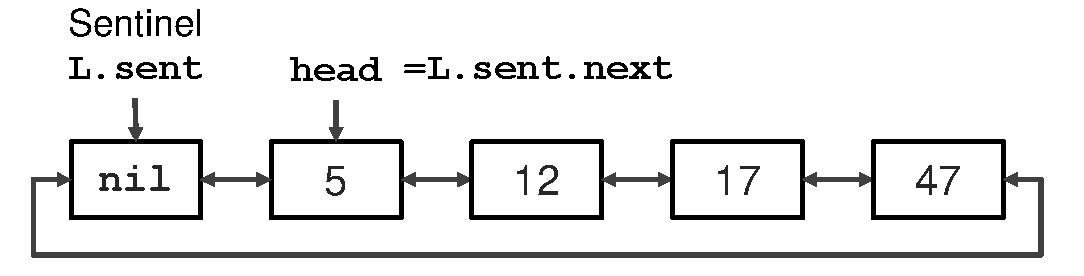
\includegraphics[width=12cm]{pictures/linkedListSentinel.pdf}
              \item Löschen mit Sentinels:
              \item[]
                    \begin{ccode}[autogobble]{title={deleteSent(L,x)}}
                        x.prev.next = x.next;
                        x.next.prev = x.prev;
                    \end{ccode}
          \end{itemize}
\end{itemize}
\clearpage
\subsection{Queues}\label{Queues}
\begin{itemize}
    \item \textbf{Abstrakter Datentyp Queue}
          \begin{itemize}
              \item \texttt{new Q()}
                    \begin{itemize}
                        \item Erzeuge neue (leere) Queue
                    \end{itemize}

              \item \texttt{q.isEmpty()}
                    \begin{itemize}
                        \item Gibt an, ob Queue \texttt{q} leer ist
                    \end{itemize}

              \item \texttt{q.dequeue()}
                    \begin{itemize}
                        \item Gibt vorderstes Element aus \texttt{q} zurück und löscht es auf Queue
                        \item Fehlermeldung, falls Queue leer ist
                    \end{itemize}

              \item \texttt{q.enqueue(k)}
                    \begin{itemize}
                        \item Schreibt \texttt{k} als neues hinterstes Element auf \texttt{q}
                        \item Fehlermeldung, falls Queue voll ist
                    \end{itemize}

              \item Abstrakter Aufbau:
                    \begin{itemize}
                        \item \fatsf{FIFO}-Prinzip / First in, First out
                        \item[] 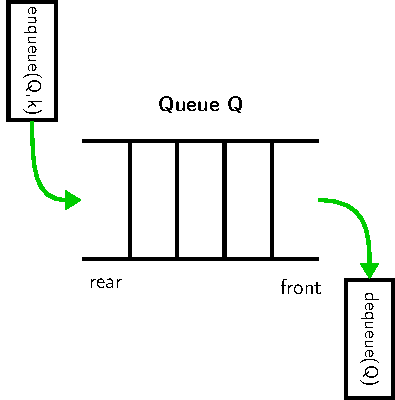
\includegraphics[width=8cm]{pictures/FIFO/FIFO}
                    \end{itemize}
          \end{itemize}

          \pagebreak

    \item \fatsf{Queues als (virtuelles) zyklisches Array}
          \begin{itemize}
              \item[] Bekannt: Maximale Elemente gleichzeitig in Queue
              \item[] 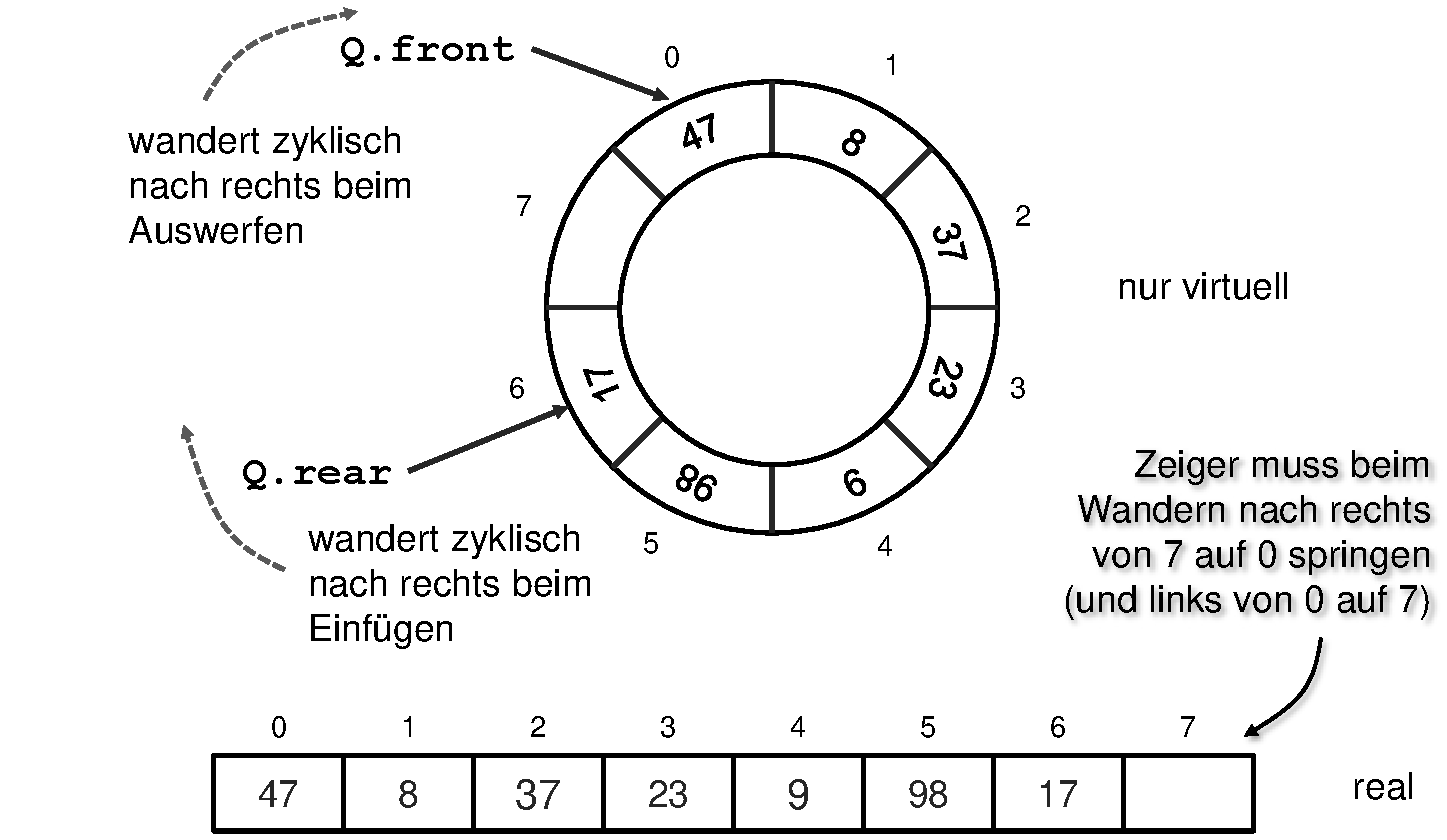
\includegraphics[width=12cm]{pictures/queueZyklisch.pdf}
              \item[]
              \item Problem, falls \texttt{Q.rear} und \texttt{Q.front} auf selbes Element zeigen
                    \begin{itemize}
                        \item Speichere Information, ob Schlange leer oder voll, in boolean \texttt{empty}
                        \item Alternativ: Reserviere ein Element des Arrays als Abstandshalter
                    \end{itemize}

              \item Methoden für zyklisches Array\\
                    \begin{minipage}[t]{.45\textwidth}
                        \begin{ccode}[autogobble]{title={new(Q)}}
                            Q.A[]=ALLOCATE(MAX);
                            Q.front=0;
                            Q.rear=0;
                            Q.empty=true;
                        \end{ccode}
                    \end{minipage}
                    \begin{minipage}[t]{.45\textwidth}
                        \begin{ccode}[autogobble]{title={isEmpty(Q)}}
                            return Q.empty;
                        \end{ccode}
                    \end{minipage}
                    \\
                    \begin{minipage}[t]{.45\textwidth}
                        \begin{ccode}[autogobble]{title={dequeue(Q)}}
                            IF isEmpty(Q) THEN
                                error "underflow";
                            ELSE
                                Q.front=Q.front+1 mod MAX;
                                IF Q.front==Q.rear THEN
                                    Q.empty=true;
                                return Q.A[Q.front-1 mod MAX];
                        \end{ccode}
                    \end{minipage}
                    \begin{minipage}[t]{.45\textwidth}
                        \begin{ccode}[autogobble]{title={enqueue(Q,k)}}
                            IF Q.rear==Q.front AND !Q.isEmpty
                            THEN error "overflow";
                            ELSE
                                Q.A[Q.rear]=k;
                                Q.rear=Q.rear+1 mod MAX;
                                Q.empty=false;
                        \end{ccode}
                    \end{minipage}
                    %\item[] 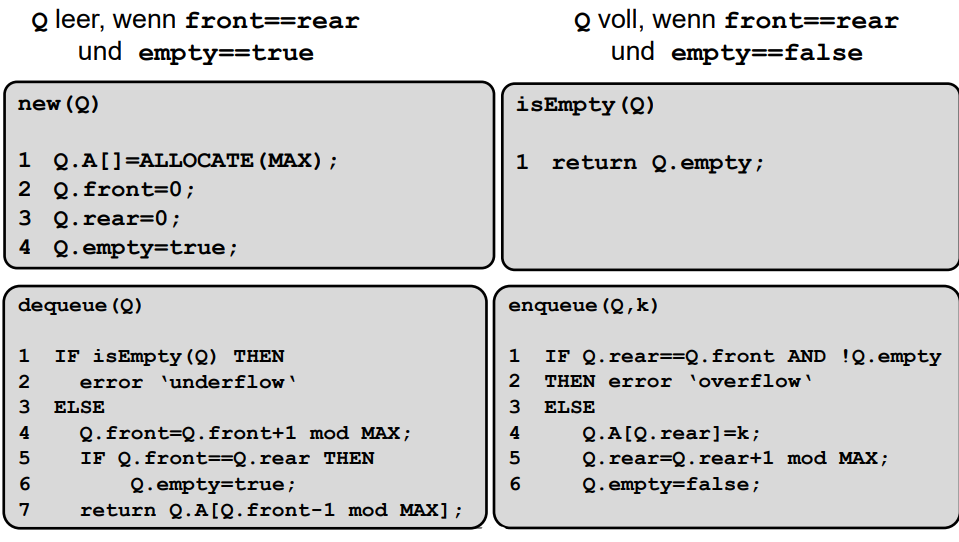
\includegraphics[width=12cm]{pictures/queueZyklischM.PNG}
          \end{itemize}

          \pagebreak

    \item \textbf{Queues durch einfach verkettete Listen}
          \begin{itemize}
              \item[] 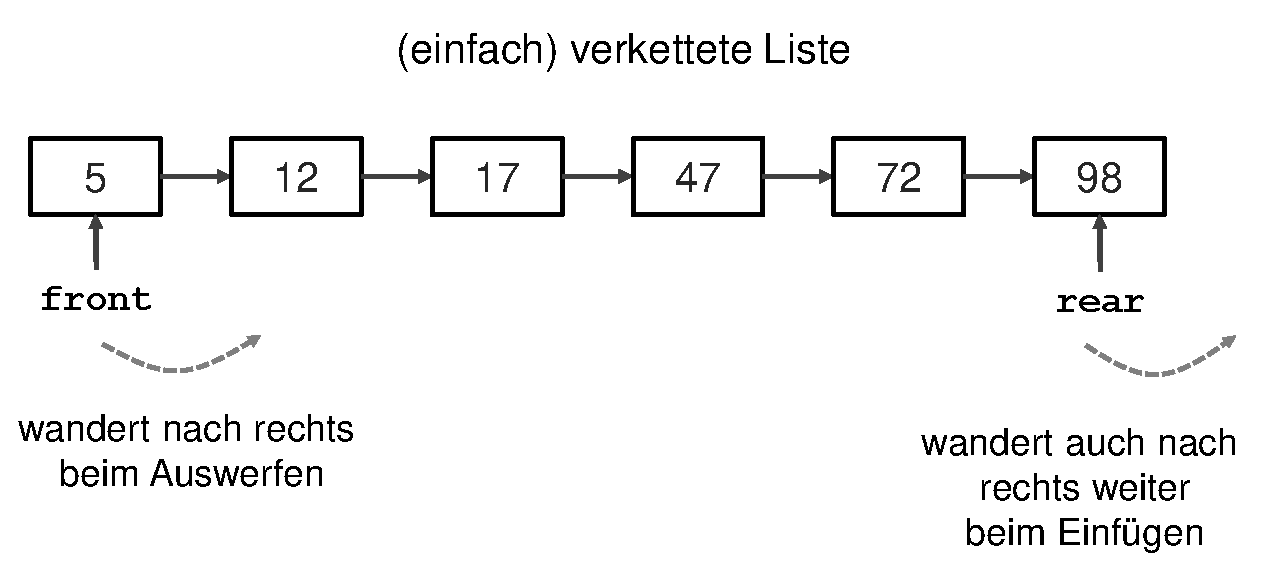
\includegraphics[width=12cm]{pictures/queuesListe1.pdf}
              \item[] Methoden:
              \item[] %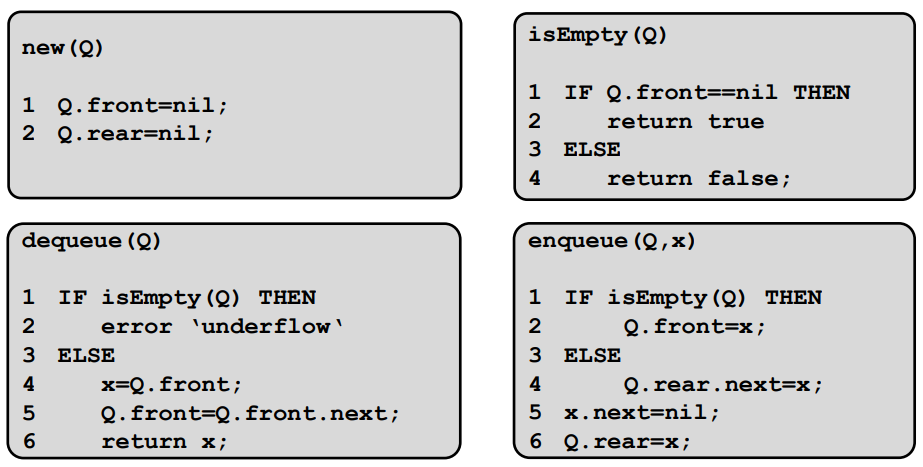
\includegraphics[width=12cm]{pictures/queuesListe2.PNG} 
                    \begin{minipage}[t]{.4\textwidth}
                        \begin{ccode}[autogobble]{title={new(Q)}}
                            Q.front=nil;
                            Q.rear=nil;
                        \end{ccode}
                    \end{minipage}
                    \begin{minipage}[t]{.4\textwidth}
                        \begin{ccode}[autogobble]{title={isEmpty(Q)}}
                            IF Q.front==nil THEN
                                return true;
                            ELSE
                                return false;
                        \end{ccode}
                    \end{minipage}
                    \\
                    \begin{minipage}[t]{.4\textwidth}
                        \begin{ccode}[autogobble]{title={dequeue(Q)}}
                            IF isEmpty(Q) THEN
                                error "underflow";
                            ELSE
                                x=Q.front;
                                Q.front=Q.front.next;
                                return x;
                        \end{ccode}
                    \end{minipage}
                    \begin{minipage}[t]{.4\textwidth}
                        \begin{ccode}[autogobble]{title={enqueue(Q,k)}}
                            IF isEmpty(Q) THEN
                                Q.front=x;
                            ELSE
                                Q.rear.next=x;
                            x.next=nil;
                            Q.rear=x;
                        \end{ccode}
                    \end{minipage}
          \end{itemize}

    \item \fatsf{Laufzeit}
          \begin{itemize}
              \item Enqueue: $\Theta(1)$
              \item Dequeue: $\Theta(1)$
          \end{itemize}
\end{itemize}

\pagebreak
\subsection{Binäre Bäume}\label{Binaere Baeume}
\begin{itemize}
    \item \fatsf{Bäume durch verkettete Listen}
          \begin{itemize}
              \item[] \includegraphics[width=12cm]{pictures/binäreBaumeListe.PNG}
              \item[] Bäume sind \string"azyklisch\string" (Keine "rückführende Spur")
          \end{itemize}

    \item \fatsf{Darstellung als (ungerichteter) Graph}
          \begin{itemize}
              \item[]
                    \begin{minipage}[t]{0.45\textwidth}
                        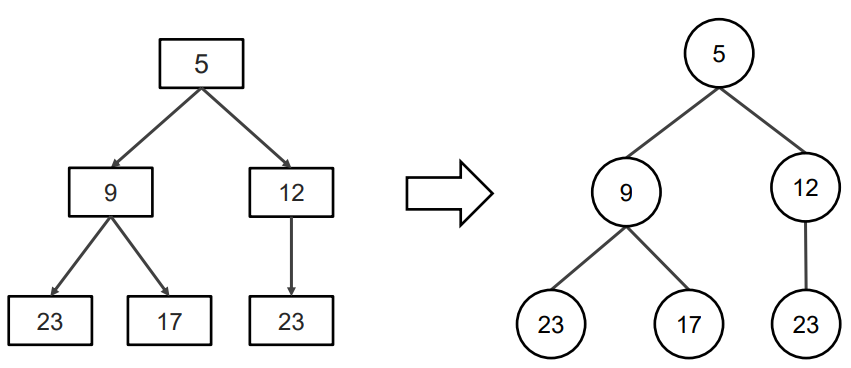
\includegraphics[width=7cm]{pictures/baumGraph1.PNG}
                    \end{minipage}
                    \begin{minipage}[t]{0.45\textwidth}
                        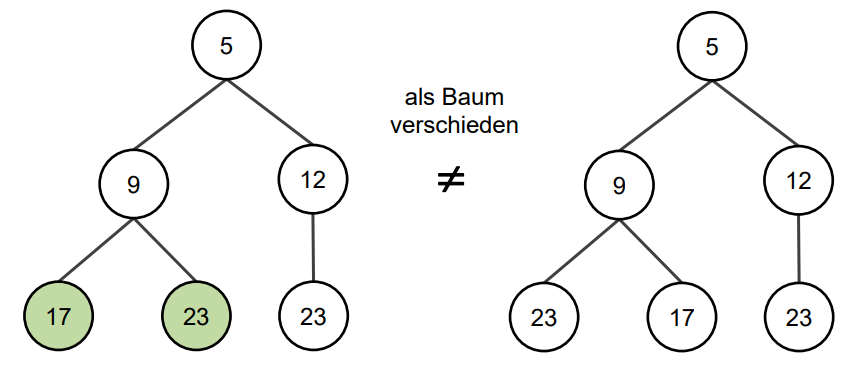
\includegraphics[width=7cm]{pictures/baumGraph2.PNG}
                    \end{minipage}
          \end{itemize}

    \item \fatsf{Allgemeine Begrifflichkeiten}
          \begin{itemize}
              \item[]
                    \begin{minipage}[t]{0.45\textwidth}
                        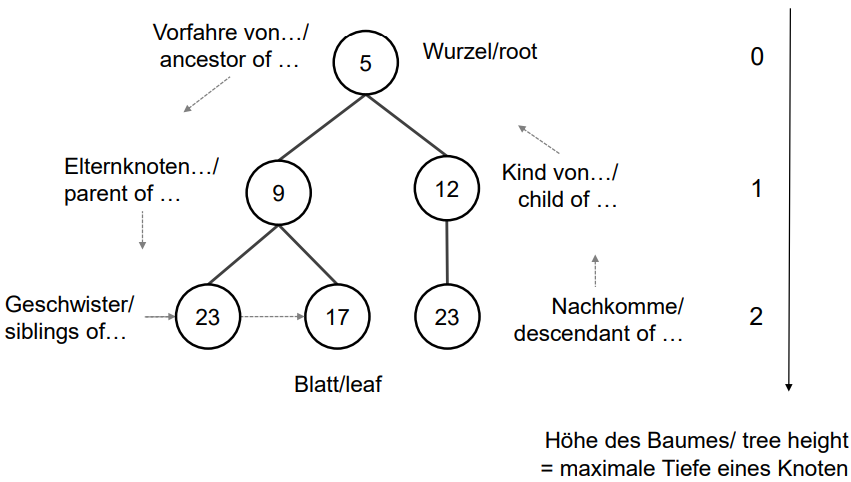
\includegraphics[width=8cm]{pictures/baumBegriffe1.PNG}
                    \end{minipage}
                    \begin{minipage}[t]{0.45\textwidth}
                        \vspace{-3.5cm}
                        \begin{itemize}
                            \item Blatt: Knoten ohne Nachfolger
                            \item Nachkomme von x: \\
                                  Erreichbar durch Pfad ausgehend von x
                        \end{itemize}
                    \end{minipage}
          \end{itemize}
          \clearpage
    \item \fatsf{Begrifflichkeiten Binärbaum}
          \begin{itemize}
              \item[]
                    \begin{minipage}[t]{0.45\textwidth}
                        \includegraphics[width=8cm]{pictures/binärbaumBegriffe}
                    \end{minipage}
                    \begin{minipage}[t]{0.45\textwidth}
                        \vspace{-4.5cm}
                        \begin{itemize}
                            \item Jeder Knoten hat maximal zwei Kinder \\
                                  \texttt{left=child[0]} und \texttt{right=child[1]}
                            \item Ausgangsgrad jedes Knoten ist $\leq 2$
                            \item Höhe leerer Baum per Konvention $-1$
                            \item Hohe (nicht-leerer) Baum: \\
                                  max\{Höhe aller Teilbäume der Wurzel\} + 1
                            \item Halbblatt: Knoten mit nur einem Kind
                        \end{itemize}
                    \end{minipage}
          \end{itemize}


    \item \fatsf{Traversieren von Bäumen}
          \begin{itemize}
              \item Darstellung eines Baumes mithilfe einer Liste der Werte aller Knoten
              \item Laufzeit bei $n$ Knoten: $T(n) = O(n)$
              \item Nutzung der Preorder für das Kopieren von Bäumen
                    \begin{enumerate}
                        \item Preorder betrachtet Knoten und legt Kopie an
                        \item Preorder geht dann in Teilbäume und kopiert diese
                    \end{enumerate}
              \item Nutzung der Postorder für das Löschen von Bäumen
                    \begin{enumerate}
                        \item Postorder geht zuerst in Teilbäume und löscht diese
                        \item Betrachten des Knoten erst danach und dann Löschung dieses
                    \end{enumerate}
              \item[]
              \item[]
                    \begin{minipage}[t]{0.4\textwidth}
                        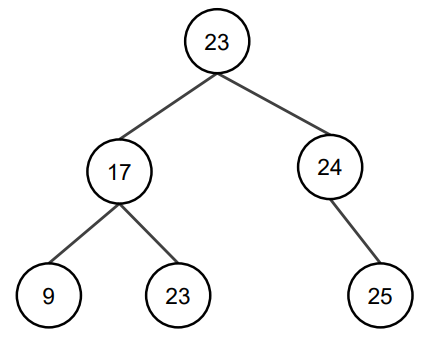
\includegraphics[width=6cm]{pictures/inorder1}
                    \end{minipage}
                    \begin{minipage}[t]{0.5\textwidth}
                        \vspace{-4.75cm}
                        \begin{itemize}
                            \item[] 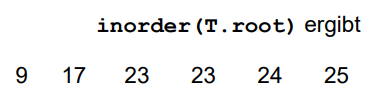
\includegraphics[width=6cm]{pictures/inorder2}
                            \item[] 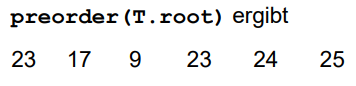
\includegraphics[width=6cm]{pictures/preorder1}
                            \item[] 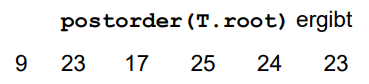
\includegraphics[width=6cm]{pictures/postorder1}
                        \end{itemize}
                    \end{minipage}
              \item[]
              \item[] \textbf{Code:} \\
                    \begin{minipage}[t]{0.29\textwidth}
                        \begin{ccode}[autogobble]{title={inorder(x)}}
                            IF x != nil THEN
                                inorder(x.left);
                                print x.key;
                                inorder(x.right);
                        \end{ccode}
                    \end{minipage}
                    \begin{minipage}[t]{0.3\textwidth}
                        \begin{ccode}[autogobble]{title={preorder(x)}}
                            IF x != nil THEN
                                print x.key;
                                preorder(x.left);
                                preorder(x.right);
                        \end{ccode}
                    \end{minipage}
                    \begin{minipage}[t]{0.31\textwidth}
                        \begin{ccode}[autogobble]{title={postorder(x)}}
                            IF x != nil THEN
                                postorder(x.left);
                                postorder(x.right);
                                print x.key;
                        \end{ccode}
                    \end{minipage}
          \end{itemize}
          \clearpage
    \item \fatsf{Eindeutige Bestimmbarkeit von Bäumen}
          \begin{itemize}
              \item Nur In-,Pre-,Postorder reichen nicht zur eindeutigen Bestimmbarkeit von Bäumen
              \item[] $\Rightarrow$ Preorder/Postorder $+$ Inorder $+$ eindeutige Werte sind notwendig
              \item[] 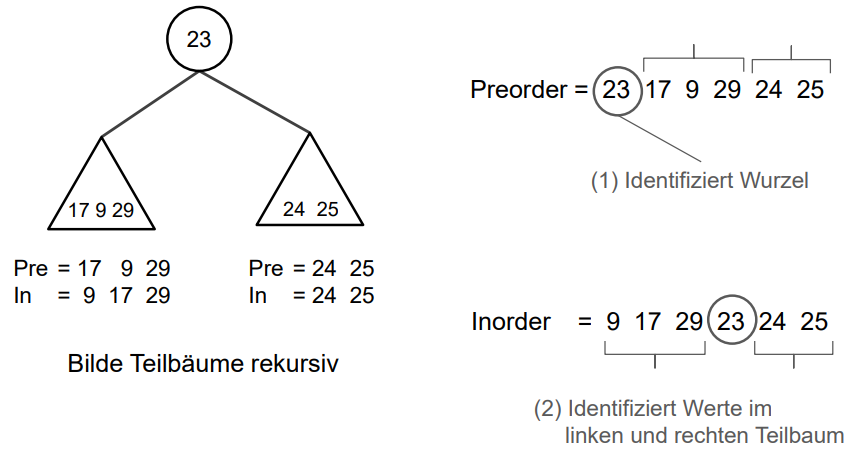
\includegraphics[width=12cm]{pictures/bestimmbarkeitBaum.PNG}
          \end{itemize}


    \item \fatsf{Abstrakter Datentyp Baum}
          \begin{itemize}
              \item \textit{Abstrakter Aufbau:}
                    \begin{itemize}
                        \item \texttt{new T()}
                              \begin{itemize}
                                  \item Erzeugt neuen Baum namens \texttt{t}
                              \end{itemize}

                        \item \texttt{t.search(k)}
                              \begin{itemize}
                                  \item Gibt Element \texttt{x} in Baum \texttt{t} mit \texttt{x.key == k} zurück
                              \end{itemize}

                        \item \texttt{t.insert(k)}
                              \begin{itemize}
                                  \item Fügt Element \texttt{x} in Baum \texttt{t} hinzu
                              \end{itemize}

                        \item \texttt{t.delete(x)}
                              \begin{itemize}
                                  \item Löscht \texttt{x} aus Baum \texttt{t}
                              \end{itemize}
                    \end{itemize}

              \item \textit{Suche nach Elementen:}
                    \begin{itemize}
                        \item Laufzeit = $\Theta(n)$ (Jeder Knoten maximal einmal, jeder Knoten im schlechtesten Fall)
                        \item Starte mit \texttt{search(T.root,k)}
                        \item Code:
                        \item[]
                              \begin{ccode}[autogobble]{title={search(x,k)}}
                                  IF x == nil THEN return nil;
                                  IF x.key == k THEN return x;
                                  y = search(x.left,k);
                                  IF y != nil THEN return y;
                                  return search(x.right,k);
                              \end{ccode}
                    \end{itemize}
                    \clearpage
              \item \textit{Einfügen von Elementen:}
                    \begin{itemize}
                        \item Laufzeit = $\Theta(1)$
                        \item Hier wird als Wurzel eingefügt (Achtung: Erzeugt linkslastigen Baum)
                        \item Code:
                        \item[]
                              \begin{ccode}[autogobble]{title={insert(T,x) // x.parent == x.left == x.right == nil;}}
                                  IF T.root != nil THEN
                                    T.root.parent = x;
                                    x.left = T.root;
                                  T.root = x;
                              \end{ccode}
                    \end{itemize}

              \item \textit{Löschen von Elementen:}
                    \begin{itemize}
                        \item Laufzeit = $\Theta(h)$ (Höhe des Baumes, $h=n$ möglich)
                        \item Hier: Ersetze $x$ durch Halbblatt ganz rechts
                        \item[] \includegraphics[width=12cm]{pictures/löschenBaum.PNG}
                              \pagebreak
                        \item \texttt{Connect}-Algorithmus:
                        \item[]
                              \begin{minipage}[t]{0.35\textwidth}
                                  \includegraphics[width=5cm]{pictures/löschenBaumConnect.PNG}
                              \end{minipage}
                              \begin{minipage}[t]{0.45\textwidth}
                                  \vspace{-7cm}
                                  \begin{itemize}
                                      \item Laufzeit = $\Theta(1)$
                                      \item[]
                                            \begin{ccode}[autogobble]{title={connect(T,y,w) // Connects w to y.parent}}
                                                v = y.parent;
                                                IF y != T.root THEN
                                                    IF y == v.right THEN
                                                        v.right = w;
                                                    ELSE
                                                        v.left = w;
                                                ELSE
                                                    T.root = w;
                                                IF w != nil THEN
                                                    w.parent = v;
                                            \end{ccode}
                                  \end{itemize}
                              \end{minipage}

                        \item \texttt{Delete}-Algorithmus:
                        \item[]
                              \begin{minipage}{0.4\textwidth}
                                  \includegraphics[width=6cm]{pictures/löschenBaumDelete.PNG}
                              \end{minipage}
                              \begin{minipage}{0.45\textwidth}
                                  \begin{itemize}
                                      \item[]
                                            \begin{ccode}[autogobble]{title={delete(T,x) // assumes x in T}}
                                                y = T.root;
                                                WHILE y.right != nil DO
                                                    y = y.right;
                                                connect(T,y,y.left);
                                                IF x != y THEN
                                                    y.left = x.left;
                                                    IF x.left != nil THEN
                                                        x.left.parent = y;
                                                    y.right = x.right;
                                                    IF x.right != nil THEN
                                                        x.right.parent = y;
                                                    connect(T,x,y);
                                            \end{ccode}
                                  \end{itemize}
                              \end{minipage}
                    \end{itemize}
          \end{itemize}
\end{itemize}

\pagebreak
\subsection{Binäre Suchbäume}\label{Binaere Suchbaeume}
\begin{itemize}
    \item \fatsf{Definition}
          \begin{itemize}
              \item Totale Ordnung auf den Werten
              \item Für alle Knoten $z$ gilt:
              \item[] Wenn $x$ Knoten im linken Teilbaum von $z$, dann \texttt{x.key $\leq$ z.key}
              \item[] Wenn $y$ Knoten im rechten Teilbaum von $z$, dann \texttt{y.key $\geq$ z.key}
              \item Preorder/Postorder + eindeutige Werte $\Rightarrow$ Eindeutige Identifizierung
          \end{itemize}

    \item \fatsf{Suchen im Binären Suchbaum}
          \begin{itemize}
              \item[]
                    \begin{minipage}{0.4\textwidth}
                        \includegraphics[width=8cm]{pictures/binärerSuchbaumSuche.PNG}
                    \end{minipage}
                    \begin{minipage}{0.5\textwidth}
                        \begin{itemize}
                            \item Laufzeit $= O(h)$ (Höhe)
                            \item Code:
                            \item[]
                                  \begin{ccode}[autogobble]{title={search(x,k) // 1. Aufruf x = root}}
                                      IF x == nil OR x.key == k THEN
                                        return x;
                                      IF x.key > k THEN
                                        return search(x.left,k);
                                      ELSE
                                        return search(x.right,k);
                                  \end{ccode}
                            \item Iterativer Code:
                            \item[]
                                  \begin{ccode}[autogobble]{title={iterative-search(x,k)}}
                                      WHILE x != nil AND x.key != k DO
                                        IF x.key > k THEN
                                            x = x.left;
                                        ELSE
                                            x = x.right;
                                      return x;
                                  \end{ccode}
                        \end{itemize}
                    \end{minipage}
          \end{itemize}
          \clearpage
    \item \fatsf{Einfügen im Binary Search Tree}
          \begin{itemize}
              \item[]
                    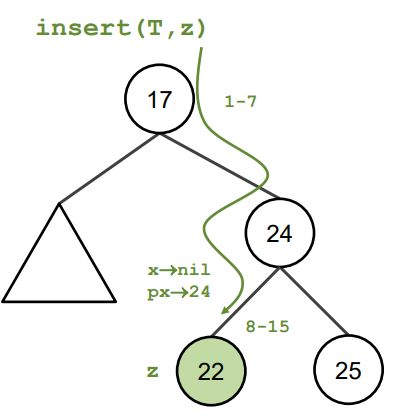
\includegraphics[width=8cm]{pictures/binärerSuchbaumEinfügen.PNG}
                    \begin{itemize}
                        \item Laufzeit = $O(h)$
                        \item Aufwendiger, da Ordnung erhalten werden muss
                        \item Code:
                        \item[]\label{BST-Insert}
                              \begin{ccode}[autogobble]{title={insert (T,z) // z.left == z.right == nil;}}
                                  x = T.root;
                                  px = nil;
                                  WHILE x != nil DO
                                    px = x;
                                    IF x.key > z.key THEN
                                        x = x.left;
                                    ELSE
                                        x = x.right;
                                  z.parent = px;
                                  IF px == nil THEN
                                    T.root = z;
                                  ELSE
                                    IF px.key > z.key THEN
                                        px.left = z;
                                    ELSE
                                        px.right = z;
                              \end{ccode}
                    \end{itemize}
          \end{itemize}

          \pagebreak

    \item \fatsf{Löschen im BST}
          \begin{itemize}
              \item \textit{Verschiedene Fälle:}
                    \begin{itemize}
                        \item[] 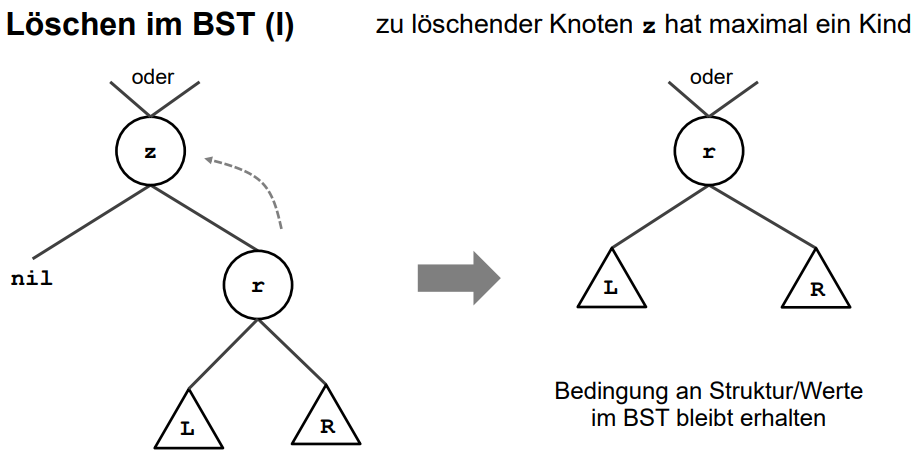
\includegraphics[width=9cm]{pictures/binärerSuchbaumLöschen1.PNG}
                        \item[] 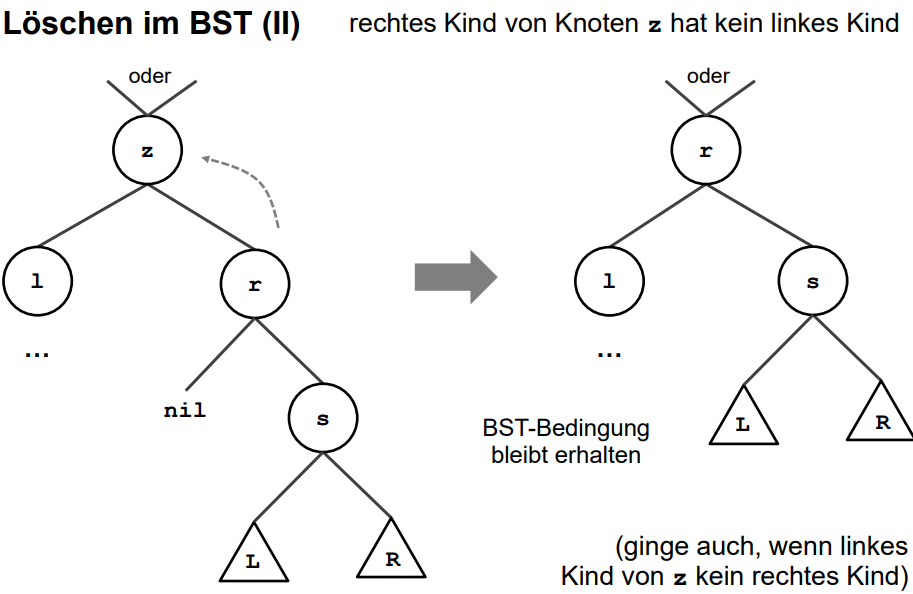
\includegraphics[width=9cm]{pictures/binärerSuchbaumLöschen2.PNG}
                        \item[] 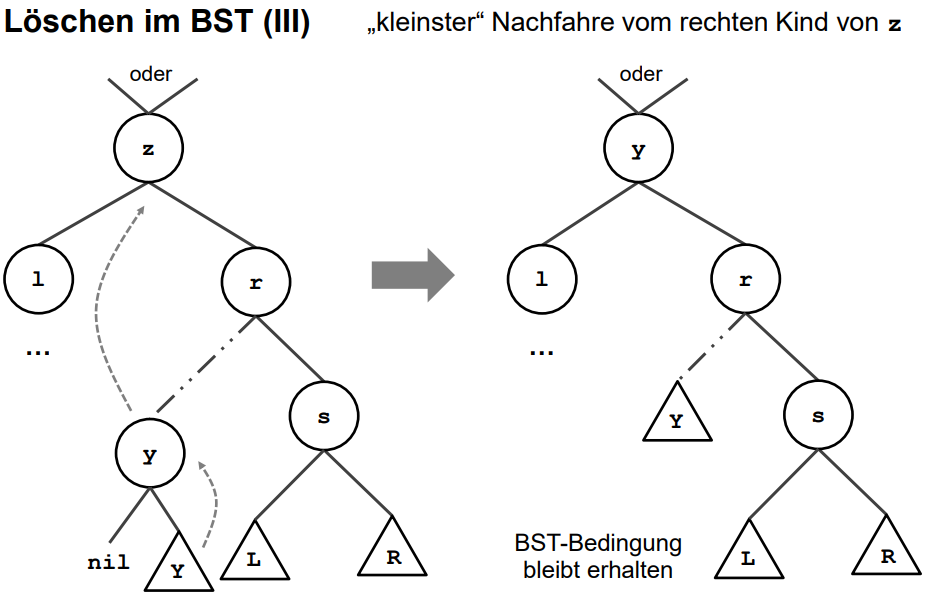
\includegraphics[width=9cm]{pictures/binärerSuchbaumLöschen3.PNG}
                    \end{itemize}
                    \clearpage
              \item \textit{Code}
              \item[]
                        \begin{ccode}[autogobble]{title={transplant(T,u,v) // Hängt Teilbaum v an Parent von u}}
                            IF u.parent == nil THEN
                                T.root = v;
                            ELSE
                                IF u == u.parent.left THEN
                                    u.parent.left = v;
                                ELSE
                                    u.parent.right = v;
                            IF v != nil THEN
                                v.parent = u.parent;
                        \end{ccode}
                        \begin{ccode}[autogobble]{title={delete(T,z)}}
                            IF z.left == nil THEN
                                transplant(T,z,z.left)
                            ELSE
                                IF z.right == nil THEN
                                    transplant(T,z,z,left)
                                ELSE
                                    y = z.right;
                                    WHILE y.left != nil DO y = y.left;
                                    IF y.parent != z THEN
                                        transplant(T,y,y.right)
                                        y.right = z.right;
                                        y.right.parent = y;
                                    transplant(T,z,y)
                                    y.left = z.left;
                                    y.left.parent = y;
                        \end{ccode}
              \item Laufzeit = $O(h)$
              \item Laufzeit ist damit besser, wenn viele Suchoperationen und $h$ klein relativ zu $n$
          \end{itemize}
\clearpage
    \item \fatsf{Höhe eines BST}
          \begin{itemize}
              \item \textit{Best Case:}
                    \begin{itemize}
                        \item Vollständiger Baum (Alle Blätter gleiche Tiefe)
                        \item $h = O(log_2 n)$
                        \item Laufzeit = $O(log_2 n)$
                    \end{itemize}
              \item \textit{Worst Case:}
                    \begin{itemize}
                        \item Degenerierter Baum (lineare Liste)
                        \item $h = n - 1$
                        \item Laufzeit = $\Theta(n)$
                    \end{itemize}
              \item \textit{Durchschnittliche Höhe:}
                    \begin{itemize}
                        \item Erwartete Höhe: $\Theta(log_2 n)$
                    \end{itemize}
          \end{itemize}
    \item \fatsf{Suchbäume als Suchindex}
          \begin{itemize}
              \item Knoten speichert nur Primärschlüssel und Zeiger auf Daten
              \item Zusätzliche Indizes möglich, kosten aber Speicherplatzbedarf
              \item[] 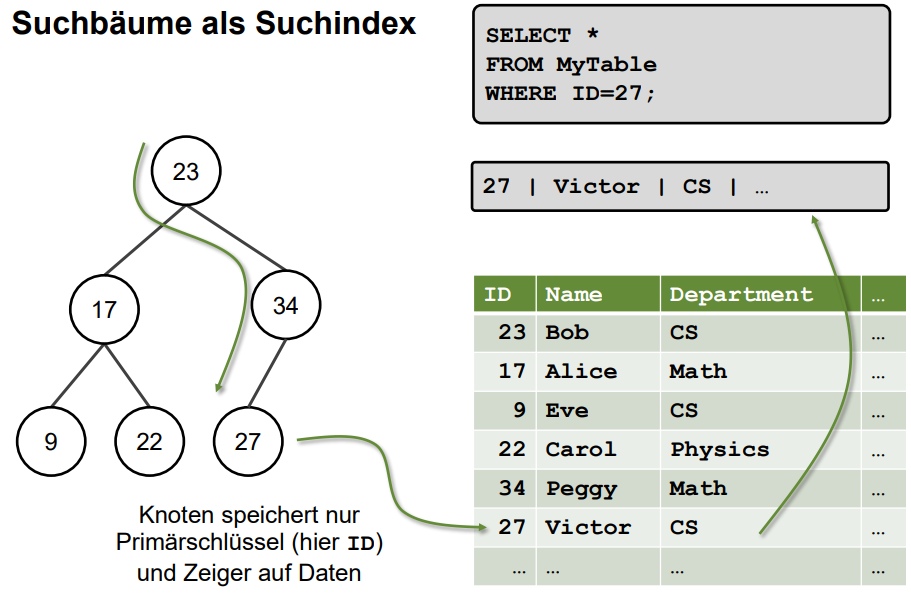
\includegraphics[width=12cm]{pictures/suchbaumSuchindex.PNG}
          \end{itemize}
\end{itemize}
\pagebreak
\end{document}

\documentclass[
    ngerman,
    color=3b,
    dark_mode,
    load_common, % Loads a list of commonly used Packages
    summary,
    boxarc,
    % manual_term,
    % solution=true,
]{tuda_summary} 
% Import all Packages from Main Preamble with relative Path
% \subimport*{../../}{preamble}
% Get Labels from Main Document using the xr-hyper Package
\externaldocument{../../AuD-Zusammenfassung-2020}
% Set Graphics Path, so pictures load correctly
\graphicspath{{../../}}


\begin{document}
\section{Advanced Data Structures}\label{Advanced Data Structures}\index{Advanced Data Structures}
\subsection{Rot-Schwarz-Bäume}\label{Rot-Schwarz-Baeume}\index{Rot-Schwarz-Bäume}
\begin{definition}[Rot-Schwarz-Baum]\mbox{}
    \begin{itemize}
        \item Ist ein binärer Suchbaum mitden zusätzlichen Eigenschaften:
              \begin{itemize}
                  \item Jeder Knoten hat die Farbe rot oder schwarz
                  \item Die Wurzel ist schwarz
                  \item Wenn ein Knoten rot ist, sind seine Kinder schwarz ("`Nicht-Rot-Rot-Regel"')
                  \item Für jeden Knoten hat jeder Pfad zu einem Blatt die selbe Anzahl an schwarzen Knoten
              \end{itemize}
        \item Halbblätter im RBT sind schwarz
        \item Schwarzhöhe\index{Schwarzhöhe} eines Knoten: \\
              Eindeutige Anzahl von schwarzen Knoten auf dem Weg zu einem Blatt im Teilbaum des Knoten
        \item Für leeren Baum gibt Schwarzhöhe = 0 ($SH(nil)=0$)
    \end{itemize}
\end{definition}
\paragraph{Höhe eines Rot-Schwarz-Baums}\mbox{}
\begin{grayInfoBox}
    \begin{itemize}
        \item $h \leq 2 \cdot log_2(n+1)$  ($n$ Knoten)
        \item In jedem Unterteilbaum gleiche Anzahl schwarzer Knoten
        \item Maximal zusätzlich gleiche Anzahl roter Knoten auf diesem Pfad
        \item Einigerma\ss{}en ausbalanciert $\Rightarrow$ Höhe $O(log~n)$
    \end{itemize}
\end{grayInfoBox}
Alle folgenden Algorithmen arbeiten mithilfe eines Sentinels (zeigt auf sich selbst)

\begin{figure}[ht]
    \centering
    \includestandalone[width=.5\textwidth]{pictures/baum_beispiel/baum_beispiel}% 
    \caption{Beispielhafte Darstellung wie in \ref{Definitionen fuer Datenstrukturen}}
    \label{fig:red_black_tree_example}
\end{figure}
\clearpage
\paragraph{Einfügen}
\begin{enumerate}
    \item Finde Elternknoten wie im BST (\hyperref[BST-Insert]{BST-Einfüge Algorithmus})
    \item Knoten als Kind von Elternknoten anfügen
    \item Färbe den neuen Knoten rot
    \item Wiederherstellen der Rot-Schwarz-Bedingung\index{fixColorsAfterInsertion()}
\end{enumerate}
%\begin{noindent}        
\begin{codeBlock}[autogobble,escapeinside=||]{title={insert(T,z) //z.left==z.right==nil;}}
    x=T.root; px=T.sent;
    WHILE x != nil DO                   //Bis zum passenden Blatt gehen
        px=x;
        IF x.key > z.key THEN
            x=x.left;
        ELSE
            x=x.right;
    z.parent=px;
    IF px==T.sent THEN                  // Einfügen
        T.root=z
    ELSE
        IF px.key > z.key THEN
            px.left=z;
        ELSE
            px.right=z;
    z.color=red;                        // ab hier anders als bei BST-Insert
    fixColorsAfterInsertion(T,z);
\end{codeBlock} 
%\end{noindent}
Laufzeit: $\Theta(h)$ ($h$ jedoch $log~n$)

Hilfsmethode \texttt{rotateLeft}\index{rotateLeft()}
%\begin{noindent}        
\begin{codeBlock}[autogobble]{title={rotateLeft(T,x)}}
    y = x.right;
    x.right = y.left;
    IF y.left != nil THEN
        y.left.parent = x;
    y.parent = x.parent;
    IF x.parent == T.sent THEN
        T.root = y;
    ELSE
        IF x == x.parent.left THEN
            x.parent.left = y;
        ELSE
            x.parent.right = y;
    y.left = x;
    x.parent = y;
\end{codeBlock}
%\end{noindent}
\clearpage
\paragraph{fixColorsAfterInsertion}
Beim Aufrufen werden zwei Bedingungen potentiell verletzt:
\begin{enumerate}
    \item root ist nicht mehr schwarz
    \item wenn eine Node rot ist müssen beide Kinder schwarz sein
\end{enumerate}
Also müssen wir:
\begin{itemize}
    \item nach Rotation die root des Baumes ggf auf schwarz setzen
    \item Überprüfen, ob RSB-Bedingung verletzt wurde
    \item Blo\ss{} wenn das parent auch rot ist kommen wir in Verlegenheit $\Longrightarrow$ wir müssen den Algorithmus starten
\end{itemize}

Fälle falls $z.parent$ rot ist:\\
\begin{minipage}{.5\textwidth-1.85301pt}
    \begin{itemize}
        \item[1.] Onkel ist ebenfalls rot $\Rightarrow$ parent und Onkel werden schwarz gefärbt und Grandparent wird rot gefärbt, z wird zu z.p.p, ggf. Verletzung durch Farbe des neuen z
        \item[2.] Onkel ist schwarz und z hat andere Kindrichtung wie z.p $\Rightarrow$ zu Fall 3 durch Rotation konvertieren
        \item[3.] Onkel ist schwarz und z hat gleiche Kindrichtung wie z.p $\Rightarrow$ z.p wird schwarz, z.p.p wird rot, und es wird um z.p.p entgegen der Kindrichtung gedreht. Schleife terminiert nach Fall 3
    \end{itemize}
\end{minipage}
\begin{minipage}{.5\textwidth}
    \begin{tcolorbox}[
            colback=yellow!20,
            colframe=black!70,
            enhanced,
            title={Fall 1},
            fonttitle=\sffamily\bfseries,
            center title,
            every float=\centering
        ]
        \centering
        \includestandalone{pictures/fixColorsAfterInsertionCases/case1}
    \end{tcolorbox}
\end{minipage}\\
\begin{minipage}[t]{.5\textwidth}\mbox{}
    \begin{tcolorbox}[
            colback=yellow!20,
            colframe=black!70,
            enhanced,
            title={Fall 2},
            fonttitle=\sffamily\bfseries,
            center title,
            every float=\centering
        ]
        \centering
        \includestandalone{pictures/fixColorsAfterInsertionCases/case2}
    \end{tcolorbox}
    %\captionof*{figure}{Fall 2}
\end{minipage}
\begin{minipage}[t]{.5\textwidth-1.85301pt}\mbox{}
    \begin{tcolorbox}[
            colback=yellow!20,
            colframe=black!70,
            enhanced,
            title={Fall 3},
            fonttitle=\sffamily\bfseries,
            center title,
            every float=\centering,
        ]
        \centering
        \includestandalone{pictures/fixColorsAfterInsertionCases/case3}
    \end{tcolorbox}
    %\captionof*{figure}{Fall 3}
\end{minipage}
%\begin{noindent}
        \begin{codeBlock}[autogobble,fontsize=\small]{title={fixColorsAfterInsertion(T,z)}}
            WHILE z.parent.color == red DO                  // solange der Elternknoten rot ist
                IF z.parent == z.parent.parent.left THEN    // Linkes Kind (if-Fall)
                    y = z.parent.parent.right;
                    IF y != nil AND y.color == red THEN     // Fall 1
                        z.parent.color = black;
                        y.color = black;
                        z.parent.parent.color = red;
                        z = z.parent.parent;                // rekursiv nach oben weiterführen
                    ELSE                                    
                        IF z == z.parent.right THEN         // Fall 2
                            z = z.parent;
                            rotateLeft(T,z);
                        z.parent.color = black;             // Fall 3
                        z.parent.parent.color = red;
                        rotateRight(T, z.parent.parent);
                ELSE                                        
                    // Tauschen von rechts und links        
                T.root.color = black;                       // Setzen der Wurzel auf Schwarz
            \end{codeBlock}
            %\end{noindent}
\clearpage
\paragraph{Löschen}
\begin{itemize}
    \item analog zum binären Suchbaum, aber neue Node erbt Farbe der alten Node
    \item Wenn "`neue"' Node schwarz war $\Rightarrow$ Fixup
    \item Verschiedene Fälle, die auch gegenseitig Voraussetzungen füreinander sind
\end{itemize}
Hilfsroutine transplant:\index{transplant}
%\begin{noindent}
\begin{codeBlock}[autogobble,fontsize=\small]{title={transplant(T,u,v)}}
    IF u.parent==nil THEN
        T.root=v;
    ELSE
        IF u==u.parent.left THEN
            u.parent.left=v;
        ELSE
            u.parent.right=v;
    IF v != nil THEN
        v.parent=u.parent;
\end{codeBlock}
%\end{noindent}
%\begin{noindent}
\begin{codeBlock}[autogobble,fontsize=\small]{title={delete(T,z)}}
    y=z;
    y-original-color=y.color;
    IF z.left == nil;
        x = z.right;
        transplant(T,z,z.right);
    ELSE IF z.right == nil;
        x = z.left;
        transplant(T,z,z.left);
    ELSE
        y TREE-MINIMUM(z.right);
        y-original-color=y.color;
        x=y.right;
        IF y.p == z
            x.p = y;
        ELSE
            transplant(T,y,y.right);
            y.right=z.right;
            y.right.p=y;
        transplant(T,z,y);
        y.left=z.left;
        y.left.p=y;
        y.color=z.color;
    IF y-original-color == BLACK
        deleteFixup(T,x);
\end{codeBlock}
%\end{noindent}
Laufzeit: $O(h) = O(log~n)$
\clearpage
Delete kann die RSB-Bedingung verletzen. Das fixup hat vier fälle:
\begin{figure}[h]
    \centering
    \includegraphics[width=\textwidth-2cm]{pictures/deleteFixuoRBTCases\IfDarkModeT{_dark}.png}
    \caption{Fälle für Fixup bei delete in RSB}
\end{figure}
\begin{enumerate}
    \item Knoten $w$ (Bruder von Knoten $x$) ist rot
          \begin{itemize}
              \item Da $w$ schwarze Kinder haben muss, können wir die Farben von $w$ und $x.p$ wechseln und dann eine Linksdrehung auf $x.p$ ausführen, ohne eine der rot-schwarzen Eigenschaften zu verletzen.
              \item Das neue Geschwisterchen von $x$, das vor der Rotation eines der Kinder von $w$ ist, ist jetzt schwarz. Wir haben also Fall $1$ in Fall $2, 3$ oder $4$ konvertiert.
                    Die Fälle $ 2, 3$ und $4$ treten auf, wenn der Knoten $w$ schwarz ist, aber unterschiedliche Farben der Kinder.
          \end{itemize}
    \item $w$ ist schwarz und beide Kinder von $w$ sind schwarz
          \begin{itemize}
              \item entfernen eines Schwarz von $x$ und $w$, wobei $x$ nur ein Schwarz hat und $w$ rot bleibt
              \item Um Entfernen aus $x$ und $w$ zu kompensieren ein zusätzliches Schwarz hinzufügen.
              \item w konnte entweder Schwarz oder rot sein.
              \item Wenn $x.p~(=a)$ schwarz, dann Vaterknoten $\Delta SH=-1$; verfahre rekursiv mit $x.p~(=a)$ als neuem $x$; $\Rightarrow$ wir wiederholen die while-Schleife mit $x.p$ als neuem Knoten $x$.
          \end{itemize}
    \item $w$ ist schwarz, $w$'s linkes Kind ist rot und $w$'s rechtes Kind ist schwarz
          \begin{itemize}
              \item Farben von $w$ und seinem linken Kind links ändern und dann eine Rechtsdrehung auf $w$ ausführen
              \item Das neue Geschwister $w$ von $x$ ist jetzt ein schwarzer Knoten mit einem roten rechten Kind
              \item[$\Rightarrow$] Fall $3$ in Fall $4$ transformiert.
          \end{itemize}
    \item $w$ ist schwarz und das rechte Kind von $w$ ist rot
          \begin{itemize}
              \item $w$ erbt die Farbe von $x.p$
              \item $x.p$ wird schwarz
              \item $w.right$ wird schwarz
              \item[$\Rightarrow$] LinksRotation von $x.p$
              \item $x$ als Wurzel festlegen, wird der Whileloop beendet, wenn die Schleifenbedingung getestet wird.
          \end{itemize}
\end{enumerate}

%\begin{noindent}
                \begin{codeBlock}[autogobble,fontsize=\small]{title={deleteFixup(T,z)}}
                    WHILE x != T.root and x.color == BLACK
                        IF x==x.p.left
                            w=x.p.right;
                            IF w.color == RED                           // Case 1
                                w.color=BLACK;
                                x.p.color=RED;
                                rotateLeft(T,x.p);
                                w=x.p.right;
                            IF w.left.color == w.right.color == BLACK   // Case 2
                                w.color = RED;
                                x=x.p;
                            ELSE IF w.right.color == BLACK              // Case 3
                                w.left.color = BLACK;
                                w.color=RED;
                                rotateRight(T,w);
                                w=x.p.right;
                            w.color=x.p.color;                          // Case 4
                            x.p.color=BLACK;
                            w.right.color=BLACK;
                            rotateLeft(T,x.p);
                            x=T.root;
                        ELSE
                            // same as above with "right" and "left" exchanged
                    x.color=BLACK;
                \end{codeBlock}
                %\end{noindent}

\paragraph{Worst-Case-Laufzeiten}
\begin{description}[leftmargin=2cm]
    \item [Einfügen] $\Theta(log~n)$
    \item [Löschen] $\Theta(log~n)$
    \item [Suchen] $\Theta(log~n)$
\end{description}
\clearpage
\subsection{AVL-Bäume}\label{AVL-Baeume}\index{AVL-Bäume}
\begin{wrapfigure}[5]{r}{.4\textwidth}
    % \centering
    \includegraphics[width=7cm]{pictures/avlbaum\IfDarkModeT{_dark}.PNG}
    \caption{Beispiel Balance AVL Baum}
\end{wrapfigure}\mbox{}
\begin{definition}[AVL-Baum]\mbox{}\\
    Binärer Suchbaum, aber für Balance in \fatsf{jedem} Knoten nur $-1,0,$ oder $1$ erlaubt.\\
    Balance für $x$: $B(x)$ = Höhe(rechter Teilbaum) - Höhe(linker Teilbaum)
    \index{linkslastig}\index{rechtslastig}\index{balanciert}
\end{definition}
$h \leq 1.441 \cdot log~n$ (optimierte Konstanten - 1,441 vs 2 (RBT))\\
\paragraph{AVL vs. Rot-Schwarz-Bäume}\mbox{}
\begin{grayInfoBox}
    \begin{description}[leftmargin=3cm,itemsep=1em]
        \item [AVL]
              \begin{itemize}
                  \item Einfügen und Löschen verletzen in der Regel öfter die Baum-Bedingung
                  \item Aufwendiger zum Rebalancieren
              \end{itemize}
        \item [Rot-Schwarz]
              \begin{itemize}
                  \item Suchen dauert evtl. länger
              \end{itemize}
        \item [Konklusion]
              \begin{itemize}
                  \item AVL geeigneter, wenn mehr Such-Operationen und weniger Einfügen und Löschen
              \end{itemize}
        \item [Gemeinsamkeiten]\begin{itemize}
                  \item AVL $\subset$ Rot-Schwarz
                  \item AVL-Baum $\Rightarrow$ Rot-Schwarz-Baum mit Höhe $\left \lceil \frac{h+1}{2} \right \rceil$
                  \item Für jede Höhe $h \geq 3$ gibt es einen RBT, der kein AVL-Baum ist (AVL $\neq$ RBT)
              \end{itemize}
    \end{description}
\end{grayInfoBox}
\clearpage
\paragraph{Einfügen}
\begin{itemize}
    \item Einfügen funktioniert wie beim Binary Search Tree mit Sentinel\index{Sentinel}
    \item Erfordert danach jedoch Rebalancieren weiter oben im Baum
    \item Rebalancieren: (verschiedene Fälle)
\end{itemize}

\begin{minipage}{0.5\textwidth}
    \centering\includegraphics[width=\textwidth]{pictures/avlcase1\IfDarkModeT{_dark}.PNG}
\end{minipage}
\begin{minipage}{0.5\textwidth}
    \centering\includegraphics[width=\textwidth]{pictures/avlcase34\IfDarkModeT{_dark}.PNG}
\end{minipage}

\begin{minipage}{0.5\textwidth}
    \centering\includegraphics[width=\textwidth]{pictures/avlcase2_1\IfDarkModeT{_dark}.PNG}
\end{minipage}
\begin{minipage}{0.5\textwidth}
    \centering\includegraphics[width=\textwidth]{pictures/avlcase2_2\IfDarkModeT{_dark}.PNG}
\end{minipage}


\paragraph{Löschen}
\begin{itemize}
    \item Analog zum binären Suchbaum
    \item Rebalancieren (eventuell bis zur Wurzel) notwendig
\end{itemize}

\paragraph{Worst-Case-Laufzeiten}
\begin{itemize}
    \item {\makebox[2cm][l]{Einfügen: }} $\Theta(log~n)$
    \item {\makebox[2cm][l]{Löschen: }} $\Theta(log~n)$
    \item {\makebox[2cm][l]{Suchen: }} $\Theta(log~n)$
    \item theoretisch bessere Konstanten als RBT
    \item in Praxis aber nur unwesentlich schneller
\end{itemize}
\clearpage
\subsection{Splay-Bäume}\label{Splay-Baeume}\index{Splay-Bäume}
\begin{definition}[Splay-Baum]
    \begin{itemize}
        \item selbst-organisierender Baum
        \item Ansatz: Einmal angefragte Werte werden wahrs. noch öfter angefragt
        \item Angefragte Werte nach oben schieben
        \item Splay-Bäume sind eine Untermenge von Rot-Schwarz-Bäumen ($\subseteq$)
    \end{itemize}
\end{definition}

\paragraph{Splay-Operationen}
\begin{itemize}
    \item Suchen oder Einfügen: Spüle gesuchten oder neu eingefügten Knoten an die Wurzel
    \item Splay:\index{splay} Folge von Zig-,Zig-Zig-, Zig-Zag-Operationen
\end{itemize}
%\begin{noindent}
\begin{codeBlock}[autogobble]{title={splay(T,z)}}
WHILE z != T.root DO
    IF z.parent.parent == nil THEN
        zig(T,z);
    ELSE
        IF z == z.parent.parent.left.left OR
           z == z.parent.parent.right.right THEN
           zigZig(T,z);
        ELSE
            zigZag(T,z);
\end{codeBlock}
%\end{noindent}

\index{Zig-Zag} \includegraphics[width=12cm]{pictures/zigzag\IfDarkModeT{_dark}.PNG}\\
\index{Zig-Zig} \includegraphics[width=11cm]{pictures/zigzig\IfDarkModeT{_dark}.PNG}\vspace{1em}\\
\index{Zig} \includegraphics[width=11cm]{pictures/zig\IfDarkModeT{_dark}.PNG}\\

\vspace*{-1em}
\begin{description}[itemsep=.8em]
    \item[Suchen] \begin{itemize}
              \item Laufzeit: $O(h)$
              \item Suche des Knotens wie im BST
              \item Hochspülen des gefundenen Knotens (alternativ zuletzt besuchter Knoten, falls nicht gefunden)
          \end{itemize}
    \item[Einfügen] \begin{itemize}
              \item Laufzeit: $O(h)$
              \item Suche der Position wie im BST
              \item Einfügen und danach hochspülen des eingefügten Knotens
          \end{itemize}
    \item[Löschen] \begin{itemize}
              \item Laufzeit: $O(h)$
              \item[1.] Spüle gesuchten Knoten per Splay-Operation nach oben
              \item[2.] Lösche den gesuchten Knoten (Wenn einer der beiden entstehenden Teilbäume leer, dann fertig)
              \item[3.] Spüle den grö\ss{}ten Knoten im linken Teilbaum nach oben (kann kein rechtes Kind haben)
              \item[4.] Hänge rechten Teilbaum an grö\ss{}ten Knoten aus 3. an
          \end{itemize}
    \item[Laufzeit Splay-Bäume] \begin{itemize}
              \item Amortisierte Laufzeit: Laufzeit pro Operation über mehrere Operationen hinweg
              \item Worst-Case-Laufzeit pro Operation: $O(log_n~n)$
          \end{itemize}
\end{description}

\clearpage
\subsection{Binäre Max-Heaps}\label{Binaere Max-Heaps}\index{Binäre Max-Heaps}
\begin{definition}[Binäre Max-Heaps]\mbox{}
    \begin{itemize}
        \item Heaps sind keine BSTs
        \item Eigenschaften von binären Max-Heaps:
              \begin{itemize}
                  \item bis auf das unterste Level vollständig und dort von links gefüllt ist
                  \item Für alle Knoten gilt: \texttt{x.parent.key $\geq$ x.key}
                  \item Maximum des Heaps steht damit in der Wurzel
              \end{itemize}
        \item $h \leq log~n$, da Baum fast vollständig
    \end{itemize}
\end{definition}

\paragraph{Heaps durch Arrays}\mbox{}\\
\includegraphics[width=8cm]{pictures/heapArr\IfDarkModeT{_dark}.PNG}

\paragraph{Einfügen}\mbox{}
\begin{idea}[Einfügen]
    Einfügen und danach Vertauschen nach oben, bis Max-Eigenschaft wieder erfüllt ist
\end{idea}

Code:
%\begin{noindent}
\begin{codeBlock}[autogobble]{title={insert(H,k) // als unbeschränktes Array}}
H.length = H.length + 1;
H.A[H.length-1] = k;
i = H.length - 1;
WHILE i > 0 AND H.A[i] > H.A[i.parent]
    SWAP(H.A, i, i.parent);
    i = i.parent;
\end{codeBlock}
%\end{noindent}
Laufzeit: $O(h) = O(log~n)$
\clearpage
\paragraph{Lösche Maximum}
\begin{enumerate}
    \item[1.] Ersetze Maximum durch "`letztes"' Blatt
    \item[2.] Vertausche Knoten durch Maximum der beiden Kinder (\texttt{heapify})
\end{enumerate}
\index{extract-max(H)}\index{heapify(H,i)}
\begin{minipage}[t]{0.57\textwidth}\mbox{}
    %\begin{noindent}
    \begin{codeBlock}[autogobble]{title={extract-max(H)}}
    IF isEmpty(H) THEN return error "underflow";
    ELSE
        max = H.A[0];
        H.A[0] = H.A[H.length - 1];
        H.length = H.length - 1;
        heapify(H, 0);
        return max;
    \end{codeBlock}
    %\end{noindent}
\end{minipage}
\begin{minipage}[t]{0.43\textwidth}\mbox{}
    \centering
    \includegraphics[width=\textwidth]{pictures/heapDelete\IfDarkModeT{_dark}.PNG}
    \captionof{figure}{Beispiel Löschen des Maximums im Binären Max-Heap}
\end{minipage}

%\begin{noindent}
\begin{codeBlock}[autogobble]{title={heapify(H, i)}}
maxind = i;
IF i.left < H.length AND H.A[i]<H.A[i.left] THEN
    maxind = i.left;
IF i.right < H.length AND H.A[maxind]<H.A[i.right] THEN
    maxind = i.right;
IF maxind != i THEN
    SWAP(H.A, i, maxind);
    heapify(H, maxind);
\end{codeBlock}
%\end{noindent}

\paragraph{Heap-Konstruktion aus Array}
\begin{itemize}
    \item Blätter sind für sich triviale Max-Heaps
    \item Bauen von Max-Heaps für Teilbäume mithilfe Rekursion per \texttt{heapify}
    \item (Array nicht unbedingt in richtiger Reihenfolge)
\end{itemize}
\index{buildHeap(H,A)}\index{HeapSort(H,A)}
%\begin{noindent}
\begin{codeBlock}[autogobble]{title={buildHeap(H.A) // Array in H.A}}
    H.length = A.length;
    FOR i = ceil((H.length-1)/2) - 1 DOWNTO 0 DO
        heapify(H.A,i);
\end{codeBlock}
%\end{noindent}


\paragraph{Heap-Sort}
\begin{itemize}
    \item Idee: Bauen des Heaps aus Array und dann (wiederholte) Extraktion des Maximums
\end{itemize}
%\begin{noindent}
\begin{codeBlock}[autogobble]{title={heapSort(H.A)}}
buildHeap(H.A)                  // Bauen des Heaps
WHILE !isEmpty(H) DO
    PRINT extract-max(H);       // Ausgabe des Maximums bis Heap leer ist
\end{codeBlock}
%\end{noindent}

\clearpage
\subsection{B-Bäume}\label{B-Baeume}\index{B-Baeume}
\begin{definition}[B-Baum]\mbox{}
    \begin{itemize}
        \item Jeder B-Baum hat einen angebenen Grad also z.B. $t=2$
        \item Eigenschaften:
              \begin{itemize}
                  \item Wurzel zwischen $[1,~\cdots,~2t-1]$ Werte
                  \item Knoten zwischen $[t-1,~\cdots,~2t-1]$ Werte
                  \item Werte innerhalb eines Knotens aufsteigend geordnet
                  \item Blätter haben alle die gleiche Höhe
                  \item Jeder innere Knoten mit $n$ Werten hat $n+1$ Kinder, sodass gilt:
                  \item[] $k_0 \leq key[0] \leq k_1 \leq key[1] \leq ... \leq k_{n-1} \leq key[n-1] \leq k_n$
              \end{itemize}
    \end{itemize}
\end{definition}

\includegraphics[width=15cm]{pictures/bbaum\IfDarkModeT{_dark}.PNG}
\begin{grayInfoBox}
    \begin{itemize}
        \item Höhe B-Baum: $h \leq log_t \frac{n+1}{2}$ (Grad $t$ und $n$ Werte)
        \item B-Baum wird für grö\ss{}ere $t$ flacher
    \end{itemize}
\end{grayInfoBox}
\clearpage
\paragraph{Suche}\mbox{}\\
\includegraphics[width=12cm]{pictures/bbaumSuche\IfDarkModeT{_dark}.PNG}
%\begin{noindent}
\begin{codeBlock}[autogobble]{title={search(x, k)}}
WHILE x != nil DO
    i = 0;
    WHILE i < x.n AND x.key[i] < k DO
        i++;
    IF i < x.n AND x.key[i] == k THEN
        return(x, i);
    ELSE
        x = x.child[i];
return nil;
\end{codeBlock}
%\end{noindent}


\paragraph{Einfügen}
\begin{itemize}
    \item Einfügen erfolgt immer in einem Blatt
    \item Falls das Blatt voll ist, muss jedoch gesplittet werden
    \item $\Rightarrow$ Beim Durchlaufen des Baumes an jeder notwendigen vollen Position splitten
    \item Splitten:\index{Splitten}
          \begin{itemize}
              \item Bricht volle Node auf und fügt mittleren Wert zur Elternnode hinzu
              \item Aus den anderen Werten entstehen nun jeweils eigene Kinder
              \item An der Wurzel splitten erzeugt neue Wurzel und erhöht Baumhöhe um eins
          \end{itemize}
    \item Ablauf zusammengefasst:
          \begin{enumerate}
              \item Start bei Wurzel, falls kein Platz mehr splitten
              \item Durchlaufen des Baumes bis zur richtigen Position und immer, falls voll, splitten
              \item Einfügen der Node (fertig)
          \end{enumerate}
\end{itemize}
%\begin{noindent}
\begin{codeBlock}[autogobble]{title={insert(T, z)}}
Wenn Wurzel schon 2t-1 Werte hat, dann splitte Wurzel
Suche rekursiv Einfügeposition:
    Wenn zu besuchendes Kind 2t-1 Werte hat, splitte es erst
Füge z in Blatt ein
\end{codeBlock}
%\end{noindent}


\clearpage

\paragraph{Löschen}
\begin{itemize}
    \item Wenn Blatt noch mehr als $t-1$ Werte, kann der Wert einfach entfernt werden
    \item Allerdings durchlaufen wir hier den Baum auch wieder von oben und stellen gewisse Voraussetzungen her
    \item Durchlaufen des Baumes von oben und Anwendung der folgenden Algorithmen
\end{itemize}
\begin{minipage}{0.25\textwidth}
    \includegraphics[width=4cm]{pictures/bbaumMelt\IfDarkModeT{_dark}.PNG}
\end{minipage}
\begin{minipage}{0.75\textwidth}
    Allgemeines Verschmelzen:\index{Verschmelzen}
    \begin{itemize}
        \item Kind und rechter und linker Geschwisterknoten (sofern existent) nur $t-1$ Werte
        \item Wenn Elternknoten vorher min. $t$ Werte
        \item[] $\Rightarrow$ keine Änderung oberhalb notwendig
    \end{itemize}
\end{minipage} \vspace{1em}\\
\begin{minipage}{0.25\textwidth}
    \includegraphics[width=4cm]{pictures/bbaumRot\IfDarkModeT{_dark}.PNG}
\end{minipage}
\begin{minipage}{0.75\textwidth}
    Allgemeines Rotieren/Verschieben:
    \begin{itemize}
        \item Kind nur $t-1$ Werte
        \item Geschwister jedoch mehr als $t-1$ Werte
        \item keine Änderung oberhalb notwendig
    \end{itemize}
\end{minipage}

Code:

%\begin{noindent}
                    \begin{codeBlock}[autogobble]{title={delete(T, k)}}
                    Wenn Wurzel nur 1 Wert und beide Kinder t-1 Werte, 
                    verschmelze Wurzel und Kinder (reduziert Höhe um 1)
                    Suche rekursiv Löschposition:
                        Wenn zu besuchendes Kind nur t-1 Werte, 
                        verschmelze es oder rotiere/verschiebe
                    Entferne Wert k im inneren Knoten/Blatt             
                    // Ohne Probleme, aufgrund vorheriger Anpassung
                    \end{codeBlock}
                %\end{noindent}


\paragraph{Laufzeiten}
\begin{description}[leftmargin=2cm]
    \item [Einfügen] $\Theta(log_t~n)$
    \item [Löschen] $\Theta(log_t~n)$
    \item [Suchen] $\Theta(log_t~n)$
\end{description}
\begin{itemize}
    \item Nur vorteilhaft wenn Daten blockweise eingelesen werden
    \item $\mathcal{O}$-Notation versteckt hier konstanten Faktor $t$ für Suche innerhalb eines Knotens
\end{itemize}
\clearpage
\end{document}

\documentclass[
    12pt,
    a4paper,
    ngerman,
    color=3b,% Farbe für Hervorhebungen auf Basis der Deklarationen in den
    %type=intern,
    %titlepage=true,
    marginpar=false,
    colorback=false,
    %logo=head,
    leqno,
]{tudaexercise}
\usepackage{import}
% Import all Packages from Main Preamble with relative Path
\subimport*{../../}{preamble}
% Get Labels from Main Document using the xr-hyper Package
\externaldocument{../../AuD-Zusammenfassung-2020}
% Set Graphics Path, so pictures load correctly
\graphicspath{{../../}}


\begin{document}
\section{Randomized Data Structures}\label{Randomized Data Structures}\index{Randomized Data Structures}
\subsection{Skip Lists}\label{Skip Lists}\index{Skip Lists}
    \begin{itemize}
        \item \fatsf{Idee}
            \begin{itemize}
                \item Einfügen von "`Express-Liste"'\index{Express-Liste} mit einigen Elementen
                \item Beginne mit Suche in der Express-Liste mit weniger Elementen
                \item Falls das suchende Element kleiner als nächstes Element in Express-Liste $\Rightarrow$ weiter nach rechts
                \item Falls nicht $\Rightarrow$ Eine Stufe nach unten wandern und dort weiter suchen
                \item[] \includegraphics[width=12cm]{pictures/skiplistSuche.PNG}
                \item Verbesserung: Zusätzliche Stufen an Express-Listen 
                \item Anwendung: 
                \begin{itemize}
                    \item Gut für parallele Verarbeitung z.B. Multicore-Systeme (Einfügen und Löschen)
                    \item Dafür logarithmische Laufzeit nur im Durchschnitt
                \end{itemize}
                \item Auswahl von Elementen:
                    \begin{itemize}
                        \item Abhängig von einer gewählten Wahrscheinlichkeit $p$ 
                        \item Element kommt mit Wahrscheinlichkeit $p$ in übergeordnete Liste
                        \item Höhe: $h = O(log_{\frac{1}{p}}n)$
                        \item Anzahl Elemente: $n \Rightarrow pn \Rightarrow p^2n \Rightarrow ...$ (unten nach oben)
                    \end{itemize}
            \end{itemize}

        \item \fatsf{Implementierung}
            \begin{itemize}
                \item[]
                        \includegraphics[width=12cm]{pictures/skiplistImplement1.PNG}\\
                        \includegraphics[width=8cm]{pictures/skiplistImplement2.PNG}
            \end{itemize}
\clearpage
        \item \fatsf{Suche}
            \begin{itemize}
                \item Laufzeit ist von Expresslisten abhängig
                \item[]
                    \begin{ccode}[autogobble]{title={search(L, k)}}
                    current = L.head;
                    WHILE current != nil DO
                        IF current.key == k THEN 
                            return current;
                        IF current.next != nil AND current.next.key <= k THEN
                            current = current.next;
                        ELSE
                            current = current.down;
                    return nil;
                    \end{ccode}
            \end{itemize}

        \item \fatsf{Einfügen}
            \begin{itemize}
                \item Füge auf unterster Ebene ein
                \item Evtl. auf höheren Ebenen mit zufälliger Wahl mithilfe von $p$ auf jeder Ebene
            \end{itemize}

        \item \fatsf{Löschen}
            \begin{itemize}
                \item Entferne Vorkommen des Elements aus allen Ebenen
            \end{itemize}
        
        \item \fatsf{Laufzeiten}
            \begin{itemize}
                \item {\makebox[2cm][l]{Einfügen: }} $\Theta(log_{\frac{1}{p}}n)$
                \item {\makebox[2cm][l]{Löschen: }} $\Theta(log_{\frac{1}{p}}n)$
                \item {\makebox[2cm][l]{Suchen: }} $\Theta(log_{\frac{1}{p}}n)$
                \item (Im Durchschnitt)
                \item $O$-Notation versteckt konstanten Faktor $\frac{1}{p}$
                \item Speicherbedarf im Durchschnitt: $\frac{n}{1-p}$
            \end{itemize}
    \end{itemize}
\clearpage
\subsection{Hashtables}\label{Hashtables}\index{Hashtables}
    \begin{itemize}
        \item \fatsf{Idee}
            \begin{itemize}
                \item[]
                    \begin{minipage}{0.4\textwidth}
                        \includegraphics[width=5cm]{pictures/hashtableIdee.PNG}
                    \end{minipage}
                    \begin{minipage}{0.5\textwidth}
                        \begin{itemize}
                            \item Hashfunktion sollte gut verteilen
                            \item $h(x)$ sollte uniform sein
                            \item Unabhängig im Intervall $[0, T.length-1]$ verteilt
                            \item Einfügen mit konstant vielen Array-Operationen
                        \end{itemize}
                    \end{minipage}
                \item[]
                \item[]
                \item[]
                    \begin{minipage}{0.4\textwidth}
                        \includegraphics[width=5cm]{pictures/hashtableLinkedList.PNG}
                    \end{minipage}
                    \begin{minipage}{0.5\textwidth}
                        \begin{itemize}
                            \item Kollisionsauflösung z.B. mithilfe von LinkedLists
                            \item Neue Elemente werden vorne angefügt
                            \item Konstante Anzahl an Array-Operationen
                            \item Soviele Schritte wie die Liste lang ist 
                            \item Uniforme Hashfunktion
                            \item[] $\Rightarrow$ $\frac{n}{T.length}$ Einträge pro Liste
                        \end{itemize}
                    \end{minipage}
                \item[]
            \end{itemize}

        \item \fatsf{Hash-Funktionen}\index{Hash-Funktion}
            \begin{itemize}
                \item Universelle Hash-Funktion\index{Hash-Funktion!universell}:
                    \begin{itemize}
                        \item Wähle zufällige $a,b \in [0, p - 1]$, $p~prim$, $a \neq 0$
                        \item $h_{a,b}(x)= ((a \cdot x + b)~mod~p)~mod~T.length$
                    \end{itemize}
                \item Krypthographische Hash-Funktionen:\index{Hash-Funktion!Kryptographisch}
                    \begin{itemize}
                        \item MD5, SHA-1, SHA-2, SHA-3
                        \item $h(x) = MD5(x)~mod~T.length$
                    \end{itemize}
            \end{itemize}

\pagebreak
        
        \item \fatsf{Hashtables vs. Bäume}
            \begin{itemize}
                \item Hashtables:
                    \begin{itemize}
                        \item nur Suche nach bestimmten Wert möglich
                        \item meist größer als zu erwartende Anzahl Einträge
                    \end{itemize}
                \item Bäume:
                    \begin{itemize}
                        \item schnelles Traversieren zu Nachbarn möglich
                        \item Bereichssuche möglich
                    \end{itemize}
            \end{itemize}
        
        \item \fatsf{Laufzeiten}
            \begin{itemize}
                \item Wählt mal $T.length = n$ ergibt sich konstante Laufzeit
                \item {\makebox[2cm][l]{Einfügen: }} $\Theta(1)$
                \item {\makebox[2cm][l]{Löschen: }} $\Theta(1)$
                \item {\makebox[2cm][l]{Suchen: }} $\Theta(1)$
                \item (Im Durchschnitt, beim Einfügen sogar im Worst-Case)
                \item Speicherbedarf i.d.R. höher als n, meist ca. $1,33 \cdot n$
            \end{itemize}
    \end{itemize}

\subsection{Bloom-Filter}\label{Bloom-Filter}\index{Bloom-Filter}
    \begin{itemize}
        \item \fatsf{Idee}
            \begin{itemize}
                \item Speicherschonende Wörterbucher mit kleinem Fehler
                \item z.B. Vermeidung von schlechten Passwörtern 
                    \begin{enumerate}
                        \item Abspeichern aller schlechten Passwörter in kompakter Form
                        \item Prüfe, ob eingegebenes Passwort im Bloom-Filter
                    \end{enumerate}
                \item z.B. Erkennen von schädlichen Websites (Chrome früher)
            \end{itemize}

        \item \fatsf{Erstellen}
            \begin{itemize}
                \item $n$ Elemente $x_0,...,x_{n-1}$
                \item $m$ Bits-Speicher z.B. als Bit-Array
                \item $k$ gute Hash-Funktionen $H_0,...,H_{k-1}$ mit Bildbereich $0,1,...,m-1$
                \item Empfohlene Wahl: $k = \frac{m}{n} \cdot ln2$ (Fehlerrate von ca. $2^{-k}$)
                \clearpage
                \item Code:\index{initBloom(X,BF,H)}
                \item[]
                    \begin{ccode}[autogobble]{title={initBloom(X, BF, H) // H Array of hash functions}}
                    FOR i = 0 TO BF.length - 1 DO 
                        BF[i] = 0;
                    FOR i = 0 TO X.length - 1 DO
                        FOR j = 0 TO H.length - 1 DO
                            BF[H[j](X[i])] = 1;
                    \end{ccode}
                \item[]
                \item[1.] Initialisiere Array mit 0-Einträgen
                \item[2.] Schreibe für jedes Element in jede Bit-Position $H_0(x_i),...,H_{k-1}(x_i)$ eine 1 
                \item[] \includegraphics[width=15cm]{pictures/bloomCreate.PNG} 
            \end{itemize}

        \item \fatsf{Suche}
            \begin{itemize}
                \item[]\index{searchBloom(BF,H,y)}
                    \begin{ccode}[autogobble]{title={searchBloom(BF, H, y)}}
                    result = 1;
                    FOR j = 0 TO H.length - 1 DO
                        result = result AND BF[H[j](y)];
                    return result;
                    \end{ccode}
                \item[]
                \item Gibt an, dass $y$ im Wörterbuch, falls alle $k$ Einträge für $y$ in $BF=1$ sind
                \item[] \includegraphics[width=13.5cm]{pictures/bloomSearch.PNG}
                \item Eventuell \string"false positives\string" (1, obwohl $y$ nicht im Wörterbuch)
                    \begin{itemize}
                        \item Passiert, falls die Einträge vorher von anderen Werten getroffen wurden
                        \item Daher gute Hashfunktionen und Filtergrö\ss e nicht zu klein
                    \end{itemize}
            \end{itemize}
    \end{itemize}
    \clearpage
\end{document}

\documentclass[
    12pt,
    a4paper,
    ngerman,
    color=3b,% Farbe für Hervorhebungen auf Basis der Deklarationen in den
    %type=intern,
    %titlepage=true,
    marginpar=false,
    colorback=false,
    %logo=head,
    leqno,
]{tudaexercise}
\usepackage{import}
% Import all Packages from Main Preamble with relative Path
\subimport*{../../}{preamble}
% Get Labels from Main Document using the xr-hyper Package
\externaldocument{../../AuD-Zusammenfassung-2020}
% Set Graphics Path, so pictures load correctly
\graphicspath{{../../}}

\begin{document}
\section{Graph Algorithms}
\subsection{Graphen}
    \begin{itemize}
        \item \fatsf{(Endlicher) gerichteter Graph}
            \begin{itemize}
                \item (endlicher) gerichteter Graph $G = (V,E)$
                \item besteht aus (endlicher) Knotenmenge $V$
                \item besteht aus (endlicher) Kantenmenge $E \subseteq V x V$
                \item $(u,v) \in E$: Kanten von Knoten $u$ zu $v$
                \item Kanten haben eine Richtung
            \end{itemize}

        \item \fatsf{Ungerichtete Graphen}
            \begin{itemize}
                \item (endlicher) ungerichteter Graph $G = (V,E)$
                \item besteht aus (endlicher) Knotenmenge $V$
                \item besteht aus (endlicher) Kantenmenge $E \subseteq V x V$, sodass $(u,v) \in E \Leftrightarrow (v,u) \in E$
                \item Kanten haben keine Richtung
            \end{itemize}

        \item \fatsf{Pfadfinder}
            \begin{itemize}
                \item Knoten $v$ ist von Knoten $u$ erreichbar, wenn es einen Pfad gibt
                \item $u$ ist immer von $u$ per leerem Pfad (k=1) erreichbar
                \item Länge des Pfades = $k - 1$ = Anzahl Kanten
            \end{itemize}

        \item \fatsf{Zusammenhänge}
            \begin{itemize}
                \item Ungerichtet: Zusammenhängend wenn jeder Knoten von jedem anderen Knoten aus erreichbar ist
                \item Gerichtet: \fatsf{Stark} zusammenhängend, wenn obiges auch gemäß Kantenrichtung gilt
            \end{itemize}

        \item \fatsf{Bäume und Subgraphen} \\
            Graph $G$ ist ein Baum, wenn $V$ leer ist oder wenn es einen Knoten in $V$ gibt, \\
            von dem aus jeder andere Knoten eindeutig erreichbar ist (Wurzel). \\
            Graph $G'=(V',E')$ ist Subgraph von $G=(V,E)$, wenn $V'\subseteq V$ und $E' \subseteq E$.

        \item \fatsf{Darstellung von Graphen}
            \begin{itemize}
                \item Als Adjazentmatrix (1, wenn Kante von i zu j / 0, wenn keine Kante)
                \item Bei ungerichteten Graphen ist Matrix spiegelsymmetrisch zur Hauptdiagonalen
                \item Speicherbedarf: $\Theta(|V^2|)$
                \item[]
                    \begin{minipage}{0.45\textwidth}
                        \includegraphics[width=4cm]{pictures/graph1.PNG}
                    \end{minipage}
                    \begin{minipage}{0.45\textwidth}
                        \includegraphics[width=4cm]{pictures/graph2.PNG}
                    \end{minipage}
                \item Auch darstellbar als Array mit verketteten Listen
                \item Speicherbedarf: $\Theta(|V| + |E|)$
            \end{itemize}

        \item \fatsf{Gewichtete Graphen}
            \begin{itemize}
                \item gewichteter gerichteter Graph $G=(V,E)$
                \item besitzt zusätzlich Funktion $w: E \rightarrow R$
                \item Abspeichern des Werts einer Kante $w((u,v))$
            \end{itemize}
    \end{itemize}

\subsection{Breadth-First Search (BFS)}
    \begin{itemize}
        \item \fatsf{Idee}
            \begin{itemize}
                \item Besuche zuerst alle unmittelbaren Nachbarn, dann deren Nachbarn, usw.
                \item Anwendung: Webcrawling, Garbage Collection,..
            \end{itemize}
        
        \item \fatsf{Algorithmus}
            \begin{itemize}
                \item[]
                    \begin{ccode}[autogobble,escapeinside=||]{title={BFS(G,s) //G=(V,E) s = source node in V}}
                    FOREACH u in V-{s} DO
                        u.color = WHITE;        // Weiß = noch nicht besucht
                        u.dist = |$+\infty$|            // Setzen der Distanzen auf Unendlich
                        u.pred = nil;           // Setzen der Vorgänger auf nil
                    s.color = GRAY;             // Anfang bei Startnode
                    s.dist = 0;
                    s.pred = nil;
                    newQueue(Q);
                    enqueue(Q,s);
                    WHILE !isEmpty(Q) DO
                    u = dequeue(Q); 
                    FOREACH v in adj(G,u) DO
                        IF v.color == WHITE THEN
                            v.color == GRAY;
                            v.dist = u.dist+1;
                            v.pred = u;
                            enqueue(Q,v);
                    u.color = BLACK;             // Knoten abgearbeitet
                    \end{ccode}
                \item[] \begin{tcolorbox}[
                    colback=yellow!20,
                    colframe=black!50!red!100,
                    enhanced,
                    title={Farben:}
                ]
                \begin{itemize}
                    \item {\makebox[\widthof{\texttt{WHITE}:}][l]{\texttt{WHITE}:} Knoten noch nicht besucht}
                    \item {\makebox[\widthof{\texttt{WHITE}:}][l]{\texttt{GRAY}:} Knoten in Queue für nächsten Schritt}
                    \item {\makebox[\widthof{\texttt{WHITE}:}][l]{\texttt{BLACK}:} Knoten ist Fertig}
                \end{itemize}
                \end{tcolorbox}
                \item Laufzeit: $O(|V| + |E|)$
                \item Nach Algorithmus steht in $v$ die kürzeste Distanz von $s$ nach $v$
            \end{itemize}

\pagebreak

        \item \fatsf{Kürzeste Pfade ausgeben}
            \begin{itemize}
                \item[]
                    \begin{ccode}[autogobble]{title={print-path(G,s,v) // Assumes that BFS(G,s) has already been executed}}
                    IF v == s THEN
                        print s;
                    ELSE
                        IF v.pred == nil THEN
                            print 'no path from s to v'
                        ELSE
                            print-path(G,s,v.pred);
                            print v;
                    \end{ccode}
            \end{itemize}

        \item \fatsf{Abgeleiteter BFS-Baum}
            \begin{itemize}
                \item[] \includegraphics[width=14cm]{pictures/bfsBaum.PNG}
                \item Subgraph $G^s_{pred} = (V^s_{pred},E^s_{pred})$ von G:
                    \begin{itemize}
                        \item $V^s_{pred} = \{v \in V | v.pred \neq nil\} \cup \{s\}$
                        \item $E^s_{pred} = \{(v.pred,v) | v \in V^s_{pred} - \{s\}\}$
                    \end{itemize}
                \item $G^s_{pred}$ enthält alle von $s$ aus erreichbaren Knoten in $G$
                \item Außerdem handelt es sich hier nur um kürzeste Pfade
            \end{itemize}
    \end{itemize}

\subsection{Depth-First Search(DFS)}
    \begin{itemize}
        \item \fatsf{Idee}
            \begin{itemize}
                \item Besuche zuerst alle noch nicht besuchten Nachfolgeknoten
                \item \string"Laufe so weit wie möglich weg vom aktuellen Knoten\string"
            \end{itemize}

        \item \fatsf{Algorithmus}
            \begin{itemize}
                \item[]
                    \begin{ccode}[autogobble]{title={ DFS(G)}}
                    FOREACH u in V DO
                        u.color = WHITE;
                        u.pred = nil;
                    time = 0;               // time hier als globale Variable
                    FOREACH u in v DO
                        IF u.color == WHITE THEN
                            DFS-VISIT(G,u)  // Start eines rekursiven Aufrufs
                    \end{ccode}
                \item[]
                    \begin{ccode}[autogobble]{title={DFS-VISIT(G,u)}}
                    time = time + 1;
                    u.disc = time;          // discovery time
                    u.color = GRAY;
                    FOREACH v in adj(G,u) DO
                        IF v.color == WHITE THEN
                            v.pred = u;
                            DFS-VISIT(G,v);
                    u.color = BLACK;
                    time = time + 1;
                    u.finish = time;        // finish time
                    \end{ccode}
            \end{itemize}

        \item \fatsf{DFS-Wald = Menge von DFS-Bäumen}
            \begin{itemize}
                \item Subgraph $G_{pred}=(V,E_{pred})$ von G
                \item besteht aus $E_{pred} = {(v.pred,v)|v \in V, v.pred \neq nil}$
                \item DFS-Baum gibt nicht unbedingt den kürzesten Weg wieder
                \item[] \includegraphics[width=9cm]{pictures/dfswald.PNG}
            \end{itemize}
        \vspace*{-2cm}
        \item \fatsf{Kantenarten}
            \begin{itemize}
                \item {\makebox[3cm][l]{Baumkanten:}} alle Kanten in $G_{pred}$
                \item {\makebox[3cm][l]{Vorwärtskanten:}} alle Kanten in $G$ zu Nachkommen in $G_{pred}$, die nicht Baumkante
                \item {\makebox[3cm][l]{Rückwärtskanten:}} alle Kanten in $G$ zu Vorfahren in $G_{pred}$, die nicht Baumkante
                \item {\makebox[3cm][l]{Kreuzkanten:}} alle anderen Kanten in $G$ (inkl. Schleifen)
            \end{itemize}

        \item \fatsf{Anwendungen DFS}
            \begin{itemize}
                \item Job Scheduling (Job X muss vor Job Y beendet sein)
                \item Topologisches Sortieren
                    \begin{itemize}
                        \item nur für dag (directed acyclic graph)
                        \item Kanten immer nur nach rechts
                        \item Sortierung aber nicht eindeutig
                        \item[] \includegraphics[width=8cm]{pictures/topo.PNG}
                        \item[]
                            \begin{ccode}[autogobble]{title={TOPOLOGICAL-SORT(G)}}
                            new LinkedList(L);
                            run DFS(G) but, each time a node is finished, insert in front of L
                            return L.head;
                            \end{ccode} 
                    \end{itemize}
            \end{itemize}
        
\pagebreak

        \item \fatsf{Starke Zusammenhangskomponenten}
            \begin{itemize}
                \item Knotenmenge $C \subseteq V$, so dass
                \item[] es zwischen zwei Knoten $u,v \in C$ einen Pfad von $u$ nach $v$ gibt
                \item[] und es keine Menge $D \subseteq V$ mit $C \subsetneq D$ gibt, für die obiges auch gilt.
                \item[] 
                \item[]
                    \begin{minipage}{0.35\textwidth}
                        \includegraphics[width=6cm]{pictures/scc.PNG}
                    \end{minipage} 
                    \begin{minipage}{0.55\textwidth}
                    Eigenschaften:
                        \begin{itemize}
                            \item Verschiedene SCC's sind disjunkt
                            \item Zwei SCC's sind nur in eine Richtung verbunden
                        \end{itemize}
                    \end{minipage}
                \item Algorithmus:
                    \begin{itemize}
                        \item DFS zweimal laufen lassen
                        \item[] Einmal auf Graph $G$
                        \item[] Einmal auf Graph $G^T = (V,E^T)$ (transponiert)
                        \item Dadurch bleiben die SCC's gleich, die Kanten drehen sich aber jeweils um
                        \item Code:
                        \item[]
                            \begin{ccode}[autogobble,escapeinside=||]{title={SCC(G)}}
                            run DFS(G)
                            compute |$G^T$|
                            run DGS(|$G^T$|) but visit vertices in main loop
                                in descending finish time from 1
                            output each DFS tree from above as one SCC
                            \end{ccode}
                    \end{itemize}
            \end{itemize}
    \end{itemize}
\clearpage
\subsection{Minimale Spannbäume}
    \begin{itemize}
        \item \fatsf{Definition}
            \begin{itemize}
                \item Verbindung aller Knoten miteinander
                \item Minimaler Spannbaum $\Rightarrow$ Minimales Gewicht
            \end{itemize}

        \item \fatsf{Allgemeiner Algorithmus}
            \begin{itemize}
                \item[]
                    \begin{ccode}[autogobble,escapeinside=||]{title={genericMST(G,w)}}
                    A = |$\emptyset$|
                    WHILE A does not form a spanning tree for G DO
                        find safe edge {u,v} for A
                        A = A |$\cup$|{{u,v}}
                    return A
                    \end{ccode}
                \item[]
                    \begin{minipage}{0.35\textwidth}
                        \includegraphics[width=6cm]{pictures/mstTerm.PNG}
                    \end{minipage}
                    \begin{minipage}{0.55\textwidth}
                        Terminologie:
                            \begin{itemize}
                                \item Schnitt (S, V-S) partioniert Knoten in zwei Mengen
                                \item \{u,v\} überbrückt Schnitt, wenn $u \in S$ und $v \in V-S$
                                \item Schnitt respektiert $A \subseteq E$, wenn keine Kante \{u,v\} aus A den Schnitt überbrückt
                                \item \{u,v\} leichte Kante für (S, V-S), wenn w(\{u,v\}) minimal für alle den Schnitt überbrückenden Kanten
                                \item \{u,v\} sicher für A, wenn $A \cup \{\{u,v\}\}$ Teilmenge eines MST
                            \end{itemize}
                    \end{minipage}
            \end{itemize}
        
        \item \fatsf{Algorithmus von Kruskal}
            \begin{itemize}
                \item Lässt parallel mehrere Unterbäume eines MST wachsen
                \item In Worten: Suchen der \string"kleinsten\string" Kante und Zusammenfügen von Mengen, falls noch nicht geschehen
                \item Laufzeit: $O(|E| \cdot log|E|)$
                \item[]
                    \begin{ccode}[autogobble,escapeinside=||,fontsize=\small]{title={MST-Kruskal(G,w)}}
                    A = |$\emptyset$|
                    FOREACH v in V DO
                        set(v) = {v};       // Menge mit sich selbst
                    Sort edges according to weight in nondecreasing order
                    FOREACH {u,v} in E according to order DO
                        IF set(u) != set(v) THEN    // Mengen noch nicht verbunden
                            A = A |$\cup$| {{u,v}}; 
                            UNION(G,u,v);   // Zusammenführen der Mengen aller Knoten aus den Sets
                    return A;
                    \end{ccode}
            \end{itemize}
            \clearpage
        \item \fatsf{Algorithmus von Prim}
            \begin{itemize}
                \item Konstruiert einen MST Knoten für Knoten
                \item Fügt immer leichte Kante zu zusammenhängender Menge hinzu
                \item Laufzeit: $O(|E| + |V| \cdot log|V|)$
                \item[]
                    \begin{ccode}[autogobble,escapeinside=||]{title={MST-Prim(G,w,r) // r is given root}}
                    FOREACH v in V DO 
                        v.key = +|$\infty$|;
                        v.pred = nil;
                    r.key = -|$\infty$|
                    Q = V;
                    WHILE !isEmpty(Q) DO
                        u = EXTRACT-MIN(Q);     // smallest key value
                        FOREACH v in adj(u) DO
                            IF v|$\in$|Q and w({u,v})<v.key THEN
                                v.key = w({u,v});
                                v.pred = u;
                    \end{ccode}
            \end{itemize}
        
    \end{itemize}

\subsection{Kürzeste Wege in (gerichteten) Graphen}
    \begin{itemize}
        \item \fatsf{Definition}
            \begin{itemize}
                \item SSSP - Single-Source Shortest Path
                \item Von Quelle $s$ ausgehend die kürzesten Pfad zu allen anderen Knoten
                \item Kürzester Pfad: Minimales Gewicht von einem zum anderen Knoten
                \item BFS findet nur minimale Kantenwege (nicht Gewichtswege)
                \item MST minimiert das Gesamtgewicht des Baumes (nicht zu einzelnen Kanten)
                \item Negative Kantengewichte sind erlaubt, aber keine Zyklen mit negativem Gesamtgewicht
            \end{itemize}
        
        \item \fatsf{Gemeinsame Idee für Algorithmen - Relax}
            \begin{itemize}
                \item Verringere aktuelle Distanz von Knoten $v$, wenn durch Kante $(u,v)$ kürzer erreichbar
                \item[] \includegraphics[width=12cm]{pictures/ssspRelax.PNG}
                \item[]
                    \begin{ccode}[autogobble]{title={relax(G,u,v,w)}}
                    IF v.dist > u.dist + w((u,v)) THEN
                        v.dist = u.dist + w((u,v));
                        v.pred = u;
                    \end{ccode}
            \end{itemize}
\clearpage
        \item \fatsf{Bellman-Ford-Algorithmus}
            \begin{itemize}
                \item Laufzeit: $\Theta(|E| \cdot |V|)$
                \item[]
                    \begin{ccode}[autogobble,escapeinside=||]{title={Bellman-Ford-SSSP(G,s,w)}}
                    initSSSP(G,s,w);
                    FOR i = 1 TO |$\vert V\vert$|-1 DO
                        FOREACH (u,v) in E DO
                            relax(G,u,v,w);
                    FOREACH (u,v) in E DO   // Prüfung ob negativer Zyklus
                        IF v.dist > u.dist+w((u,v)) THEN
                            return false;
                    return true;
                    \end{ccode}
                    \begin{ccode}[autogobble,escapeinside=||]{title={initSSSP(G,s,w)}}
                    FOREACH v in V DO
                        v.dist = |$\infty$|;
                        v.pred = nil;
                    s.dist = 0;
                    \end{ccode}
            \end{itemize}

        \item \fatsf{TopoSort für dag}
            \begin{itemize}
                \item Erhalten des kürzesten Pfades durch das topologische Sortieren
                \item Laufzeit: $\Theta(|E| + |V|)$
                \item[]
                    \begin{ccode}[autogobble]{title={TopoSort-SSSP(G,s,w)    // G muss dag sein}}
                    initSSSP(G,s,w);
                    execute topological sorting
                    FOREACH u in V in topological order DO
                        FOREACH v in adj(u) DO
                            relax(G,u,v,w);
                    \end{ccode}
            \end{itemize}

        \item \fatsf{Dijkstra-Algorithmus}
            \begin{itemize}
                \item Voraussetzung: Keine negativen Kantengewichte
                \item Laufzeit: $\Theta(|V| \cdot log|V| + |E|)$
                \item[]
                    \begin{ccode}[autogobble]{title={Dijkstra-SSSP(G,s,w)}}
                    initSSSP(G,s,w);
                    Q = V;
                    WHILE !isEmpty(Q) DO
                        u = EXTRACT-MIN(Q);     // smallest distance
                        FOREACH v in adj(u) DO
                            relax(G,u,v,w);
                    \end{ccode}
                \item \begin{minipage}{.3\textwidth}
                    \includegraphics[]{pictures/dijkstra-fail-graph/dijkstra-fail-graph}
                \end{minipage}
                \begin{minipage}{.5\textwidth}
                    \begin{itemize}
                        \item Beispiel für Problem mit negativen Kantengewisten bei Dijkstra: Dijkstra würde Pfad 1-2-3 liefern, da das Kantengewicht 4 größer als der andere Pfad ist.
                    \end{itemize}
                \end{minipage}
            \end{itemize}
    \end{itemize}
\clearpage
\subsection{Maximaler Fluss in Graphen}
    \begin{itemize}
        \item \fatsf{Idee}
            \begin{itemize}
                \item[]
                    \begin{minipage}{0.35\textwidth}
                        \includegraphics[width=7cm]{pictures/flussIdee.PNG}
                    \end{minipage}
                    \begin{minipage}{0.55\textwidth}
                        \begin{itemize}
                            \item Kanten haben Flusswert und maximale Kapazität
                            \item Jeder Knoten (außer s und t) haben den gleichen eingehenden und ausgehenden Fluss
                            \item Ziel: Finde maximalen Fluss von s nach t
                            \item s: Source/Quelle
                            \item t: Target/Senke
                        \end{itemize}
                    \end{minipage}
                \item \fatsf{Flussnetzwerk:} \\
                        Ein Flussnetzwerk ist ein gewichteter, gerichteter Graph $G=(V,E)$ mit Kapazität $c$, so dass
                        $c(u,v) \geq 0$ für $(u,v) \in E$ und $c(u,v) = 0$ für $(u,v) \notin E$, mit zwei Knoten $s,t \in V$,
                        so dass jeder Knoten von $s$ aus erreichbar ist und $t$ von jedem Knoten aus erreichbar ist. 
                        Damit gilt $|E| \geq |V| - 1$.
                \item \fatsf{Fluss:} \\
                        Ein Fluss $f: V x V \rightarrow \mathbb{R}$ für ein Flussnetzwerk $G = (V,E)$ mit Kapazität $c$
                        und Quelle $s$ und Senke $t$ erfüllt $0 \leq f(u,v) \leq c(u,v)$ für alle $u,v \in V$, sowie für alle
                        $u \in V - \{s,t\}$: \\ 
                        $\sum_{v\in V} f(u,v) = \sum_{v\in V} f(v,u)$ (ausgehend = eingehend)
                \item \fatsf{Wert eines Flusses} \\
                        Der Wert $|f|$ eines Flusses $f: V x V \rightarrow \mathbb{R}$ für ein Flussnetzwerk $G$ ist: \\
                        $|f| = \sum_{v\in V} f(s,v) = \sum_{v\in V} f(v,s)$
            \end{itemize}

        \item \fatsf{Transformationen}
            \begin{itemize}
                \item[] \includegraphics[width=12cm]{pictures/flussTrans1.PNG}
                \item[] \includegraphics[width=12cm]{pictures/flussTrans2.PNG}
            \end{itemize}
\clearpage
        \item \fatsf{Restkapazitätsgraph}
            \begin{itemize}
                \item Wird für Ford-Fulkerson benötigt
                \item Restkapazität $c_f(u,v)$: \\
                        \centerline{$c_f(u,v) = \begin{cases}
                                                c(u,v) - f(u,v) & \text{falls $(u,v) \in E$} \\
                                                f(v,u) & \text{falls $(v,u) \in E$} \\
                                                0 & \text{sonst}
                                                \end{cases}$}
                \item $G_f = (V, E_f)$ mit $E_f = \{(u,v) \in V x V | c_f(u,v) > 0 \}$
                \item[] \includegraphics[width=12cm]{pictures/restkapazitätsgraph.PNG}
                \item Suche eines Pfades von $s$ nach $t$ und Erhöhung aller Flüsse um niedrigsten möglichen Wert auf Pfad
            \end{itemize}


        \item \fatsf{Ford-Fulkerson-Algorithmus}
            \begin{itemize}
                \item Idee: Suche Pfad von $s$ nach $t$, der noch \fatsf{erweiterbar} ist
                \item Suche dieses Pfades im Restkapazitätsgraphen $G_f$ (mögliche Zu- und Abflüsse)
                \item Code:
                \item[]
                    \begin{ccode}[autogobble,escapeinside=||]{title={Ford-Fulkerson(G,s,t,c)}}
                    FOREACH e in E do e.flow = 0;
                    WHILE there is path p from s to t in |$G_{flow}$| DO
                        |$c_{flow}(p)$| = min {|$c_{flow}(u,v)$| : (u,v) in p}
                        FOREACH e in p DO
                            IF e in E THEN
                                e.flow = e.flow + |$c_{flow}(p)$|;
                            ELSE
                                e.flow = e.flow - |$c_{flow}(p)$|;
                    \end{ccode}
                \item Die Pfadsuche erfolgt z.B. per BFS oder DFS
                \item Laufzeit: $O(|E| \cdot u \cdot |f^*|)$ \\
                        ($O(|V| \cdot |E|^2)$ Mit Verbesserung nach Edmonds-Karp) \\
                        (wobei $f^*$ maximaler Fluss und Fluss um bis zu $\frac{1}{u}$ pro Iteration wächst)
\pagebreak
                \item Beispiel:
                \item[] \includegraphics[width=12cm]{pictures/fordbsp1.PNG}
                \item[] \includegraphics[width=12cm]{pictures/fordbsp2.PNG}
            \end{itemize}
    \end{itemize}
\clearpage
\end{document}

\documentclass[
    12pt,
    a4paper,
    ngerman,
    color=3b,% Farbe für Hervorhebungen auf Basis der Deklarationen in den
    %type=intern,
    %titlepage=true,
    marginpar=false,
    colorback=false,
    %logo=head,
    leqno,
]{tudaexercise}
\usepackage{import}
% Import all Packages from Main Preamble with relative Path
\subimport*{../../}{preamble}
% Get Labels from Main Document using the xr-hyper Package
\externaldocument{../../AuD-Zusammenfassung-2020}
% Set Graphics Path, so pictures load correctly
\graphicspath{{../../}}

\begin{document}
\section{Advanced Designs}\index{Advanced Designs}
\subsection{Dynamische Programmierung}\index{Dynamische Programmierung}
    \begin{itemize}
        \item \fatsf{Anwendung}
            \begin{itemize}
                \item[] Anwendung, wenn sich Teilprobleme überlappen
                \item[1.] Wir charakterisieren die Struktur einer optimalen Lösung
                \item[2.] Wir definieren den Wert einer optimalen Lösung rekursiv
                \item[3.] Wir berechnen den Wert einer optimalen Lösung (meist bottom-up Ansatz)
                \item[4.] Wir konstruieren eine zugehörige optimale Lösung aus berechneten Daten   
            \end{itemize}

        \item \fatsf{Stabzerlegungsproblem}\index{Stabzerlegungsproblem}
            \begin{itemize}
                \item[] \includegraphics[width=12cm]{pictures/stabzerlegungsproblem.pdf}
                \item[] Optimaler Erlös: zwei 2cm lange Stücke ($5+5=10$) 
                \item \textit{Aufteilung der Stange:}
                    \begin{itemize}
                        \item Stange mit Länge $n$ kann auf $2^{n-1}$ Weisen zerlegt werden
                        \item Position $i$: Distanz vom linken Ende der Stange
                        \item Aufteilung in $k$ Teilstäbe ($1 \leq k \leq n$)
                        \item optimale Zerlegung: $n = i_1 + i_2 + ... + i_k$
                        \item maximaler Erlös: $r_n = p_{i_1} + p_{i_2} + ... + p_{i_k}$
                        \item z.B.: $r_4 = 10$ (siehe oben)
                    \end{itemize}
\pagebreak
                \item \textit{Rekursive Top-Down Implementierung:}
                    \begin{itemize}
                        \item[]
                            \begin{ccode}[autogobble,escapeinside=||]{title={CUT-ROD(p,n)    // p Preis-Array, n Stangenlänge}}
                            IF n == 0
                                return 0;
                            q = |$-\infty$|;
                            FOR i = 1 TO n  // nicht Start bei 0, sonst kein Rekursionsschritt
                                q = max(q, p[i] + CUT-ROD(p, n - i));
                            return q;
                            \end{ccode}
                    \end{itemize}
                \item \textit{Stabzerlegung via Dynamischer Programmierung:}
                    \begin{itemize}
                        \item Ziel: \\
                                Mittels dynamischer Programmierung wollen wir \texttt{CUT-ROD} in einen effizienten
                                Algorithmus verwandeln.
                        \item Bemerkung: \\
                                Naiver rekursiver Ansatz ist \fatsf{ineffizient}, da dieser immer wieder diesselben 
                                Teilprobleme löst.
                        \item Ansatz: \\
                                Jedes Teilproblem nur einmal lösen. Falls die Lösung eines Teilproblems nochmal benötigt
                                wird, schlagen wir diese nach.
                        \item Dynamische Programmierung wird zusätzlichen Speicherplatz benutzen um Laufzeit einzusparen.
                        \item Reduktion von exponentieller auf polynomielle Laufzeit.
                    \end{itemize}
                \item \textit{Rekursiver Top-Down-Ansatz mit Memoisation:}
                    \begin{itemize}
                        \item Idee: Speicherung der Lösungen der Teilprobleme
                        \item Laufzeit: $\Theta(n^2)$
                        \item[]
                            \begin{ccode}[autogobble,escapeinside=||]{title={MEMOIZED-CUT-ROD(p, n)}}
                            Let r[0...] be new array
                            FOR i = 0 TO n
                                r[i] = |$-\infty$|
                            return MEMOIZED-CUT-ROD-AUX(p, n, r)
                        \end{ccode}
                        \begin{ccode}[autogobble,escapeinside=||]{title={MEMOIZED-CUT-ROD-AUX(p, n, r)       // r new Array}}
                            IF r[n] |$\geq$| 0                        // Abfrage ob vorhanden
                                return r[n]
                            IF n == 0
                                q = 0
                            ELSE
                                q = |$-\infty$|
                                FOR i = 1 to n
                                q = max(q, p[i] + MEMOIZED-CUT-ROD-AUX(p, n - i, r))
                            r[n] = q                            // Abspeichern
                            return q
                            \end{ccode}
                    \end{itemize}
\pagebreak
                \item \textit{Bottom-Up Ansatz:}\index{Bottom-Up}
                    \begin{itemize}
                        \item Laufzeit: $\Theta(n^2)$
                        \item Sortieren der Teilprobleme nach ihrer Grö\ss e und lösen in dieser Reihenfolge
                        \item Alle Teilprobleme kleiner als das momentane Problem sind bereits gelöst
                        \item[]\hspace*{-2.4cm}\begin{minipage}{.45\textwidth}
                            \begin{ccode}[autogobble,escapeinside=||]{title={BOTTOM-UP-CUT-ROD(p, n)}}
                            Let r[0...n] be a new array
                            r[0] = 0
                            FOR j = 1 TO n
                                q = |$-\infty$|
                                FOR i = 1 TO j
                                    q = max(q, p[i] + r[j - i])
                                r[j] = q
                            return r[n]
                            \end{ccode}
                        \end{minipage}
                        \begin{minipage}{.55\textwidth}
                            \begin{ccode}[autogobble,escapeinside=||]{title={EXTENDED-BOTTOM-UP-CUT-ROD(p, n)}}
                                Let r[0...n] and s[0...n] be  new arrays
                                r[0] = 0, s[0] = 0
                                FOR j = 1 TO n
                                    q = |$-\infty$|
                                    FOR i = 1 TO j
                                        IF q < p[i] + r[j-i]
                                            q = p[i] + r[j - i]
                                            s[j] = i
                                    r[j] = q
                                return r and s
                                \end{ccode}
                            
                        \end{minipage}
                            \item Teilproblemgraph ($i \rightarrow j$ bedeutet, dass Berechnung von $r_i$ den Wert $r_j$ benutzt)
                        \item[] \includegraphics[width=8cm]{pictures/teilproblemgraph.pdf}
                    \end{itemize}
            \end{itemize}

        \item \fatsf{Fibonacci-Zahlen}\index{Fibonacci-Zahlen}
            \begin{itemize}
                \item $F_1 = F_2 = 1$
                \item $F_n = F_{n-1} + F_{n-2}$
                \item \textit{Naiver rekursiver Algorithmus:}
                    \begin{itemize}
                        \item[]
                            \begin{ccode}[autogobble,escapeinside=||]{title={FIB(n)}}
                            IF n |$\leq$| 2
                                f = 1;
                            ELSE
                                f = FIB(n-1) + FIB(n-2);
                            return f;
                            \end{ccode}
                            \item[] \includegraphics[width=13cm]{pictures/fibBaum.pdf}
                            \item[] Gleiche Teilprobleme werden wieder mehrmals gelöst  
                    \end{itemize}
\pagebreak
                \item \textit{Rekursiver Algorithmus mit Memoisation}
                    \begin{itemize}
                        \item Wieder Abspeichern von Teilproblemen um Laufzeit einzusparen
                        \item Laufzeit: $\Theta(n)$
                        \item[]
                            \begin{ccode}[autogobble,escapeinside=||]{title={MEMOIZED-FIB(n)}}
                            Let m[0...n-1] be a new array
                            FOR i = 0 TO n - 1
                                m[i] = 0
                            return MEMOIZED-FIB-AUX(n, m)
                            \end{ccode}
                            \begin{ccode}[autogobble,escapeinside=||]{title={MEMOIZED-FIB-AUX(n, m)}}
                            IF m[n-1] != 0
                                return m[n-1];      // Auslesen von gespeicherten Werten
                            IF n |$\leq$| 2
                                f = 1;
                            ELSE
                                f = MEMOIZED-FIB-AUX(n-1, m) + MEMOIZED-FIB-AUX(n-2, m);
                            m[n-1] = f;
                            return f;
                            \end{ccode}
                    \end{itemize}
                \item \textit{Bottom-Up Algorithmus}
                    \begin{itemize}
                        \item Hier wieder Berechnen aller Teilprobleme von unten beginnend
                        \item[]
                            \begin{ccode}[autogobble,escapeinside=||]{title={BOTTOM-UP-FIB(n)}}
                            Let m[0...n-1] be a new array
                            FOR i = 1 TO n
                                IF i |$\leq$| 2
                                    f = 1;
                                ELSE
                                    f = BOTTOM-UP-FIB(n-1) + BOTTOM-UP-FIB(n-2);
                                m[i] = f;
                            return m[n-1];
                            \end{ccode}
                    \end{itemize}
            \end{itemize}
    \end{itemize}
\clearpage
\subsection{Greedy-Algorithmus}\index{Greedy}
    \begin{itemize}
        \item \fatsf{Idee}
            \begin{itemize}
                \item Trifft stets die Entscheidung, die in diesem Moment am besten erscheint
                \item Trifft \fatsf{lokale} optimale Entscheidung (evtl. nicht global die Beste)
            \end{itemize}
        
        \item \fatsf{Aktivitäten-Auswahl-Problem}
            \begin{itemize}
                \item \textit{Definition}
                    \begin{itemize}
                        \item 11 anstehende Aktivitäten $S=\{a_1,...,a_{11}\}$
                        \item Startzeit $s_i$ und Endzeit $f_i$, wobei $0 \leq s_i < f_i < \infty$
                        \item Aktivität $a_i$ findet im halboffenen Zeitintervall $[s_i,f_i)$ statt
                        \item Zwei Aktivititäten sind kompatibel, wenn sich deren Zeitintervalle nicht überlappen
                        \item[]
                            \begin{minipage}{0.6\textwidth}
                                \includegraphics[width=10cm]{pictures/aktivProblem1.PNG}
                            \end{minipage}
                            \begin{minipage}{0.3\textwidth}
                                \includegraphics[width=4cm]{pictures/aktivProblem2.PNG}
                            \end{minipage}
                    \end{itemize}
                \item \textit{Ansatz mittels dynamischer Programmierung}
                    \begin{itemize}
                        \item Menge von Aktivitäten, die starten nachdem $a_i$ endet und enden, bevor $a_j$ startet \\
                                $S_{ij} = \{a \in S,a = (s,f): s \geq f_i, f < s_j\}$
                        \item Definiere maximale Menge $A_{ij}$ von paarweise kompatiblen Aktivitäten in $S_{ij}$. \\
                                $c[i,j] = |A_{ij}|$
                        \item Optimale Lösung für Menge $S_{ij}$ die Aktivitäten $a_k$ enthält: \\
                                $c[i,j] = max_{a_k\in S_{ij}}\{c[i,k] + c[k,j] + 1\}$ ($0$, falls $S_{ij} = \emptyset$)
                    \end{itemize}

                \item \textit{Greedy-Wahl}
                    \begin{itemize}
                        \item lokal die beste Wahl
                        \item Auswahl der Aktivität mit geringster Endzeit (möglichst viele freie Ressourcen)
                        \item Also hier Teilprobleme, die nach $a_1$ starten
                        \item $S_k = \{a_i \in S: s_i \geq f_k\}$: Menge an Aktivitäten, die starten, nachdem $a_k$ endet
                        \item \textit{Optimale-Teilstruktur-Eigenschaft} \\
                                Wenn $a_1$ in optimaler Lösung enthalten ist, dann besteht optimale Lösung zu ursprünglichem
                                Problem aus Aktivität $a_1$ und allen Aktivitäten zur einer optimalen Lösung des 
                                Teilproblems $S_1$
                    \end{itemize}
\clearpage
                \item \textit{Rekursiver Greedy-Algorithmus}
                    \begin{itemize}
                        \item Voraussetzung: Aktivitäten sind monoton steigend nach der Endzeit sortiert
                        \item Laufzeit: $\Theta(n)$
                        \item[]
                            \begin{ccode}[autogobble,escapeinside=||]{title={RECURSIVE-ACTIVITY-SELECTOR(s,f,k,n)}}
                            // s Anfangszeitenarray, f Endzeitenarray, 
                            // k Index von Teilproblem, n Größe Anfangsproblem
                            m = k + 1;
                            WHILE m |$\leq$| n and s[m] < f[k]  // Suche nach erster Kompatibilität
                                m = m + 1;
                            IF m |$\leq$| n
                                // Ausgabe des Elements und Berechnung weiterer Aktivitäten
                                return {|$a_m$|} |$\cup$| RECURSIVE-ACTIVITY-SELECTOR(s,f,m,n)
                            ELSE
                                return |$\emptyset$|
                            \end{ccode}
                    \end{itemize}
                
                \item \textit{Iterativer Greedy-Algorithmus}
                    \begin{itemize}
                        \item Voraussetzung: Aktivitäten sind monoton steigend nach der Endzeit sortiert
                        \item Laufzeit: $\Theta(n)$
                        \item[]
                            \begin{ccode}[autogobble,escapeinside=||]{title={GREEDY-ACTIVITY-SELECTOR(s,f)}}
                            n = s.length;
                            A = {|$a_1$|};
                            k = 1;          // Index des zuletzt hinzugefügten Elements in A
                            FOR m = 2 TO n                      
                                IF s[m] |$\geq$| f[k]           // Findet zuerst endende Aktivität in Menge
                                    A = A |$\cup$| {|$a_m$|};   // Fügt diese hinzu, falls kompatibel
                                    k = m;
                            return A;
                            \end{ccode}
                    \end{itemize}
            \end{itemize}
    \end{itemize}

\clearpage
\subsection{Backtracking}\index{Backtracking}
    \begin{itemize}
        \item \fatsf{Suchbaum - Baum der Möglichkeiten}
            \begin{itemize}
                \item Darstellung aller für ein Problem bestehenden Möglichkeiten
                \item Problem: Dreimal hintereinander der selbe Buchstabe (A,B)
                \item[] \includegraphics[width=9cm]{pictures/suchbaum.PNG}
            \end{itemize}
        \item \fatsf{Backtracking - Idee}
            \begin{itemize}
                \item Lösung finden via Trial and error
                \item Schrittweises Herantasten an die Gesamtlösung
                \item Falls Teillösung inkorrekt $\rightarrow$ Schritt zurück und andere Möglichkeit
                \item Voraussetzung:
                    \begin{itemize}
                        \item Lösung setzt sich aus Komponenten zusammen (Sudoku, Labyrinth,..)
                        \item Mehrere Wahlmöglichkeiten für jede Komponente
                        \item Teillösung kann getestet werden
                    \end{itemize}
            \end{itemize}
            \item \fatsf{Allgemeiner Backtracking-Algorithmus}
            \begin{itemize}
                \item[]
                    \begin{ccode}[autogobble]{title={BACKTRACKING(A, s)}}
                    IF alle Komponenten richtig gesetzt
                        return true;
                    ELSE
                        WHILE auf aktueller Stufe gibt es Wahlmöglichkeiten
                            wähle einen neuen Teillösungsschritt
                            Teste Lösungsschritt gegen vorliegende Einschränkungen
                            IF keine Einschränkung THEN
                                setze die Komponente
                            ELSE
                                Auswahl(Komponente) rückgängig machen
                            BACKTRACKING(A, s + 1)
                    \end{ccode}
            \end{itemize}
\clearpage
        \item \fatsf{Damenproblem}\index{Damenproblem}
            \begin{itemize}
                \item[]
                    Auf einem Schachbrett der Größe $n \cdot n$ sollen $n$ Damen so positioniert werden, dass sie sich 
                    gegenseitig nicht schlagen können. Wie viele Möglichkeiten gibt es, $n$ Damen so aufzustellen, dass keine
                    Damen eine andere schlägt.
                \item[]
                    \begin{minipage}{0.3\textwidth}
                        \includegraphics[width=6cm]{pictures/damenproblem.PNG}
                    \end{minipage}
                    \begin{minipage}{0.6\textwidth}
                        \begin{itemize}
                            \item $n=8:$ 4 Milliarden Positionierungen
                            \item Optimierte Suche: In jeder Zeile/Spalte nur eine Dame
                            \item Reduziert Problem auf 40.000 Positionierungen (ohne Diagonale)
                        \end{itemize}
                    \end{minipage}
                \item[]
                    \begin{ccode}[autogobble]{title={PLACE-QUEENS(Q,r) // Q Array, r Index der ersten leeren Zeile}}
                    IF r == n
                        return Q
                    ELSE
                        FOR j = 0 TO n - 1 // Mögliche Positionierungen
                            legal = true;
                            FOR i = 0 TO r - 1  // Evaluation der mgl. Bedrohungen
                                IF (Q[i] == j) OR (Q[i==j + r - i]) OR (Q[i] == j - r + i)
                                    legal = false;
                            IF legal == true
                                Q[r] = j;
                                PLACE-QUEENS(Q, r + 1)
                    \end{ccode}
                        \item[] \includegraphics[width=16cm]{pictures/damenSuchbaum.PNG}
            \end{itemize}

    \end{itemize}

\pagebreak

\subsection{Metaheuristiken}\index{Metaheuristiken}
    \begin{itemize}
        \item \fatsf{Optimierungsproblem}\index{Optimierungsproblem}
            \begin{itemize}
                \item[]
                    \begin{minipage}{0.55\textwidth}
                        \includegraphics[width=10cm]{pictures/optimierungsproblem.PNG}
                    \end{minipage}
                    \begin{minipage}{0.4\textwidth}
                        \begin{itemize}
                            \item Lösungsstrategien:
                                \begin{itemize}
                                    \item Exakte Methode
                                    \item Approximationsmethode
                                    \item Heuristische Methode
                                \end{itemize}
                            \item Einschränkungen
                                \begin{itemize}
                                    \item Antwortzeit
                                    \item Problemgröße
                                \end{itemize}
                            \item[] $\Rightarrow$ exkludieren oft exakte Methoden
                        \end{itemize}
                    \end{minipage}
            \end{itemize}
        
        \item \fatsf{Heuristik}\index{Heuristik}
            \begin{itemize}
                \item Technik um Suche zur Lösung zu führen
                \item Metaheuristik (Higher-Level-Strategie)
                    \begin{itemize}
                        \item soll z.B. Hängenbleiben bei lokalem Maxima verhindern
                    \end{itemize}
                \item \textit{Leiten einer Suche}
                    \begin{enumerate}
                        \item Finde eine Lösung (z.B. mit Greedy-Algorithmus)
                        \item Überprüfe die Qualität der Lösung
                        \item Versuche eine bessere Lösung zu finden
                            \begin{itemize}
                                \item Herausfinden in welcher Richtung bessere Lösung evtl. liegt
                                \item ggf. Wiederholung dieses Prozesses
                            \end{itemize}
                    \end{enumerate}
                \item \textit{Finden einer besseren Lösung}
                    \begin{itemize}
                        \item Modifikation der Lösung durch erlaubte Operationen
                        \item Dadurch erhalten wir Nachbarschaftslösungen
                        \item[] $\Rightarrow$ Suche nach besseren Lösungen in der Nachbarschaft
                    \end{itemize}
            \end{itemize}
        \clearpage
        \item \fatsf{Rucksackproblem}\index{Rucksackproblem}
            \begin{itemize}
                \item[] \includegraphics[width=12cm]{pictures/rucksack1.PNG}
                \item Rucksack hat eine Kapazität von 101, 9 verschiedene Gegenstände
                \item Ziel: Höchster Wert der Gegenstände im Rucksack
                \item Beispiellösung: 3 + 5 (Wert 73, Größe 70)
                \item Nachbarschaftslösungen: 
                    \begin{itemize}
                        \item 2,3 und 5: Wert 105, Größe 96
                        \item 1,3 und 5: Wert 152, Größe 155 (problematisch)
                        \item 3: Wert 47, Größe 48
                    \end{itemize}
                \item[]
                    \begin{minipage}{0.4\textwidth}
                        \includegraphics[width=7cm]{pictures/nachbarschaft.PNG}
                    \end{minipage}
                    \begin{minipage}{0.5\textwidth}
                        \fatsf{Nachbarschaft:}
                        \begin{itemize}
                            \item Suchraum $S$ kann sehr groß sein
                            \item Einschränkung des Suchraums in der Nähe des Punktes
                            \item Distanzfunktion $d: S x S \rightarrow \mathbb{R}$
                            \item Nachbarschaft: $N(x) = \{y \in S: d(x,y) \leq \epsilon\}$
                        \end{itemize}
                    \end{minipage}
            \end{itemize}

        \item \fatsf{Zufällige Suche}
            \begin{itemize}
                \item \textit{Idee und Ablauf}
                    \begin{itemize}
                        \item Suche nach globalem Optimum
                        \item Anwenden der Technik auf \fatsf{aktuelle} Lösung im Suchraum
                        \item Wahl einer neuen zufälligen Lösung in jeder Iteration
                        \item Falls die neue Lösung besseren Wert liefert $\Rightarrow$ neue \fatsf{aktuelle} Lösung
                        \item Terminierung, falls keine weiteren Verbesserungen oder Zeit vorbei
                    \end{itemize}
                \item \textit{Code}
                    \begin{itemize}
                        \item[]
                            \begin{ccode}[autogobble]{title={RANDOM-SEARCH}}
                            best <- irgendeine initiale zufällige Lösung
                            REPEAT
                                S <- zufällige Lösung
                                IF (Quality(S) > Qualityy(best)) THEN
                                    best <- S
                            UNTIL best ist die ideale Lösung oder Zeit ist vorbei
                            return best
                            \end{ccode}
                    \end{itemize}
                \item \textit{Nachteile}
                    \begin{itemize}
                        \item Potentiell lange Laufzeit
                        \item Laufzeit abhängig von der initialien Konfiguration
                    \end{itemize}
                \item \textit{Vorteile}
                    \begin{itemize}
                        \item Algorithmus \fatsf{kann} beim globalen Optimum terminieren
                    \end{itemize}
            \end{itemize}
\clearpage
        \item \fatsf{Bergsteigeralgorithmus}\index{Bergsteigeralgorithmus}
            \begin{itemize}
                \item \textit{Idee und Ablauf}
                    \begin{itemize}
                        \item Nutzung einer iterativen Verbesserungstechnik
                        \item Anwenden der Technik auf \fatsf{aktuelle} Lösung im Suchraum
                        \item Auswahl einer neuen Lösung aus Nachbarschaft in jeder Iteration
                        \item Falls diese besseren Wert liefert, überschreiben der \fatsf{aktuellen} Lösung
                        \item Falls nicht, Wahl einer anderen Lösung aus Nachbarschaft
                        \item Terminierung, falls keine weiteren Verbesserungen oder Zeit vorbei
                    \end{itemize}
                \item \textit{Code}
                    \begin{itemize}
                        \item[]
                            \begin{ccode}[autogobble,fontsize=\small]{title={HILL-CLIMBER}}
                            T <- Distribution von möglichen Zeitintervallen
                            S <- irgendeine initiale zufällige Lösung
                            best <- S
                            REPEAT
                                time <- zufälliger Zeitpunkt in der Zukunft aus T
                                REPEAT
                                    wähle R aus der Nachbarschaft von S
                                    IF Quality(R) > Quality(S) THEN
                                        S <- R
                                UNTIL S ist ideale Lösung oder time ist erreicht oder totale Zeit erreicht
                                IF Quality(S) > Quality(best) THEN
                                    best <- S
                                S <- irgendeine zufällige Lösung
                            UNTIL best ist die ideale Lösung oder totale Zeit erreicht
                            return best
                            \end{ccode}
                    \end{itemize}
\pagebreak
                \item \textit{Nachteile}
                    \begin{itemize}
                        \item Algorithmus terminiert in der Regel bei lokalem Optimum
                        \item Keine Auskunft, inwiefern sich lokale Lösung von Globaler unterscheidet
                        \item Optimum abhängig von Initialkonfiguration
                    \end{itemize}
                \item \textit{Vorteile}
                    \begin{itemize}
                        \item Einfach anzuwenden
                    \end{itemize}
            \end{itemize}

        \item \fatsf{Iterative lokale Suche}
            \begin{itemize}
                \item \textit{Idee und Ablauf}
                    \begin{itemize}
                        \item Suche nach anderen lokalen Optima bei Fund eines lokalen Optimas
                        \item Lösungen nur in der Nähe der \string"Homebase\string"
                        \item Entscheidung, ob neue oder alte Lösung
                        \item Bergsteigeralgo zu Beginn, danach aber großen Sprung um anderes Optimum zu finden
                    \end{itemize}

                \item \textit{Code}
                    \begin{itemize}
                        \item[]
                            \begin{ccode}[autogobble,fontsize=\small]{title={ITERATIVE-LOCAL-SEARCH}}
                            T <- Distribution von möglichen Zeitintervallen
                            S <- irgendeine initiale zufällige Lösung
                            H <- S      // Wahl des Homebasepunktes
                            best <- S
                            REPEAT
                                time <- zufälliger Zeitpunkt in der Zukunft aus T
                                REPEAT
                                    wähle R aus der Nachbarschaft von S
                                    IF Quality(R) > Quality(S) THEN
                                        S <- R
                                UNTIL S ist ideale Lösung oder time ist erreicht oder totale Zeit erreicht
                                IF Quality(S) > Quality(best) THEN
                                    best <- S
                                H <- NewHomeBase(H,S)
                                S <- Perturb(H)
                            UNTIL best ist die ideale Lösung oder totale Zeit erreicht
                            return best
                            \end{ccode}
                        \item Perturb:
                            \begin{itemize}
                                \item ausreichend weiter Sprung (außerhalb der Nachbarschaft)
                                \item Aber nicht soweit, dass es eine zufällige Wahl ist
                            \end{itemize}
                        \item NewHomeBase:
                            \begin{itemize}
                                \item wählt die neue Startlösung aus
                                \item Annahme neuer Lösungen nur, wenn die Qualität besser ist
                            \end{itemize}
                    \end{itemize}
            \end{itemize}

\pagebreak

        \item \fatsf{Simulated Annealing}\index{Simulated Annealing}
            \begin{itemize}
                \item \textit{Idee und Ablauf}
                    \begin{itemize}
                        \item Wenn neue Lösung besser, dann wird diese immer gewählt
                        \item Wenn neue Lösung schlechter, wird diese mit gewisser Wahrscheinlichkeit gewählt \\
                                $Pr(R,S,t) = e \frac{Quality(R)-Quality(S)}{t}$
                        \item Der Bruch ist negativ, da $R$ schlechter ist als $S$
                    \end{itemize}

                \item \textit{Code}
                    \begin{itemize}
                        \item[]
                            \begin{ccode}[autogobble,escapeinside=||]{title={SIMULATED-ANNEALING}}
                            t <- Temperatur, initial eine hohe Zahl
                            S <- irgendeine initiale zufällige Lösung
                            best <- S
                            REPEAT
                                wähle R aus der Nachbarschaft von S
                                IF Quality(R) > Quality(S) oder zufälliges
                                            |$ Z \in [0,1] < e \frac{Quality(R)-Quality(S)}{t}$| THEN
                                        S <- R
                                dekrementiere t
                                IF Quality(S) > Quality(best) THEN
                                    best <- S 
                            UNTIL best ist die ideale Lösung oder Temperatur |$\leq$| 0
                            return best
                            \end{ccode}
                    \end{itemize}

                \item \textit{Tabu-Search}
                    \begin{itemize}
                        \item \textit{Idee und Ablauf}
                            \begin{itemize}
                                \item Speichert alle bisherigen Lösungen und Liste und nimmt diese nicht nochmal
                                \item Kann sich jedoch von der optimalen Lösung entfernen
                                \item Tabu List hat maximale Grö\ss e, falls voll, werden älteste Lösungen gelöscht
                            \end{itemize}
                        
                        \item \textit{Code}
                            \begin{itemize}
                                \item[]
                                    \begin{ccode}[autogobble,escapeinside=||,fontsize=\footnotesize]{title={TABU-SEARCH}}
                                    l <- maximale Größe der Tabu List
                                    n <- Anzahl der zu betrachtenden Nachbarschaftslösungen
                                    S <- irgendeine initiale zufällige Lösung
                                    best <- S
                                    L <- { } Tabu List der Länge l
                                    Füge S in L ein
                                    REPEAT
                                        IF Length(L) > l THEN
                                            Entferne ältestes Element aus L
                                        wähle R aus Nachbarschaft von S
                                        FOR n - 1 mal DO
                                            Wähle W aus Nachbarschaft von S
                                            IF W |$\notin$| L und (Quality(W) > Quality(R)) oder R |$\in$| L) THEN
                                                R <- W
                                        IF R |$\notin$| L THEN
                                            S <- R
                                            Füge R in L ein
                                        IF Quality(S) > Quality(best) THEN
                                            best <- S
                                    UNTIL best ist die ideale Lösung oder totale Zeit erreicht
                                    return best
                                    \end{ccode}
                            \end{itemize}
                    \end{itemize}
            \end{itemize}

\pagebreak

        \item \fatsf{Populationsbasierte Methode}
            \begin{itemize}
                \item Bisher: Immer nur Betrachtung einer einzigen Lösung
                \item Hier: Betrachtung einer Stichprobe von möglichen Lösungen
                \item Bei der Bewertung der Qualität spielt die Stichprobe die Hauptrolle
                \item z.B. Evolutionärer Algorithmus
            \end{itemize}
        
        \item \fatsf{Evolutionärer Algorithmus}
            \begin{itemize}
                \item \textit{Idee und Ablauf}
                    \begin{itemize}
                        \item Algorithmus aus der Klasse der Evolutionary Computation
                        \item \textit{generational Algorithmus:} Aktualisierung der gesamten Stichprobe pro Iteration
                        \item \textit{steady-state Algorithmus:} Aktualisierung einzelner Kandidaten der Probe pro Iteration
                        \item \textit{Resampling-Technik:} Generierung neuer Strichproben basierend auf vorherigen Resultaten
                    \end{itemize}

                \item \textit{Abstrakter Code (Allgemeiner Breed und Join)}
                    \begin{itemize}
                        \item[] 
                            \begin{ccode}[autogobble,escapeinside=||]{title={ABSTRACT-EVOLUTIONARY-ALGORITHM}}
                            P <- generiere initiale Population
                            best <- |$\boxdot$| // leere Menge
                            REPEAT
                                AssesFitness(P)
                                FOR jedes individuelle |$P_i \in P$| DO
                                    IF best = |$\boxdot$| oder Fitness(|$P_i$|) > Fitness(best) THEN
                                        best <- |$P_i$|
                                P <- Join(P, Breed(P))
                            UNTIL best ist die ideale Lösung oder totale Zeit erreicht
                            return best
                            \end{ccode}
                        \item \textit{Breed:} Erstellung neuer Stichprobe mithilfe Fitnessinformation
                        \item \textit{Join:} Fügt neue Population der Menge hinzu
                    \end{itemize}

                \item \textit{Initialisierung der Population}
                    \begin{itemize}
                        \item Initialisierung durch zufälliges Wählen der Elemente
                        \item Beeinflussung der Zufälligkeit bei Vorteilen möglich
                        \item Diversität der Population (alle Elemente in Population einzigartig)
                        \item Falls neue zufällige Wahl eines Individuums
                            \begin{itemize}
                                \item Entweder Vergleich mit allen bisherigen Individuen ($O(n^2)$)
                                \item Oder besser: Nutzen eines Hashtables zur Überprüfung auf Einzigartigkeit ($O(n)$)
                            \end{itemize}
                    \end{itemize}
\clearpage
                \item \textit{Evolutionsstrategien - Ideen}
                    \begin{itemize}
                        \item Generiere Population zufällig
                        \item Beurteile Qualität jedes Individuums
                        \item Lösche alle bis auf die $\mu$ besten Individuen
                        \item Generie $\frac{\lambda}{\mu}$-viele Nachfahren pro bestes Individuum
                        \item Join Funktion: Die Nachfahren ersetzen die Individuen
                    \end{itemize}

                \item \textit{Algorithmus der Evolutionsstrategie}
                    \begin{itemize}
                        \item[]
                            \begin{ccode}[autogobble,escapeinside=||]{title={($\mu, \lambda$)-EVOLUTION-STRATEGY}}
                            |$\mu$| <- Anzahl der Eltern (initiale Lösung)
                            |$\lambda$| <- Anzahl der Kinder
                            P <- {}
                            FOR |$\lambda$|-oft DO
                                P <- {neues zufälliges Individuum}
                            best <- |$\boxdot$|
                            REPEAT
                                FOR jedes individuelle |$P_i \in P$| DO
                                    AssesFitness(|$P_i$|)
                                    IF best = |$\boxdot$| oder Fitness(|$P_i$|) > Fitness(best) THEN
                                        best <- |$P_i$|
                                Q <- die |$\mu$| Individueen deren Fitness() am Größten ist
                                P <- {}
                                FOR jedes Element |$Q_j \in Q$| DO
                                    FOR |$\frac{\lambda}{\mu}$|-oft DO
                                        P <- P |$\cup$| {MUTATE(|$Q_j$|)}
                            UNTIL best ist die ideale Lösung oder totale Zeit erreicht
                            return best
                            \end{ccode}
                    \end{itemize}
            \end{itemize}
    \end{itemize}

\pagebreak

\subsection{Amortisierte Analyse}\index{Amortisierte Analyse}
    \begin{itemize}
        \vspace*{-.2cm}
        \item \fatsf{Kosten von Operationen}
            \begin{itemize}
                \item Bisher: Betrachtung von Algorithmen, die Folge von Operationen auf Datenstrukturen ausführen
                \item Abschätzung der Kosten von $n$ Operationen im Worst-Case
                \item Dies liefert die obere Schranke für die Gesamtkosten der Operationenfolge
                \item Nun: \fatsf{Amortisierte Analyse}: Genauere Abschätzung des Worst Case
                \item Voraussetzung: Nicht alle Operationen in der Operationenfolge gleich teuer
                \item z.B. eventuell abhängig vom aktuellen Zustand der Datenstruktur
                \item Amortisierte Analyse garantiert die mittlere Performanz jeder Operation im Worst-Case
            \end{itemize}

        \item \fatsf{Beispiel Binärzähler}
            \begin{itemize}
                \item \textit{Eigenschaften}
                    \begin{itemize}
                        \item $k$-Bit Binärzähler hier als Array
                        \item Codierung der Zahl als $x=\sum^{k-1}_{i=0}2^i b_i$
                        \item Initialer Array für $x = 0$:
                        \vspace*{-.3cm}
                        \item[] \includegraphics[width=9cm]{pictures/bitzähler.png}
                    \end{itemize}
                    \vspace*{-.8cm}
                \item \textit{Inkrementieren eines Binärzählers}
                    \begin{itemize}
                        \item Erhöhe $x$ um 1 
                        \item Beispiel: $x=3$
                        \item \texttt{INCREMENT} kostet 3, da sich drei Bitpositionen ändern
                        \item \includegraphics[width=9cm]{pictures/increment.PNG}
                    \end{itemize}
                    \vspace*{-.2cm}
                \item \textit{Teuerste INCREMENT-Operation}
                    \begin{itemize}
                        \item \texttt{INCREMENT} flippt $k-1$ Bits von 1 zu 0 und $1$ Bit von 0 auf 1
                        \item Kosten nicht konstant, stark abhängig von Datenstruktur
                        \item \includegraphics[width=9cm]{pictures/incrementEXP.PNG}
                    \end{itemize}
                \item \textit{Traditionelle Worst-Case Analyse}
                    \begin{itemize}
                        \item Worst-Case Kosten von $n$ \texttt{INCREMENT}-Operationen auf $k$-Bit Binärzähler
                        \item Anfangswert $x = 0$
                        \item Schlimmster Kostenfall: $INCREMENT$-Operation hat $k$ Bitflips
                        \item $n$-mal inkrementieren sorgt für Kosten: $T(n) \leq n \cdot k \in O(kn)$
                    \end{itemize}
            \end{itemize}

\pagebreak

        \item \fatsf{Aggregat Methode - Beispiel Binärzähler}
            \begin{itemize}
                \item \textit{Eigenschaften}
                    \begin{itemize}
                        \item Methode für Amortisierte Analyse
                        \item Sequenz von $n$-Operationen kostet Zeit $T(n)$
                        \item Durchschnittliche Kosten pro Operation $\frac{T(n)}{n}$
                        \item Ziel: $T(n)$ genau berechnen, \fatsf{ohne} jedes Mal Worst-Case anzunehmen
                        \item Ansatz: Aufsummation der \fatsf{tatsächlich} anfallenden Kosten aller Operationen
                    \end{itemize}
                \item \textit{Durchführung}
                    \begin{itemize}
                        \item[]
                            \begin{minipage}{0.4\textwidth}
                                \includegraphics[width=7cm]{pictures/aggregat1.PNG}
                            \end{minipage}
                            \begin{minipage}{0.5\textwidth}
                                \includegraphics[width=7cm]{pictures/aggregat2.PNG}
                            \end{minipage}
                        \item[]
                            \begin{minipage}{0.4\textwidth}
                                \includegraphics[width=7cm]{pictures/aggregat3.PNG}
                            \end{minipage}
                            \begin{minipage}{0.5\textwidth}
                                \begin{itemize}
                                    \item Bisher noch kein Worst-Case
                                    \item Nächste Operation hätte max. Kosten
                                    \item Jede 2. Operation minimale Kosten
                                    \item In jeder Operation ändert sich $b_0$
                                    \item In jeder 2. ändert sich $b_1$ etc
                                \end{itemize}
                            \end{minipage}
                    \end{itemize}
                \item \textit{Genauere Kostenanalyse}
                    \begin{itemize}
                        \item Nun in der Lage $T(n)$ genau auszurechnen
                        \item Bei $n$ Operationen ändert sich das Bit $b_i$ genau $\left \lfloor \frac{n}{2^i} \right \rfloor$-mal
                        \item Bits $b_i$ mit $i > log_2~n$ ändern sich nie
                        \item Über alle $k$ Bits aufsummieren liefert: 
                        \item[] $T(n)= \sum^{k-1}_{i=0} \left \lfloor \frac{n}{2^i} \right \rfloor = n \sum^{k-1}_{i=0} \frac{1}{2^i} 
                                < n \sum^{\infty}_{i=0} \frac{1}{2^i} \leq 2n \in O(n)$
                        \item Obere Schranke: $T(n) \leq 2n$
                        \item Kosten jeder \texttt{INCREMENT}-Operation im Durchschnitt: $\frac{2n}{n} = 2 \in O(1)$
                                
                    \end{itemize}
            \end{itemize}

\pagebreak

        \item \fatsf{Account Methode - Beispiel Binärzähler}
            \begin{itemize}
                \item \textit{Eigenschaften}
                    \begin{itemize}
                        \item Besteuerung einer Operationen, so dass sie Kosten anderer Operationen mittragen
                        \item Zuweisung von höherer Kosten (Amortisierte Kosten), als ihre tatsächlichen Kosten sind
                        \item \fatsf{Guthaben}: Differenz zwischen amortisierten und tatsächlichen Kosten
                        \item Nutzung dieses Guthabens für Operationen bei denen amortisiert < tatsächlich
                        \item Guthaben darf nicht negativ werden:
                        \item[] Summe amortisierte Kosten > Summe tatsächliche Kosten
                    \end{itemize}

                \item \textit{Wahl der Amortisierten Kosten - Binärzähler}
                    \begin{itemize}
                        \item Setzen eines Bits von 0 $\rightarrow$ 1 zahlt 2 Einheiten ein / Bezeichnung $f_i$
                        \item Setzen eines Bits von 1 $\rightarrow$ 0 zahlt 0 Einheiten ein / Bezeichnung $e_i$
                        \item Tatsächliche Kosten $t_i$: Anzahl der Bitflips bei der $i-ten$ \texttt{INCREMENT}-Operation
                        \item[] $t_i = e_i + f_i$
                        \item Amortisierte Kosten betragen: $a_i = 0 \cdot e_i + 2 \cdot f_i$ 
                    \end{itemize}

                \item \textit{Kostenbeispiel}
                    \begin{itemize}
                        \item Jede Bitflip Operation kostet zusätzlich 1 Einheit
                        \item Setzen Bit 0 $\rightarrow$ 1: Zahlt 2 ein, kostet aber 1 $\rightarrow$ +1 Guthaben
                        \item Setzen Bit 1 $\rightarrow$ 0: Zahlt 0 ein, kostet aber 1 $\rightarrow$ -1 Guthaben
                        \item[] \includegraphics[width=12cm]{pictures/guthaben.PNG}
                    \end{itemize}
                
                \item \textit{Obere Schranken der Kosten}
                    \begin{itemize}
                        \item Guthaben auf dem Konto entspricht der Anzahl der auf 1 gesetzten Bits
                        \item Kosten: $T(n) \sum^n_{i=1} t_i \leq v\sum^n_{i=1} a_i$
                        \item Nun Abschätzung dieser Formel zum Erhalten einer oberen Schranke
                        \item Beobachtung: Bei jeder \texttt{INCREMENT} höchstens ein neues Bit von 0 auf 1
                        \item Für alle $i$ gilt damit $f_i \leq 1$
                        \item Amortisierte Kosten jeder Operation höchstens $2 \cdot f_i \leq 2$
                        \item Insgesamt: $T(n) = \sum^n_{i=1} t_i \leq \sum^n_{i=1} a_i \leq 2n \in O(n)$
                    \end{itemize}
            \end{itemize}

\pagebreak

        \item \fatsf{Potential-Methode - Beispiel Binärzähler}
            \begin{itemize}
                \item \textit{Eigenschaften}
                    \begin{itemize}
                        \item Betrachtung welchen Einfluss die Operationen auf die Datenstruktur haben
                        \item Potentialfunktion $\phi(i)$: Hängt vom aktuellen Zustand der Datenstruktur nach $i$-ter Operation ab
                        \item Ausgangspotential sollte vor jeglicher Operation nicht negativ sein $\phi(0) \geq 0$
                    \end{itemize}

                \item \textit{Amortisierte Kosten}
                    \begin{itemize}
                        \item Amortisierte Kosten der $i$-ten Operation: (Summe tatsächliche Kosten + Potentialänderung)
                        \item[] $a_i = t_i + \phi(i) - \phi(i-1)$
                        \item Summe der amortisierten Kosten:
                        \item[] $\sum^n_{i=1} a_i = \sum^n_{i=1} (t_i + \phi(i) - \phi(i - 1)) = \sum^n_{i=1} t_i + \phi(n) - \phi(0)$
                        \item Wenn für jedes $i$ gilt $\phi(i) \geq \phi(0)$:
                        \item[] Summe der amor. Kosten ist gültige obere Schranke an Summe der tatsächlichen Kosten 
                    \end{itemize}

                \item \textit{Potential-Methode anhand des Binärzählers}
                    \begin{itemize}
                        \item $\phi(i)$: Anzahl der 1-en im Array nach $i$-ter \texttt{INCREMENT}-Operation
                        \item[] $\rightarrow$ $\phi(i)$ nie negativ und $\phi(0) = 0$
                        \item Angenommen $i$-te Operation setzt $e_i$ Bits von 1 auf 0, dann hat diese Operation Kosten $t_i \leq e_i + 1$
                        \item Neues Potential: $\phi(i) \leq \phi(i-1) - e_i + 1 \Leftrightarrow \phi(i) - \phi(i-1) \leq e_i$
                        \item Amortisierte Kosten der $i$-ten \texttt{INCREMENT}-Operation:
                        \item[] $a_i = t_i + \phi(i) - \phi(i-1) \leq e_i + 1 + 1 - e_i = 2$
                        \item Insgesamt: $T(n) = \sum^n_{i=1} t_i \leq \sum^n_{i=1} a_i \leq 2n \in O(n)$ 
                    \end{itemize}
            \end{itemize}
    \end{itemize}

\clearpage
\end{document}
\documentclass[
    ngerman,
    color=3b,
    dark_mode,
    load_common, % Loads a list of commonly used Packages
    summary,
    boxarc,
    % manual_term,
    % solution=true,
]{rubos-tuda-template} 
% Import all Packages from Main Preamble with relative Path
% \subimport*{../../}{preamble}
% Get Labels from Main Document using the xr-hyper Package
\externaldocument{../../AuD-Zusammenfassung-2020}
% Set Graphics Path, so pictures load correctly
\graphicspath{{../../}}

\begin{document}
\section{NP}\index{NP}
\paragraph{Berechnungsprobleme}\mbox{}\vspace{-2em}\\
\begin{wrapfigure}[1]{r}{.35\textwidth}
      \includegraphics[width=.35\textwidth]{pictures/npmeme.png}
      \caption{NP-Meme}
\end{wrapfigure}
\begin{itemize}
      \item Sind alle Probleme in polynomieller Zeit lösbar? ($O(n^k)$)
      \item Nein $\Rightarrow$ Manche nur in superpolynomieller Zeit lösbar
      \item Polynomielle Probleme: \textit{\string"einfach\string"}
      \item Superpolynomielle Probleme: \textit{\string"hart\string"}
\end{itemize}
\mbox{}\vspace{1cm}

\begin{definition}[Klasse P]\mbox{}
      \begin{itemize}
            \item Klasse aller Polynomialzeitprobleme
            \item Problem ist \textit{effizient lösbar} gdw. es in polynomieller Zeit lösbar ist
            \item Gilt für Polynome beliebigen Grades (auch $n^k$)
            \item Zeitkomplexität $n^k$ mit gro\ss em $k$ bedenklich, jedoch fast nie notwendig
            \item $n$ beschreibt die Länge der Eingabe
      \end{itemize}
\end{definition}
Beispiele: Binäre Addition, Kürzeste Wege, Sortieren, \dots

\begin{definition}[Klasse NP]\mbox{}
      \begin{itemize}
            \item Enthält \textit{\string"einfach zu verifizierende\string"} Probleme (polynomieller Zeit)
            \item Enthält Probleme mit \textit{\string"kurzem Beweis\string"} (Länge polynomiell in Länge der Instanz)
            \item Also: Klasse aller Probleme, deren Lösung in Polynomialzeit verifizierbar ist
      \end{itemize}
\end{definition}
\begin{itemize}

      \item Beispiele: Soduko, 3D-Matching,...
      \item Beispiel: \textit{Faktorisierungsproblem}
            \begin{itemize}
                  \item Jede nicht-Primzahl kann eindeutig als Primzahlprodukt geschrieben werden
                  \item $35 = 5 \cdot 7$, $117 = 3 \cdot 3 \cdot 13$,...
                  \item Faktorsieren auf klassischen Computern schwer
                  \item $n \longrightarrow^{schwer} p,q$
                  \item $n,p,q \longrightarrow^{leicht}$ ist $n = p \cdot q?$
            \end{itemize}
      \item \includegraphics[width=2cm]{pictures/rucksackproblem.png} \textit{Rucksackproblem} auch in polynomieller Laufzeit verifizierbar
\end{itemize}
\clearpage
\paragraph{Hamilton-Kreis-Problem}\mbox{}
\begin{definition}[Hamiltonischer Kreis]\mbox{}
      Zyklus, der alle Knoten, aber nicht unbedingt alle Kanten enthält
\end{definition}
\begin{itemize}
      \item Entscheidungsalgorithmus listet alle möglichen Permutationen der Knoten aus $G$ auf
      \item Prüfung bei jeder Permutation, ob es ein Hamiltonischer Kreis ist
      \item Laufzeit:
            \begin{itemize}
                  \item Kodierung via Adjazenzmatrix: $m$ Knoten $\Rightarrow$ Matrix mit $n = m~x~m$ Einträgen
                  \item $m!$ mögliche Permutationen der Knoten
                  \item $\Omega(m!) = \Omega(\sqrt{n}!) = \Omega(2^{\sqrt{n}})$
                  \item $\Rightarrow$ superpolynomielle Laufzeit (liegt \fatsf{nie} in $O(n^k)$)
            \end{itemize}
      \item \fatsf{Allerdings:} Einfacher, wenn nur Beweis verifiziert werden muss
      \item[] $\Rightarrow$ Test, ob es sich um Permutation der Knoten handelt
      \item[] $\Rightarrow$ Test, ob alle angegebenen Kanten auf Kreis im Graphen existieren
      \item[] $\Rightarrow$ Verifikationsalgorithmus $V$ mit quadratischer Laufzeit
      \item Verifikationsalgorithmus: $V(x,y) = 1/0$ (1, falls Kreis bzw. 0, falls nicht)
      \item Damit: Hamilton-Kreis $\in$ NP
\end{itemize}


\paragraph{Entscheidungsproblem vs Optimierungsproblem}
\begin{itemize}
      \item Optimierungsproblem: Lösung nimmt bestimmten Wert an
      \item Entscheidungsproblem: Binäre Antwort (Ja/Nein)
      \item Bei NP Betrachtung von Entscheidungsproblemen
      \item Optimierungsproblem oft in verwandtes Entscheidungsproblem umwandelbar
      \item Verwandtes Entscheidungsproblem: dem zu optimierenden Wert wird eine Schranke auferlegt
\end{itemize}

\paragraph{P versus NP}\mbox{}\vspace{1em}\\
\includegraphics[width=12cm]{pictures/pnp\IfDarkModeT{_dark}.PNG}
\begin{itemize}
      \item Für viele wichtige Probleme ist jedoch unbekannt, ob sie in P (effizient) lösbar sind
      \item Unbekannt ob $P \neq NP$
      \item Intuitive Frage: Ist das Finden eines Beweises schwieriger als dessen Überprüfung?
      \item[] $\Rightarrow$ Ja, also $P \neq NP$ gilt
      \item In den letzten 50 Jahren kein Beweis für $P = NP$
      \item Eines der wichtigsten offenen Probleme der theoretischen Informatik
      \item Konsequenzen eines Beweises von $P=NP$:
            \begin{itemize}
                  \item $P=NP$: \fatsf{dramatisch}, vieles bisher schwieriges einfacher lösbar (Rucksack, Kryptographie)
                  \item $P\neq NP$: \fatsf{nicht dramatisch}, mgl. interessante Konsequenzen in Kryptographie
            \end{itemize}
\end{itemize}
\clearpage
\paragraph{NP-Vollständigkeit}
\begin{itemize}
      \item Problem befindet sich in NP
      \item Problem ist so \string"schwer\string" wie jedes Problem in NP
      \item Beweis: Zeigen, dass kein effizienter Algorithmus existiert
      \item Werkzeug: Reduktionen (zum Vergleich verschiedener Probleme)
\end{itemize}
\begin{definition}[NP-Härte/NP-Schwere]\mbox{}
      \begin{itemize}
            \item Klassifikation von Problemen als schwierig, trotz fehlender genauer Zuordnung
            \item \textit{Starke Indikatoren}, dass Problem $L$ nicht in P ist:
                  \begin{itemize}
                        \item $L$ ist mindestens so schwierig, wie alle anderen Probleme in NP
                        \item Daraus folgt, dass $L$ nur in P, wenn $P=NP$ (unwahrscheinlich )
                  \end{itemize}
      \end{itemize}
\end{definition}
\begin{definition}[NP-Schwer]
      Problem $L$ ist \fatsf{NP-schwer}, wenn $L' \leq_p L$ für alle $L' \in NP$
\end{definition}
\begin{definition}[NP-Vollständig]
      Problem $L$ ist \fatsf{NP-vollständig}, wenn $L$ sowohl NP-schwer als auch in NP ist\\
      z.B.: Hamilton-Kreis ist NP-vollständig
\end{definition}

\clearpage

\paragraph{Reduktionen}\index{Reduktion}\mbox{}
\begin{idea}[Reduktion]\mbox{}
      \begin{itemize}
            \item Betrachte Problem $A$, das wir in polynomieller Zeit lösen wollen
            \item Bereits bekannt: Problem $B$ (in polynomieller Zeit lösbar)
            \item Benötigt wird Prozedur, die Instanzen der Probleme ineinander überführt
            \item[] $\Rightarrow$ Transformation benötigt polynomielle Zeit
            \item[] $\Rightarrow$ Antworten sind gleich
      \end{itemize}
\end{idea}
\includegraphics[width=15cm]{pictures/reduktion1\IfDarkModeT{_dark}.PNG}\\
\textit{Beispiel:}
\begin{grayInfoBox}

      \begin{itemize}
            \item Intuitiv: Reduktion von A auf B, wenn Umformulierung möglich
            \item[] $\Rightarrow$ Jede Instanz A kann leicht in Instanz von B umformuliert werden
            \item[] $\Rightarrow$ Lösung der Instanz B liefert Lösung von Instanz A
            \item Reduktion: Lösen von linearen Gleichungen auf quadratische Gleichnungen
                  \begin{itemize}
                        \item Lineare Gleichung $ax + b = 0$ $\Rightarrow$ $x= \frac{-b}{a}$
                        \item Quadratische Gleichung $ax^2 + bx + 0 = 0$ $\Rightarrow$ $x = \frac{-b}{a}, x = 0$
                        \item Quadratische Gleichung liefert also auch Lösung für lineare Gleichung
                  \end{itemize}
      \end{itemize}
\end{grayInfoBox}

\textit{Formale Definition:}
\begin{itemize}
      \item[]
            A lässt sich auf B in \fatsf{polynomieller Zeit reduzieren}, mit Schreibweise $A \leq_p B$, wenn eine
            in polynomieller Zeit berechenbare Funktion $f: \{0,1\}^* \rightarrow \{0,1\}^*$ existiert, sodass
            für alle $x \in \{0,1\}^*$ gilt:\begin{align*}
                  x \in A\text{ genau dann, wenn }f(x)\in B
            \end{align*}
      \item[] \includegraphics[width=12cm]{pictures/reduktion2\IfDarkModeT{_dark}.PNG}
\end{itemize}

\clearpage

\paragraph{Travelling-Salesman Problem}\index{Travelling-Salesman Problem}\mbox{}\\
\includegraphics[width=.5\textwidth]{pictures/traveling_salesman\IfDarkModeT{_dark}.png}

\textit{Beschreibung:}
\begin{itemize}
      \item Reisender plant Rundreise durch mehrere Städte
      \item Start und Ziel ist eine vorgegebene Stadt
      \item Jede Stadt nur einmal besuchen
      \item Ziel: Minimale Reisekosten
\end{itemize}
\includegraphics[width=12cm]{pictures/tsp1\IfDarkModeT{_dark}.PNG}\\
\textit{Problem:}
\begin{itemize}
      \item Anzahl der verschiedenen Rundreisen $(n-1)!$
      \item Stark nach oben explodierende Zahlen
      \item Brute-Force für gro\ss{}e $n$ praktisch unmöglich
      \item Es existiert kein effizienter Algorithmus, der das TSP effizient löst
      \item TSP ist \fatsf{NP-vollständig}
\end{itemize}
\textit{Beweis NP-Vollständigkeit}
\begin{itemize}
      \item Zeigen: TSP gehört zu NP und TSP ist NP-schwer
\end{itemize}
\textit{TSP gehört zu NP}
\begin{itemize}
      \item Gegeben: Instanz des Problems TSP, Folge der $n$ Knoten der Tour (Zertifikat)
      \item Verifikationsalgorithmus überprüft, ob Folge jeden Knoten genau einmal enthält
      \item Au\ss{}erdem Aufsummieren der Kantenkosten und überprüfen, ob diese maximal $k$ ist
      \item Verifikation läuft in polynomieller Laufzeit $\Rightarrow$ gehört zu NP
\end{itemize}
\clearpage
\textit{TSP ist NP-schwer}
\begin{itemize}
      \item Wir zeigen $HAM-KREIS \leq_p TSP$
      \item Start: Instanz von $HAM-KREIS$ mit $G=(V,E)$
      \item Konstruiere Instanz von $TSP$
      \item[] $\Rightarrow$ $G'=(V,E')$ mit $E'=\{(i,j):i,j \in V$ und $i\neq j\}$
      \item Definiere Kostenfunktion $c(i,j) = 0$, falls $(i,j) \in E$ / $c(i,j)=1$, falls $(i,j) \notin E$
      \item Instanz von TSP ist $<G', c, 0>$ (Konstruktion in polynomieller Zeit) (0: Kosten von 0)
      \item \fatsf{Zeige jetzt:} $G$ besitzt hamiltonischen Kreis $\Leftrightarrow$ G' enthält Tour mit Kosten $\leq$ 0
      \item $\Rightarrow$ Graph $G$ besitzt einen hamiltonischen Kreis $h$
      \item[] \includegraphics[width=12cm]{pictures/schwer1\IfDarkModeT{_dark}.PNG}
      \item $\Leftarrow$ Graph $G$ besitzt eine Tour $h'$ mit Kosten kleiner gleich 0
      \item[] \includegraphics[width=12cm]{pictures/schwer2\IfDarkModeT{_dark}.PNG}
\end{itemize}
\clearpage
\end{document}
\clearpage
% schönes Stichwortverzeichnis
\makeatletter
% we don't want a page break before a Header
% \g@addto@macro\@idxitem\nobreak
\g@addto@macro\imki@indexheaders\nobreak
\makeatother

\printindex

\end{document}